% ======================================================================
%  Cellular Automata Dynamics: Explorations in Parallel Processing
%  Rafael Espericueta -- Second (Python) Edition
%
%  Build:  pdflatex book.tex  (twice, for cross-references)
%  Figures are generated by  examples/make_figures.py  into ../figures/
% ======================================================================
\documentclass[11pt,oneside]{book}

\usepackage[margin=1.1in]{geometry}
\usepackage{amsmath,amssymb,amsthm}
\usepackage{mathtools}
\usepackage{graphicx}
\usepackage[table]{xcolor}
\usepackage{booktabs}
\usepackage{listings}
\usepackage[colorlinks=true,linkcolor=blue!60!black,urlcolor=blue!60!black]{hyperref}
\usepackage[protrusion=true,expansion=false]{microtype}

\graphicspath{{../figures/}}

% ---- editorial apparatus --------------------------------------------
% forward-looking notes bringing the 1997 material up to date
\newcommand{\expand}[1]{\par\smallskip\noindent
  \colorbox{blue!6}{\parbox{0.97\linewidth}{\small\textbf{[2026 update]} #1}}\smallskip}

\newtheorem{theorem}{Theorem}[chapter]
\newtheorem{lemma}[theorem]{Lemma}
\newtheorem{definition}[theorem]{Definition}

\lstset{language=Python, basicstyle=\ttfamily\small,
        keywordstyle=\color{blue!60!black}, commentstyle=\color{green!40!black},
        frame=single, framerule=0.2pt, breaklines=true}

\title{\Huge Cellular Automata Dynamics\\[1ex]
       \Large\itshape Explorations in Parallel Processing\\[3ex]
       \large Second Edition, with software in Python}
\author{Rafael Espericueta\\[0.5ex]
        Professor of Mathematics Emeritus\\
        Bakersfield College}
\date{First edition 1997 \quad$\cdot$\quad Second edition \today}

\begin{document}
\frontmatter
\maketitle

\noindent Copyright \copyright{} 1997, 2026 by Rafael Espericueta.
All rights reserved.
\vfill

\chapter*{Preface to the Second Edition}
The first edition of this book (1997) was accompanied by four Windows~95
programs written in C++: \textsf{FiniteDynamicalSystems},
\textsf{CA1dim}, \textsf{CA2dim}, and \textsf{CAecosystem}.  This
edition replaces them with a single open-source Python package,
\texttt{cadyn}, built on NumPy, SciPy, Matplotlib, and NetworkX.  Every
figure in this book is regenerated by the script
\texttt{examples/make\_figures.py}; readers are encouraged --- as
before --- to create their own examples, perform their own experiments,
and most importantly to have fun.

A small number of typographical and copy-paste errors in the first
edition have been silently corrected.  Passages bringing the material up
to the present day --- and a new Chapter~\ref{ch:evolution} applying the
ecosystem machinery to a question in evolutionary game theory --- appear
in \textbf{[2026 update]} boxes and the new chapter's text.

\chapter*{Preface}
\addcontentsline{toc}{chapter}{Preface}

In this book we journey into the realm of cellular automata (CA).
CA states are displayed in various ways, allowing readers of limited
mathematical training to appreciate the beauty of CA-evolved patterns.
Each chapter has an associated software module (in the Python package
\texttt{cadyn}) that generated the chapter's examples.  Readers are
encouraged to create their own examples, perform their own experiments,
but most importantly to have fun with this software.

Chapter~1 discusses why CA are of interest and to what they have been
applied, and introduces the basic terminology and definitions.

In Chapter~2 we make an excursion into the land of 0-dimensional CA.
This gives a simple introduction to fundamental concepts used in
subsequent chapters, and introduces vocabulary shared by the fields of
continuous and discrete dynamical systems.  All examples were generated
with the module \texttt{cadyn.fds}.

In Chapter~3 we explore 1-dimensional CA and exhibit connections with
1-dimensional digital signal processing.  The examples of this chapter
were created with \texttt{cadyn.ca1d}.

Chapter~4 looks at 2-dimensional CA, whose states are easily displayed
by translating each cell's state into a pixel color.  Many visually
interesting examples are shown, and connections with central topics in
image processing are discussed.  These examples were created with
\texttt{cadyn.ca2d}, with which the reader can create a virtually
unlimited supply of colorful and geometrically rich patterns.  Artists
have found this a useful pattern-generating tool.

A particular class of ecosystem simulations, using 2-dimensional CA, is
the subject of Chapter~5.  Various experiments are performed and the
resulting population dynamics discussed, using
\texttt{cadyn.ecosystem}, which lets the user set ecosystem parameters
and observe the subsequent dynamics.

Chapter~6 introduces Stephen Wolfram's classification of CA into four
qualitative classes, relates these classes to fundamental issues in the
theory of computation, and discusses various philosophical issues that
arise in the context of CA.

An extensive bibliography and related links allow readers to continue
their studies of CA in many directions.

I would like to thank Bakersfield College administrators and the Kern
Community College District Board of Trustees for granting the
sabbatical leave that made the first edition possible.

\tableofcontents

\mainmatter
\chapter{What Are Cellular Automata?}

\section{Introduction}

Back in 1971 an article appeared in the Mathematical Games section of
\emph{Scientific American} describing the Game of Life, created by
Cambridge mathematician John Conway.\footnote{Martin Gardner's column
actually introduced Life in October 1970; follow-up columns appeared
through 1971.}  Conway had been looking for a simple discrete dynamical
system capable of self-replication.  Soon after the article appeared,
computers the world over began devoting unprecedented amounts of time
to exploring Life's ramifications, often to the chagrin of computing
facility administrators.

Conway's Game of Life is one of an infinite class of mathematical
systems known as \emph{cellular automata} (CA).  Creating a CA is
creating a simple universe, with its own space-time structure and its
own laws of physics.  One sets up the initial state (perhaps using
randomization), defines the laws of physics, starts time's progression,
and beholds the subsequent evolution of the universe.  When playing God
in this way, one is often surprised and delighted by what ensues.

CA were first introduced by John von Neumann and Stanis\l{}aw Ulam in
the 1940s, who called them \emph{cellular spaces}; they had been
looking for simple mathematical models of biological systems,
self-reproduction in particular.  CA have since served as mathematical
models of phenomena from remarkably diverse disciplines.  Any system
analyzable in terms of large numbers of discrete elements with local
interactions is amenable to being modeled as a CA, and in such systems
simple interaction rules between components tend to give rise to very
complex \emph{emergent} behavior.

CA can yield discrete approximations to the solutions of systems of
differential equations, in terms of which much of the macroscopic
physics of our world is expressed.  CA models have been applied to
fluid dynamics, plasma physics, chemical systems, the growth of
dendritic crystals, economics, two-directional traffic flow, image
processing and pattern recognition, parallel processing, random number
generation, and even the evolution of spiral galaxies.  Biological
applications include the functioning of groups of cells, heart
fibrillation, neural networks, and ecosystems.

The module \texttt{cadyn.ecosystem} uses a CA to simulate a
three-species ecosystem, capturing the dynamics typical of such
systems.  Mathematicians have traditionally used generalizations of the
Volterra--Lotka differential equations to model the population dynamics
of predator/prey systems.  CA provide a more intuitive model ---
indeed, a CA models the ecosystem itself, not merely the population
counts of the species.

CA also provide a useful mathematical model of massively parallel
multiprocessor systems.  Each cell may be considered a processor, its
finitely many states the states of the processor, and its neighborhood
the set of directly connected processors.  (Replace ``processor'' with
``neuron'' and the same description covers a neural network.)  How to
get such a system to perform useful computation, making optimal use of
all that parallel computing power, remains a central problem of
computer science.  CA experiments have provided much-needed insight
into how simple local interactive dynamics give rise to complex
emergent global behavior.

Similar questions --- simple local rules yielding complex emergent
global behavior --- are central to many fields.  Some important
unanswered questions of this type:

\begin{itemize}
\item How did life emerge from the interactions of chemicals in the
  pre-biotic conditions of the primordial earth?
\item How does morphogenesis proceed in a developing embryo?  How do
  the relatively simple, chemically modulated interactions of
  undifferentiated cells result in a globally orchestrated complex of
  specialized organs and tissues?
\item How does consciousness emerge from the relatively simple
  interactions of billions of neurons?
\item How does cultural evolution unfold from the interaction of its
  underlying milieu of concepts and beliefs?
\item How do relatively simple economic behavior patterns of
  individuals give rise to the dynamics of a whole economy?
\end{itemize}

CA computer experiments and simulations provide insight into such
problems, and a conceptual framework in which theoretical progress may
be made on the phenomenon of emergence in general.  The Santa Fe
Institute was formed to address just these types of problems from a
variety of fields, and CA remain a major focus of research on complex
systems.

As single-processor computer systems yield to massively parallel ones,
simulation of CA becomes ever easier, and practical applications
abound.  The inherently parallel structure of CA makes them
particularly suited to implementation on multiprocessor hardware.  The
MIT Physics of Computation group developed a cellular automata machine
(CAM) specially designed to run CA programs, successfully applied to
problems in physics and in medical imaging.

\expand{The trajectory sketched above has largely come to pass.  The
GPUs that now power scientific computing (and machine learning) are
precisely the massively parallel, locally connected hardware for which
CA are natively suited; a modest laptop today evolves in seconds the
$500\times500$, 250-generation experiments that in 1997 required an
overnight run.  The lattice-gas methods mentioned above matured into
the lattice Boltzmann methods now standard in computational fluid
dynamics.  Toffoli and Margolus's CAM machines were retired, but their
ideas about reversible, physics-like computation live on in research on
energy-efficient and quantum computing.  And in 2002 Stephen Wolfram's
\emph{A New Kind of Science} brought CA to a wide audience; see
Chapter~\ref{ch:classification}.  The ecosystem strand, meanwhile, grew
a second act: Chapter~\ref{ch:evolution} adds \emph{movement} and
competing \emph{strategies} to the predator/prey CA and turns it on a
question from the science of mind --- whether evolution favors accurate
perception.}

\section{Basic Definitions}

Cellular automata are a class of discrete dynamical systems consisting
of an array of cells of some dimension $n$.  Each cell is in one of $k$
distinct states at each tick of a global clock, and at each tick every
cell may change state as determined by the \emph{transition rules} of
the particular CA.  The transition rules prescribe how a cell changes
state as a function of its current state and the states of its
\emph{neighbors}; which cells constitute the neighborhood of a given
cell must be specified explicitly.

More precisely, a CA consists of:

\begin{enumerate}
\item \textbf{A lattice of cells}, each of which is in one of a finite
  number of states at each discrete time.  The lattice may be of any
  dimension and is in principle of infinite extent: a 1-dimensional CA
  has a cell at each integer point of the real line, a 2-dimensional CA
  a cell at each point of the plane with integer coordinates, and so
  on.  In practice the infinite lattice is made effectively finite,
  usually by imposing a \emph{wrap-around} (periodic) condition: in one
  dimension the line becomes a circle, in two dimensions the plane
  becomes a torus.
\item \textbf{A neighborhood} defined for each cell.  For
  \emph{homogeneous} CA the same relative neighborhood is used for
  every cell.
\item \textbf{Transition rules} specifying the dynamics: each cell
  passes from its current state to its next state based on its current
  state and those of its neighbors, all cells transforming
  synchronously at the discrete ticks of the clock.
\end{enumerate}

Let $n$ be the dimension of the lattice, $k$ the number of states, $T$
the transition-rule function, $C_t(i_1,\dots,i_n)$ the state of the
cell at position $(i_1,\dots,i_n)$ at time $t$, and
$N_t(i_1,\dots,i_n)$ the tuple of values (in a fixed order) of the
cells neighboring that position at time $t$.  Then the dynamics of the
CA are completely specified by the initial states $C_0$ of all cells
together with the recursion
\begin{equation}
  C_{t+1}(i_1,\dots,i_n) \;=\; T\bigl(N_t(i_1,\dots,i_n)\bigr).
  \label{eq:ca-recursion}
\end{equation}

As is usual with formal definitions, this is best understood through
simple examples.  The next chapter examines the case in which the
lattice has dimension zero --- there is only one cell!  We shall see
that even this extremely simple case holds some surprises.

\chapter{Zero-Dimensional Cellular Automata}

\section{Preliminaries}

A two-dimensional lattice may be thought of as the points of the plane
with integer coordinates, and a one-dimensional lattice as the integer
points of the real line.  A zero-dimensional lattice, then, consists of
a single point --- not much of a lattice at all.  The parallelism
inherent in higher-dimensional CA is totally lacking, so one might well
suppose the 0-dimensional case trivial and devoid of interest.  But no
one would call the concept of \emph{function} trivial, and discrete
functions of one variable, regarded as dynamical systems, \emph{are}
0-dimensional CA.

We now take a little detour through the land of finite dynamical
systems, illustrating important concepts these simple systems share
with far more complex ones, from higher-dimensional CA to systems of
differential equations.  To fit the CA framework we must specify a
lattice, the allowable cell states, neighborhoods, transition rules,
and an initial state.  The lattice is a single cell; the allowable
states are the integers modulo some fixed integer $n$; the neighborhood
of our lonely cell is the cell itself; the transition rule is an
arithmetic function $f$ whose output we reduce modulo $n$; and the
initial state is a single integer $X_0$.  There are only $n$ possible
initial states: $0,1,\dots,n-1$.  Letting the dynamics unfold, we
iterate the recursion
\begin{equation}
  X_{k+1} = f(X_k) \pmod n,
\end{equation}
obtaining the sequence
\[
  X_0,\, X_1,\, X_2,\, \dots,\, X_M,\, \dots,\, X_N,\, \dots\;.
\]

This sequence is termed a \emph{trajectory} --- the same word used for
the path traversed by an initial point under the influence of a
differential equation.  Here the trajectory is a discrete sequence
rather than a continuous path, and a recursive arithmetic function
replaces the differential equation (an ``infinitesimal recursion
rule'').  The near-identical vocabulary reflects the closely analogous
relationship of the two realms.

Since each $X_i$ can take only one of $n$ values, at some point ---
say at $X_M$ --- we must encounter a value for the second time; from
then on we repeat the sequence that followed its first occurrence.  We
have entered a \emph{cycle}.  The portion of a trajectory preceding its
entry into a cycle is a \emph{transient}, and a cycle possessing
transients is an \emph{attractive cycle}.  The analogous concept for
differential equations is the \emph{limit cycle}.

Trajectories give a local way of understanding dynamics.  For a global,
qualitative understanding of differential equations,
Poincar\'e introduced the \emph{state space} (or \emph{phase space});
the analogous concept in the discrete realm is the \emph{basin of
attraction field}.  These are easy to construct in the 0-dimensional
case and they illustrate the properties of basin-of-attraction fields
in general.

\section{Example: $x^2+1 \pmod{17}$}
\label{sec:mod17}

For our first example let $n=17$ and define the recursion function by
\begin{equation}
  f(x) = x^2 + 1 \pmod{17}.
\end{equation}
Starting with $x=0$ we get the trajectory
$0, 1, 2, 5, 9, 14, 10, 16, 2, \dots$.  Here $2$ has appeared a second
time, and so begins the attractive cycle $2, 5, 9, 14, 10, 16$.  The
module \texttt{cadyn.fds} computes the basin-of-attraction field shown
in Figure~\ref{fig:mod17}.

\begin{figure}[htbp]\centering
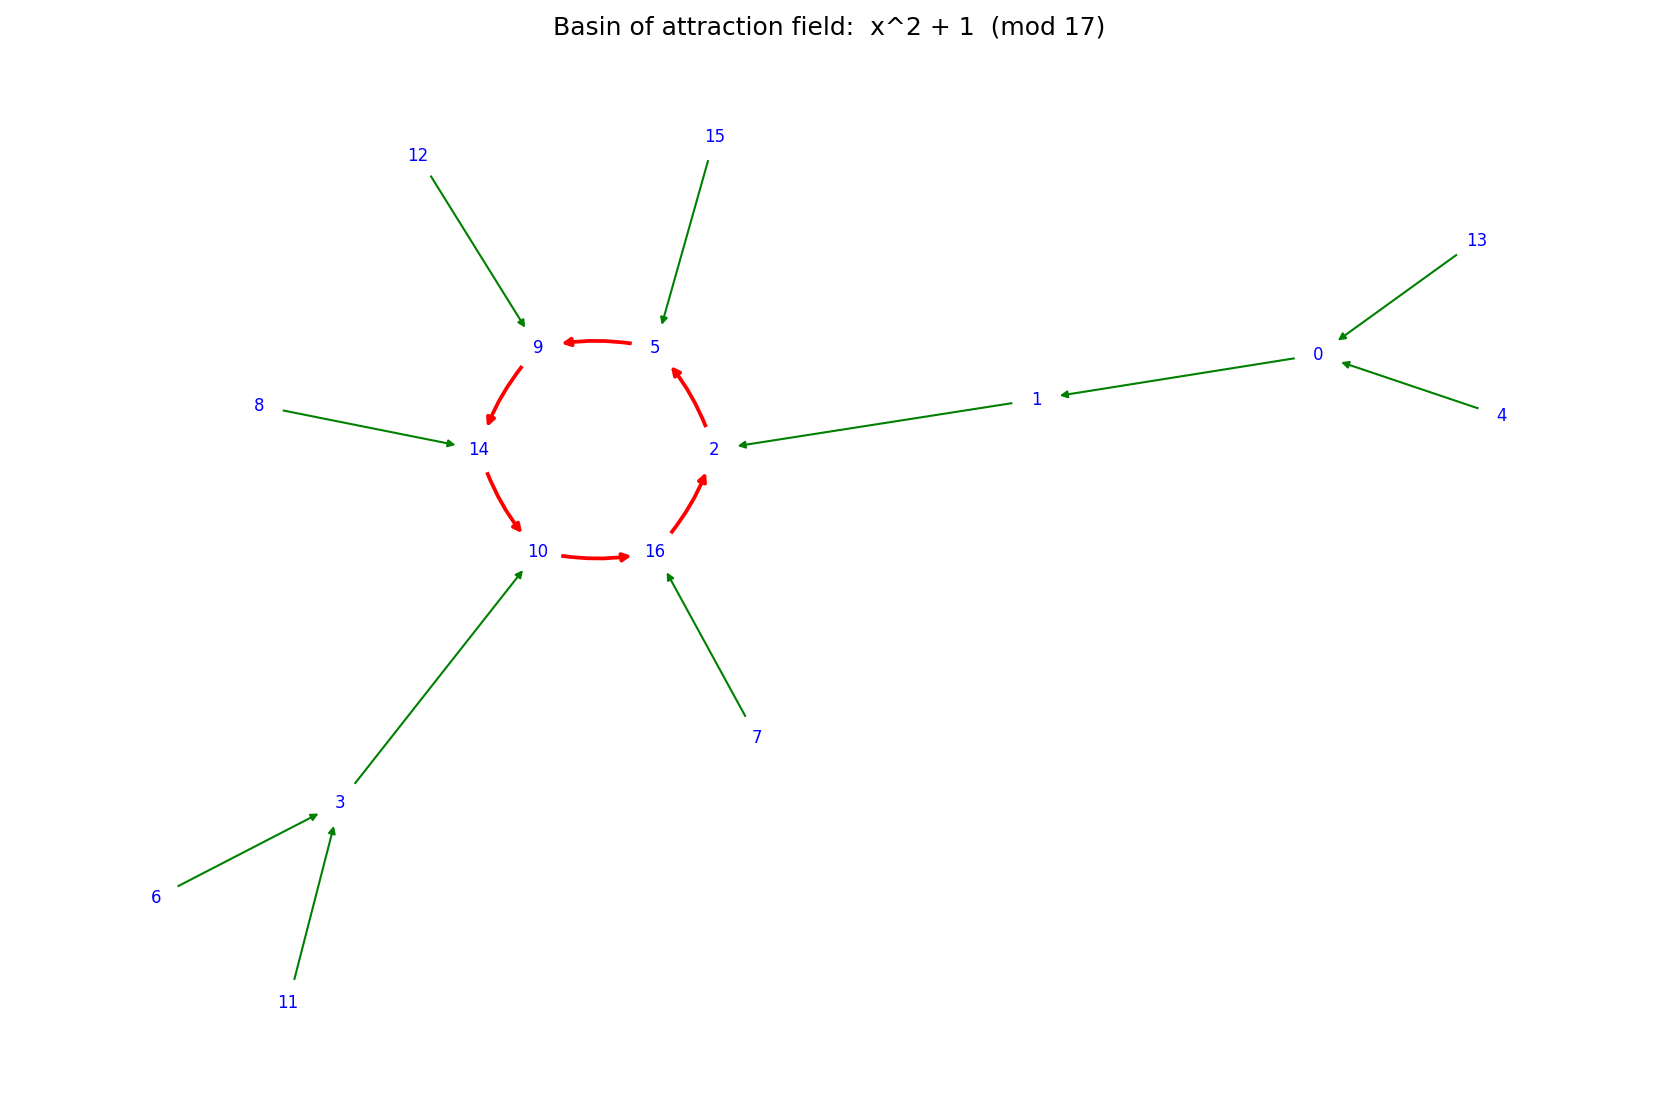
\includegraphics[width=0.8\textwidth]{ch2_basin_mod17}
\caption{Basin of attraction field for $f(x)=x^2+1 \pmod{17}$.  Cycle
edges are red, transient edges green.}
\label{fig:mod17}
\end{figure}

Notice the attractive cycle and the incoming transient branches.  For
this function there is only one attractive cycle; ordinarily there are
several, and the basin-of-attraction field consists of the entire
collection of cycles with their associated transients.  Each node has
exactly one outgoing edge: the system is \emph{deterministic}.  Some
nodes have more than one incoming edge: the system is
\emph{irreversible}, and the entropy of the system tends to decrease as
it evolves.  CA of all dimensions share these qualities, and the
tendency of entropy to decrease in CA is no doubt partly responsible
for the emergent behavior so often evident in such systems.

Notice too that the two predecessors of any node with two predecessors
always sum to $17$.  This follows from the algebraic identity
$x^2 = (-x)^2$ together with the modular-arithmetic fact
$-x \equiv n-x \pmod n$: hence
\[
  x^2 \equiv (n-x)^2, \qquad x^2+1 \equiv (n-x)^2+1,
\]
and so $f(x) \equiv f(n-x) \pmod n$ for $0 \le x \le n-1$.  And indeed
$x + (n-x) = n$.  Here $n=17$, but the same holds for the later
examples using this function; the reader should verify it in
Sections~\ref{sec:mod37} and~\ref{sec:mod221}.

The outermost states in Figure~\ref{fig:mod17}, with values
$4, 6, 7, 8, 11, 12, 13, 15$, have no predecessor states: after one
generation the CA is guaranteed not to occupy any of them.  Such
outlying states are known as \emph{Garden of Eden} states.

Before further examples we digress to define the important concept of
entropy.  Entropy is not separate from information, in precisely the
way the concept of a half-empty glass is not separable from that of a
half-full one; out of this concept grows the entire field of
information theory.

\section{Shannon's Entropy}
\label{sec:entropy}

Entropy for a 0-dimensional CA with $n$ states may be defined via
Shannon's formula
\begin{equation}
  H_t \;=\; -\sum_{k=0}^{n-1} p_t(k)\,\log_2 p_t(k),
\end{equation}
where $p_t(k)$ is the probability that the system has value $k$ after
$t$ time steps from a uniformly random initial value, and where we
agree that $0\log 0 = 0$.  Using base-2 logarithms measures entropy in
\emph{bits}.  $H$ measures the system's basic information potential.

Two extreme cases illuminate the formula.  First, consider a CA in
which every initial state evolves to $0$ (e.g.\ $f(x)=0$).  For $t$
large enough, $p_t(0)=1$ and all other probabilities vanish, so the sum
reduces to $\log_2 1 = 0$: zero entropy.  Entropy connotes randomness
and uncertainty, and here we are \emph{a priori} certain of the
outcome.  Second, consider a CA in which all states remain equally
likely for all time (e.g.\ $f(x)=x+1$).  Then $p_t(k)=1/n$ for all $k$,
and the formula gives
\begin{equation}
  H = -\log_2 \tfrac1n = \log_2 n,
\end{equation}
the maximum entropy possible for a 0-dimensional CA with $n$ states
(Table~\ref{tab:maxent}).  Note that $H$, rounded up, is the number of
binary digits needed to represent $n$.

\begin{table}[htbp]\centering
\begin{tabular}{l|ccccccccc}
\toprule
$n$ & 1 & 2 & 5 & 10 & 15 & 20 & 30 & 50 & 100\\
\midrule
$S=\log_2 n$ & 0 & 1 & 2.32 & 3.32 & 3.91 & 4.32 & 4.91 & 5.64 & 6.64\\
\bottomrule
\end{tabular}
\caption{Maximum entropy $S$ as a function of the number of cell
states $n$.}
\label{tab:maxent}
\end{table}

To compute $p_t(k)$, the software counts the number of initial values
that end up with value $k$ after $t$ iterations; call this
$\mathrm{Num}(k,t)$.  Since there are $n$ equally likely initial
states,
\begin{equation}
  p_t(k) = \frac{\mathrm{Num}(k,t)}{n}.
\end{equation}
$H_0$ is thus always the maximal entropy of the system, and once every
value has settled into a cycle the entropy remains constant at the
system's minimum.\footnote{Strictly, once all transients have died out
the multiset of occupied states is permuted by $f$, so the entropy is
exactly constant from then on.}  In general, the smaller the entropy,
the greater one's \emph{a priori} information about the state of the
system: entropy measures one's uncertainty about a system's state.

\section{Example: $x^2+1 \pmod{37}$}
\label{sec:mod37}

Figure~\ref{fig:mod37} depicts the basin-of-attraction field for
\begin{equation}
  f(x) = x^2 + 1 \pmod{37}.
\end{equation}
There are three separate attractive cycles: two of length~1 (the fixed
points $27$ and $11$) and one of length~2 (the cycle $8, 28$).
Attractive 1-cycles are usually just called \emph{attractors} or
\emph{fixed points}.

\begin{figure}[htbp]\centering
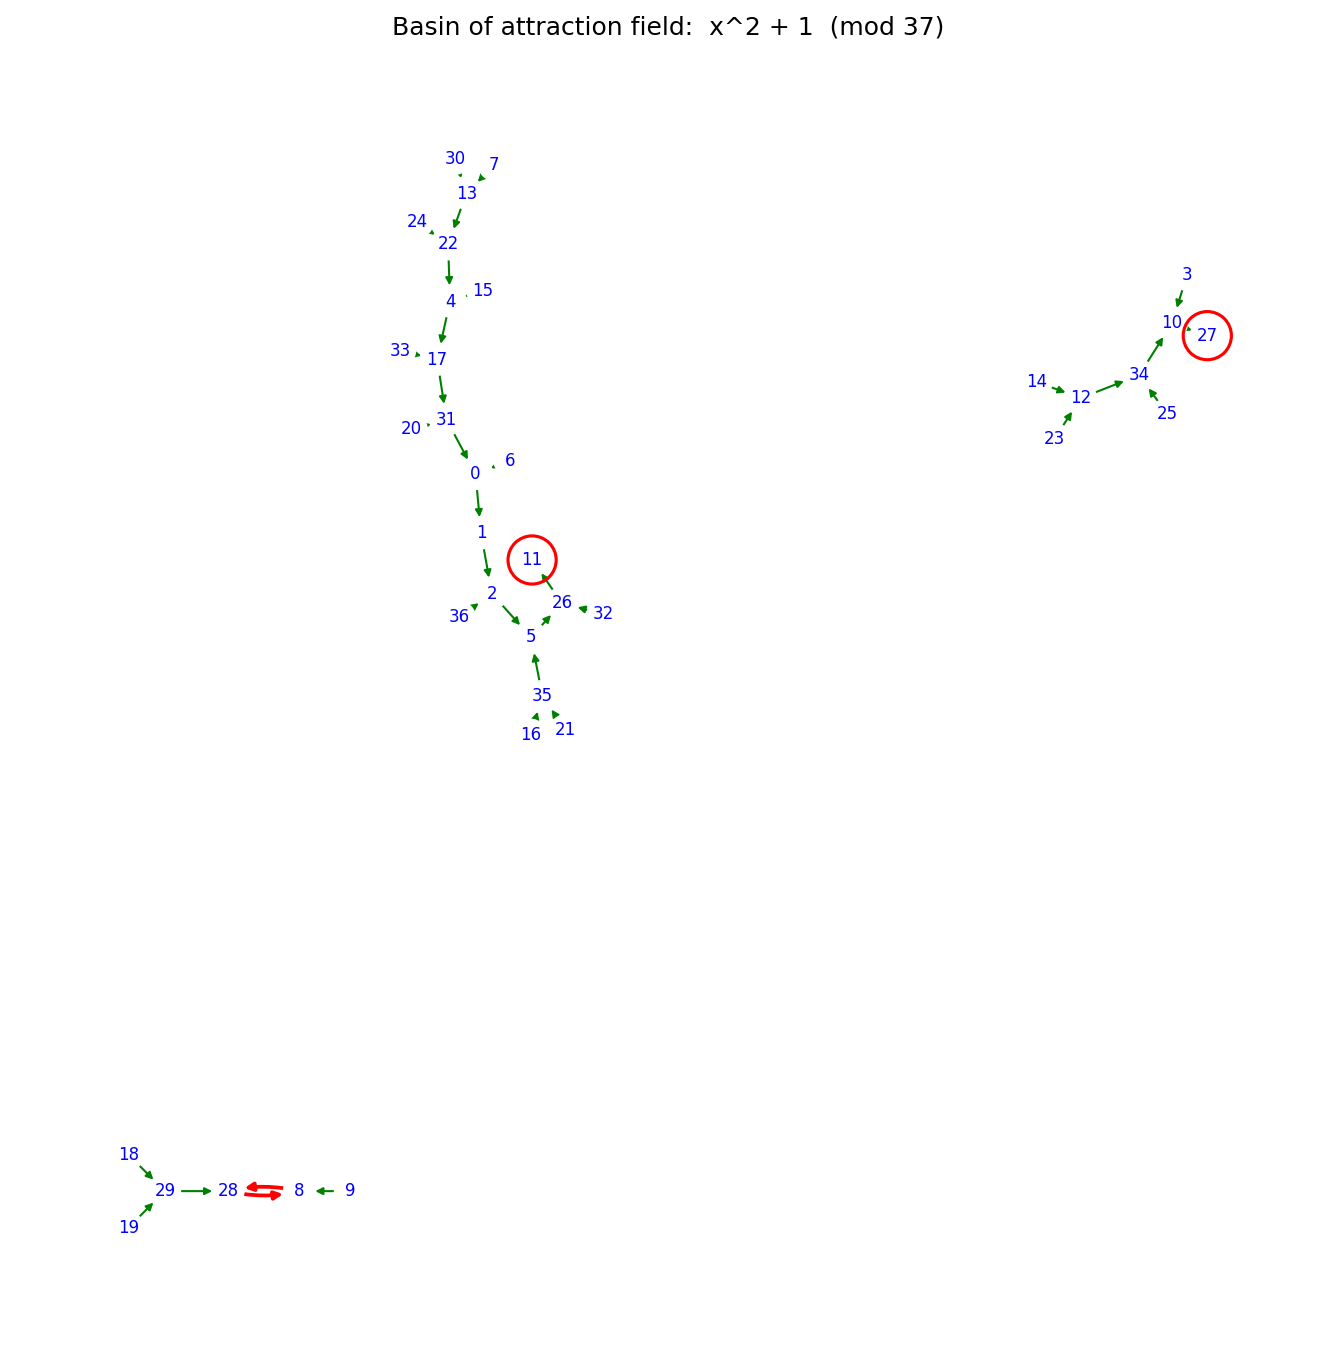
\includegraphics[width=0.9\textwidth]{ch2_basin_mod37}
\caption{Basin of attraction field for $f(x)=x^2+1\pmod{37}$: the
attractor 27 with a basin of 8 states, the 2-cycle $\{8,28\}$ with a
basin of 6 states, and the attractor 11 with a basin of 23 states.}
\label{fig:mod37}
\end{figure}

Since the system eventually evolves to one of four values, the entropy
should be relatively small after six iterations.
Figure~\ref{fig:entropy37} graphs the entropy $H$ as a function of the
number of iterations.

\begin{figure}[htbp]\centering
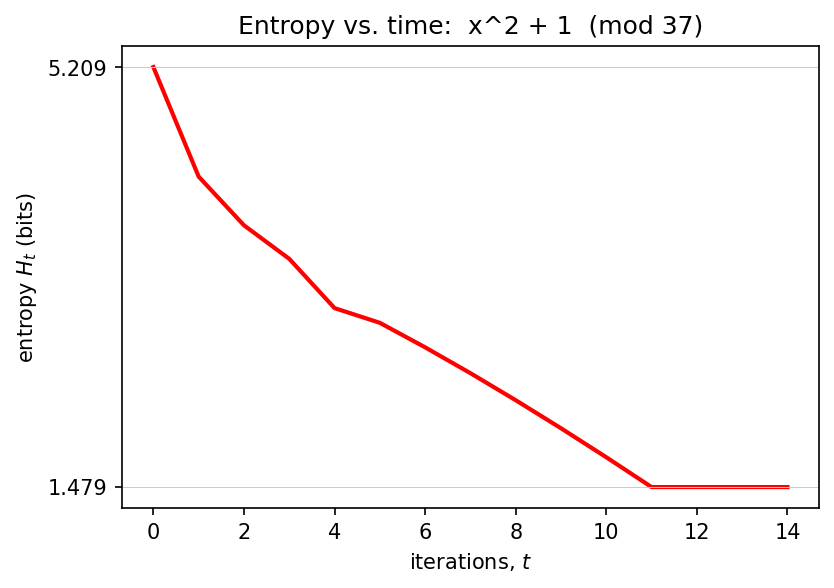
\includegraphics[width=0.65\textwidth]{ch2_entropy_mod37}
\caption{Entropy as a function of time for $f(x)=x^2+1 \pmod{37}$.}
\label{fig:entropy37}
\end{figure}

The system ends up at one of its attractors ($27$ or $11$) or on its
2-cycle $(8,28)$ after 6 time steps, so thereafter it occupies one of
these 4 values.  A uniformly random system with 4 states has entropy
$\log_2 4 = 2$, rather larger than this system's minimum entropy,
$1.478$.  Our smaller final entropy is due mostly to the large number
of transients feeding attractor 11: with 23 states in its basin, the
probability of ending at 11 is $23/37 = 0.621\ldots$, so most of the
time the system ends there.  This additional information means less
uncertainty than in the uniform case, where the probability of ending
at 11 would be only $1/4 = 0.25$; hence the lower entropy.  The greater
one's \emph{a priori} information about a system, the less one's
uncertainty about its states, and the lower its entropy.

\section{Example: $x^2+1 \pmod{221}$}
\label{sec:mod221}

Figure~\ref{fig:mod221} depicts the basin-of-attraction field for
\begin{equation}
  f(x) = x^2 + 1 \pmod{221}.
\end{equation}
In this case there are four separate attractive cycles: two of
length~12 and two of length~6, accounting for the 36 cyclic states.

\begin{figure}[htbp]\centering
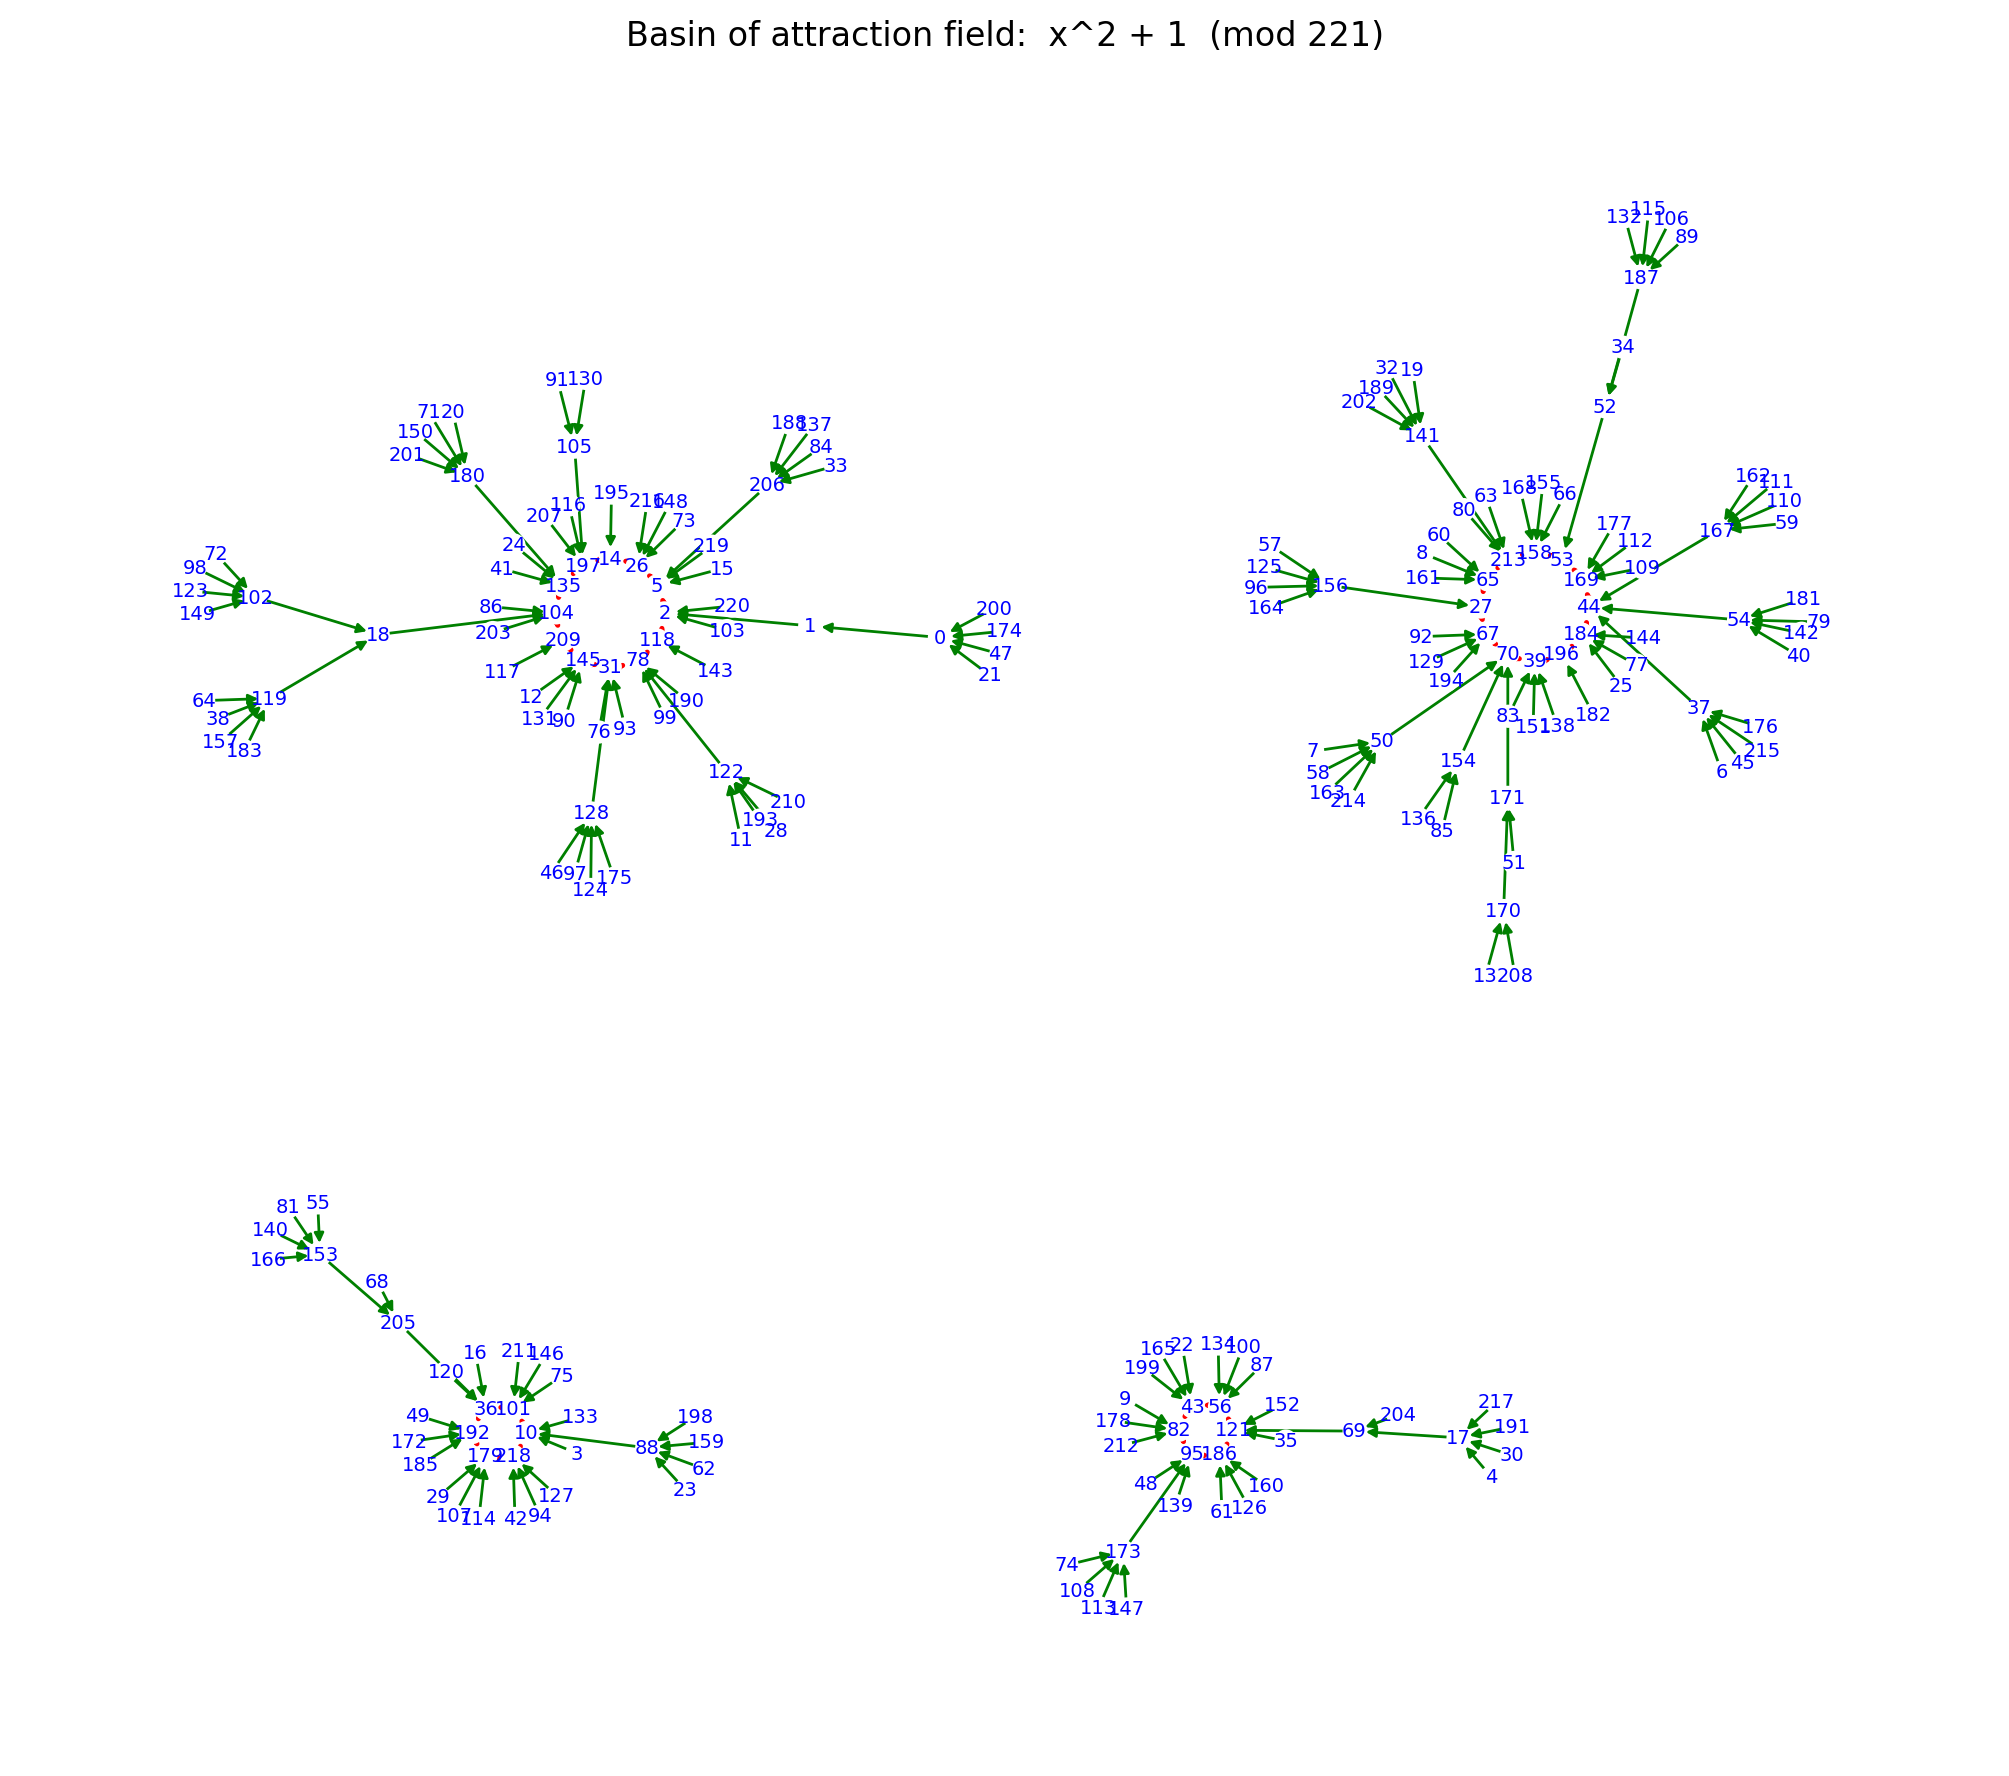
\includegraphics[width=\textwidth]{ch2_basin_mod221}
\caption{Basin of attraction field for $f(x)=x^2+1\pmod{221}$: two
attractive 12-cycles and two attractive 6-cycles, with their
transients.  Note the topological repetition between basins of equal
cycle length.}
\label{fig:mod221}
\end{figure}

The topological repetition observed among basins of attraction is very
common for large moduli, and the redundancy becomes even more
pronounced for CA on higher-dimensional lattices.\footnote{For this
example the repetition has a tidy explanation: $221 = 13\cdot17$, and
by the Chinese Remainder Theorem the system is the direct product of
$x^2+1$ mod 13 and mod 17, whose cycle structures combine to produce
the paired 6- and 12-cycles.}
Figure~\ref{fig:entropy221} shows the entropy graph for this system.
The outcome of many iterations is far less certain than for the system
of Section~\ref{sec:mod37}, so the minimum entropy is higher
($H_{\min}=4.983$ versus $1.478$).

\begin{figure}[htbp]\centering
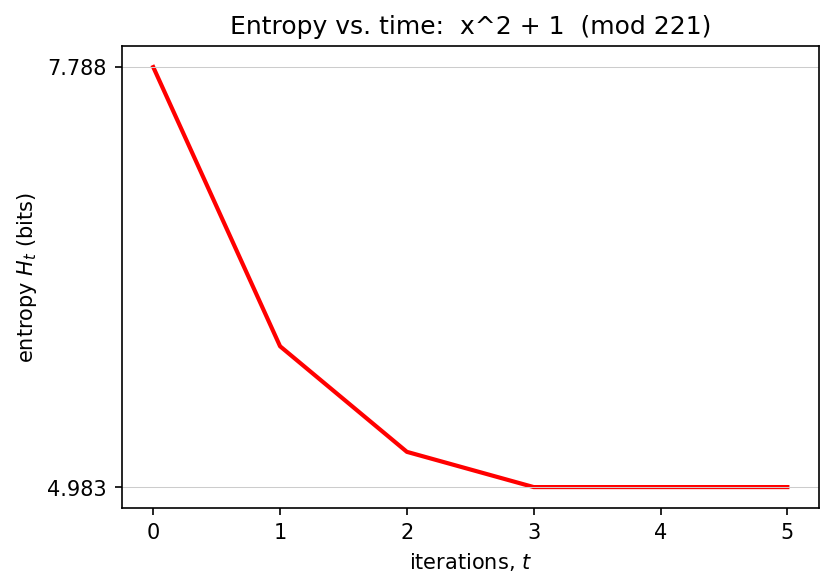
\includegraphics[width=0.65\textwidth]{ch2_entropy_mod221}
\caption{Entropy as a function of time for $f(x)=x^2+1 \pmod{221}$.}
\label{fig:entropy221}
\end{figure}

The system reaches one of its 4 cycles after 3 time steps and is
thereafter confined to the 36 cyclic values.  A uniformly random system
with 36 states has entropy $\log_2 36 = 5.170$, very close to this
system's minimum entropy.  Our slightly smaller final entropy is due to
the greater number of transients associated with the 12-cycles, which
makes ending in a 12-cycle more probable than ending in a 6-cycle; this
extra information lowers the entropy below that of a uniformly random
system.

\section{Example: $x^3 + 2x^2 + 3x + 2 \pmod{28}$}
\label{sec:cubic}

Figure~\ref{fig:cubic} shows the basin-of-attraction field for
\begin{equation}
  f(x) = x^3 + 2x^2 + 3x + 2 \pmod{28},
\end{equation}
whose basin-of-attraction field comprises two basins: an attractive
6-cycle and an attractive 2-cycle, each with associated transients.
Figure~\ref{fig:entropycubic} shows the entropy graph.

\begin{figure}[htbp]\centering
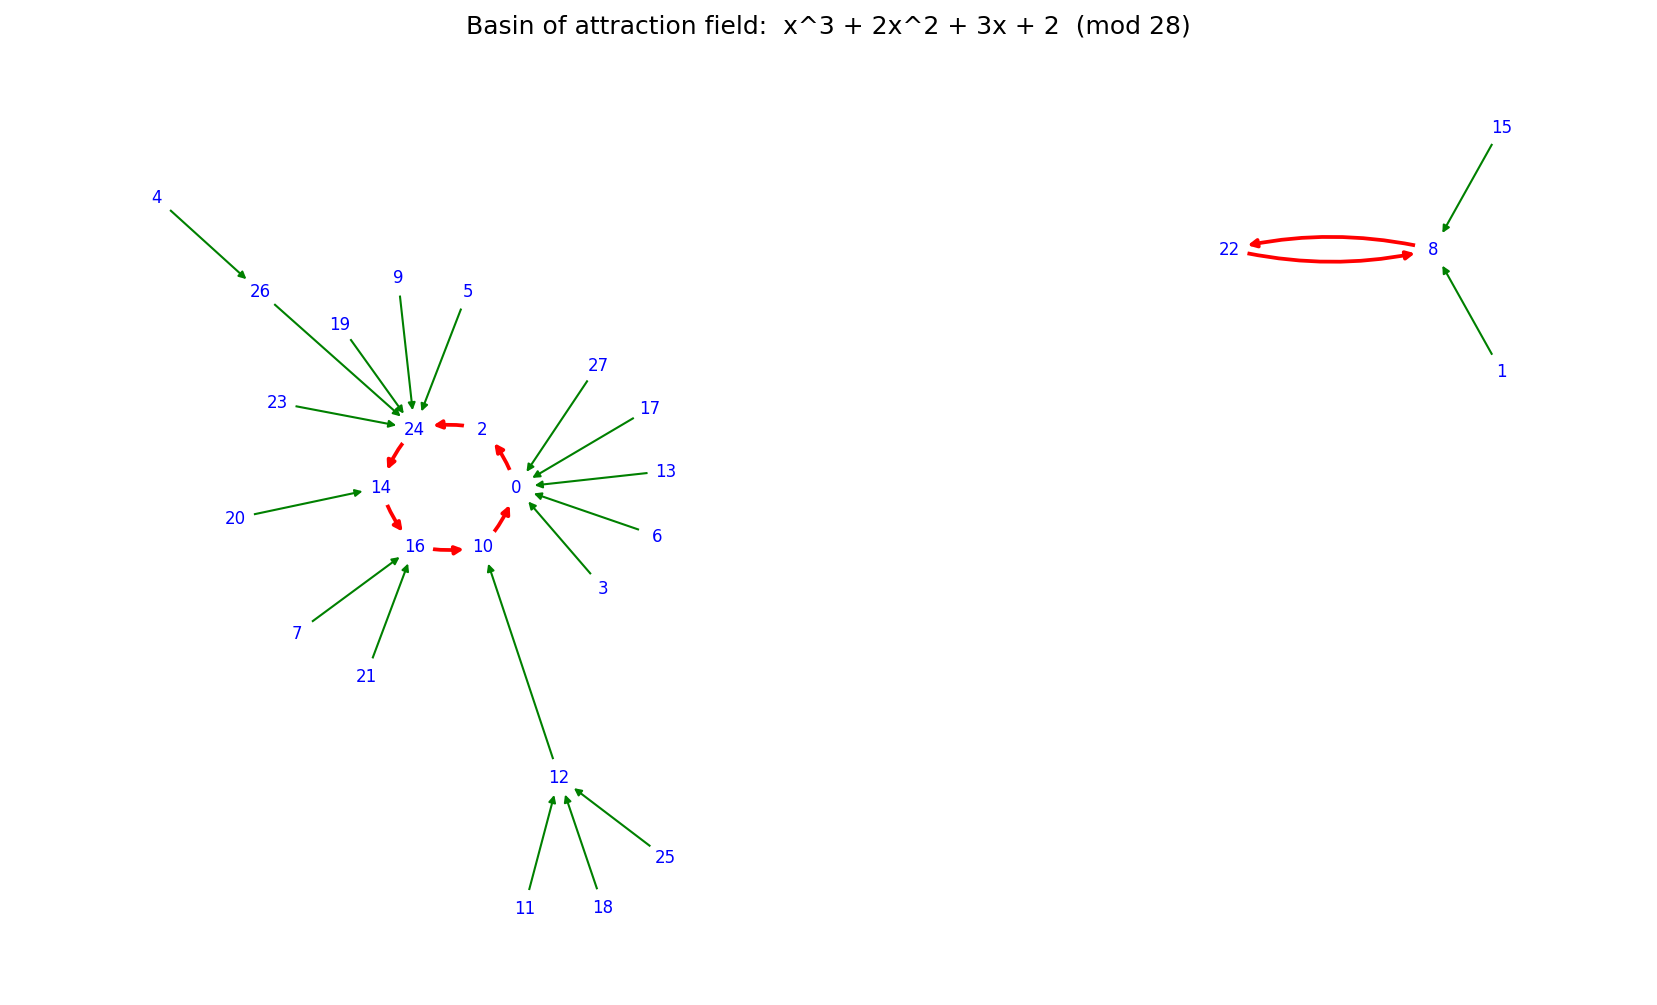
\includegraphics[width=0.8\textwidth]{ch2_basin_cubic_mod28}
\caption{Basin of attraction field for
$f(x)=x^3+2x^2+3x+2 \pmod{28}$: an attractive 6-cycle and an
attractive 2-cycle.}
\label{fig:cubic}
\end{figure}

\begin{figure}[htbp]\centering
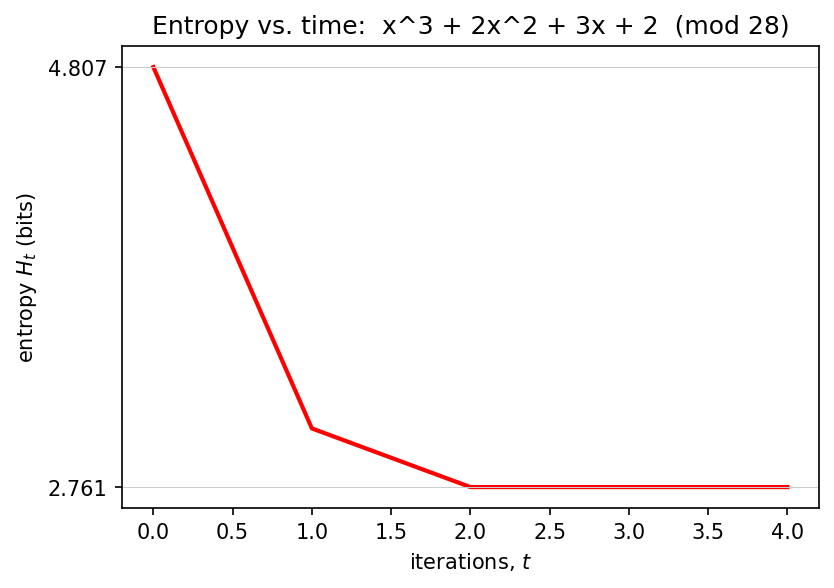
\includegraphics[width=0.65\textwidth]{ch2_entropy_cubic_mod28}
\caption{Entropy as a function of time for
$f(x)=x^3+2x^2+3x+2 \pmod{28}$.}
\label{fig:entropycubic}
\end{figure}

\section{Ulam's Function}
\label{sec:ulam}

In the late 1940s Stanis\l{}aw Ulam introduced the $3N+1$ problem to
the Los Alamos scientific community (though he didn't invent it), which
was beginning to play with the very first digital computers.  The
problem involves a simple recursively defined arithmetic function that
to this day holds unfathomed mysteries:
\begin{equation}
  f(n) =
  \begin{cases}
    n/2, & \text{if } n \text{ even};\\
    3n+1, & \text{if } n \text{ odd}.
  \end{cases}
\end{equation}
The observation Ulam circulated is that no matter what positive integer
one starts with, iterating $f$ appears always to arrive at the
attractive cycle $4\to2\to1$.  Nobody knows whether \emph{all} positive
integers belong to this cycle's basin of attraction.

\expand{The conjecture (also attached to the names Collatz, Kakutani,
Syracuse, and others) remains open.  The first edition noted
verification for all $n < 10^{12}$; as of the mid-2020s it has been
verified for all $n < 2^{71} \approx 2.36\times10^{21}$ (Barina 2020
and subsequent distributed computation), and Terence Tao proved in 2019
that ``almost all'' orbits attain almost bounded values --- yet a full
proof remains out of reach, vindicating Erd\H{o}s's judgment that
``mathematics is not yet ripe for such problems.''}

If zero is allowed as an argument, it becomes another attractor.  The
module \texttt{cadyn.fds} has this function built in, modulo arbitrary
values, and when computed with modular arithmetic zero has its own
basin of attraction.  Figure~\ref{fig:ulam} shows the computation
modulo 20 and modulo 40, and Figure~\ref{fig:ulam47} the computation
modulo 47.  Notice the surprising occurrence
of yet another attractor, $23$, in the modulus-47 case.

\begin{figure}[htbp]\centering
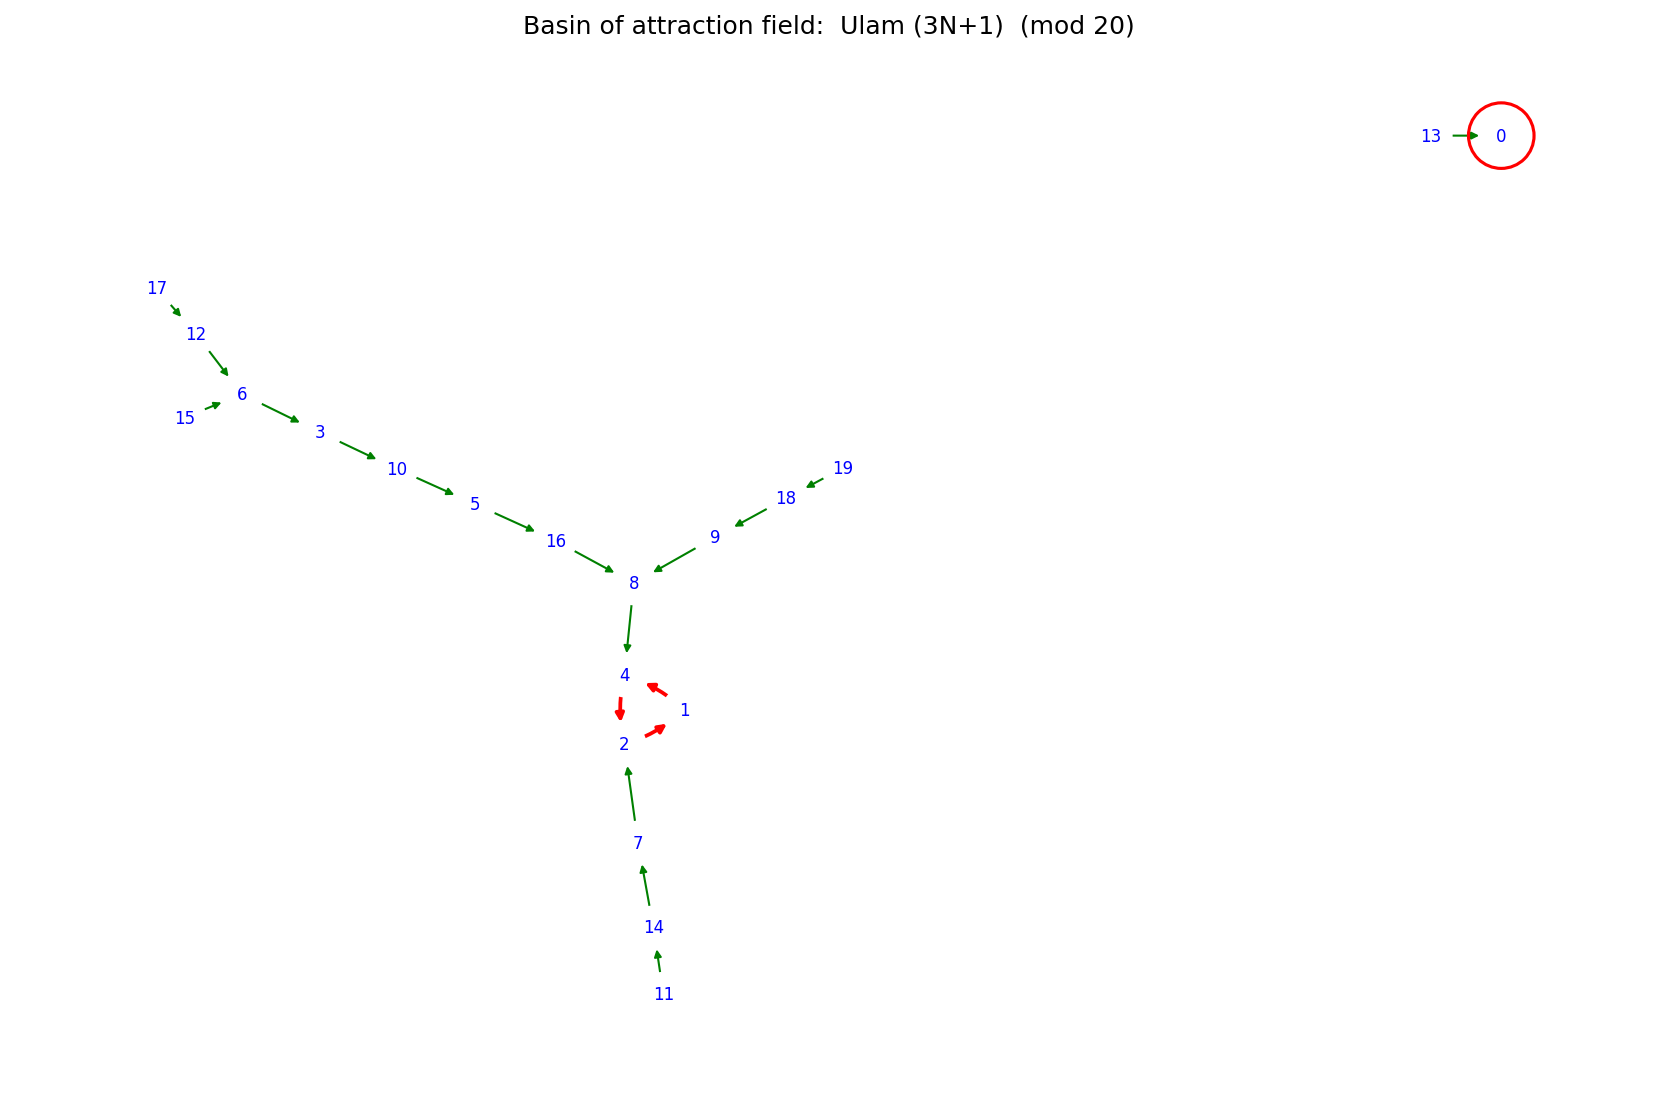
\includegraphics[width=0.88\textwidth]{ch2_basin_ulam_mod20}\\[1.5ex]
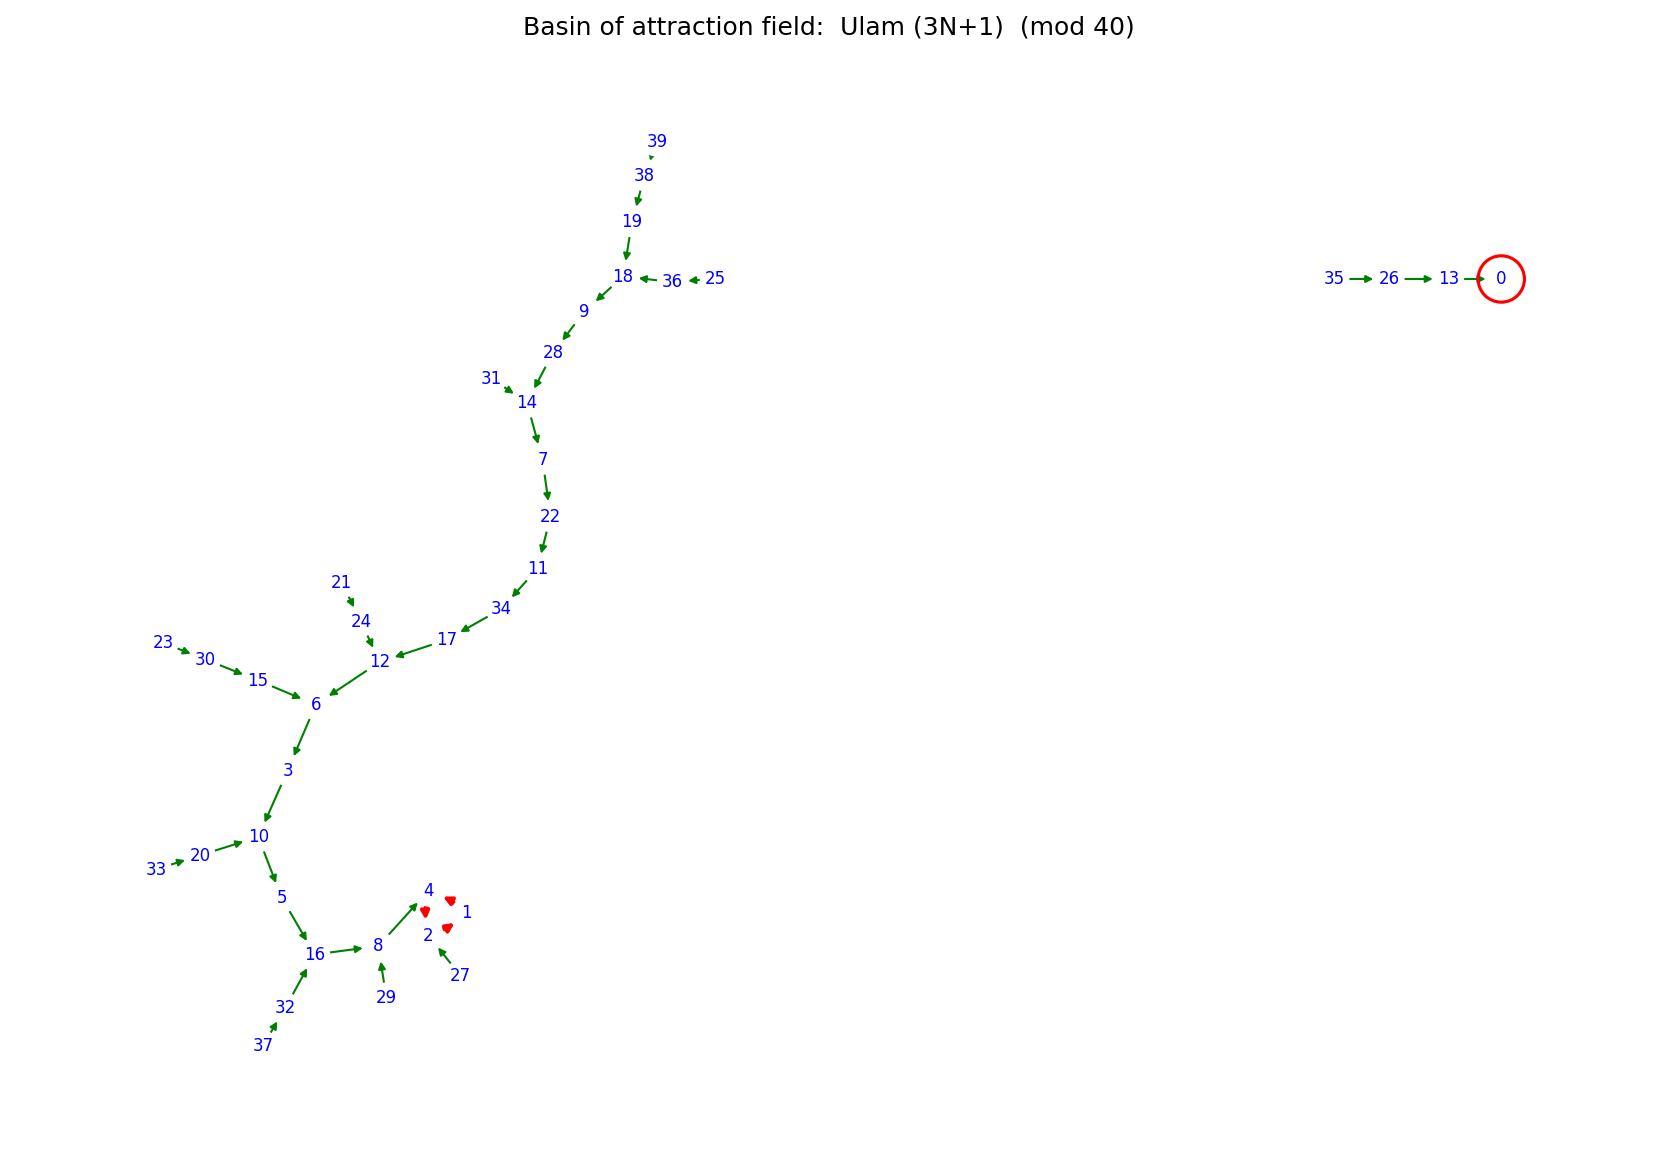
\includegraphics[width=0.88\textwidth]{ch2_basin_ulam_mod40}
\caption{Ulam's function modulo 20 (top) and 40 (bottom).}
\label{fig:ulam}
\end{figure}

\begin{figure}[htbp]\centering
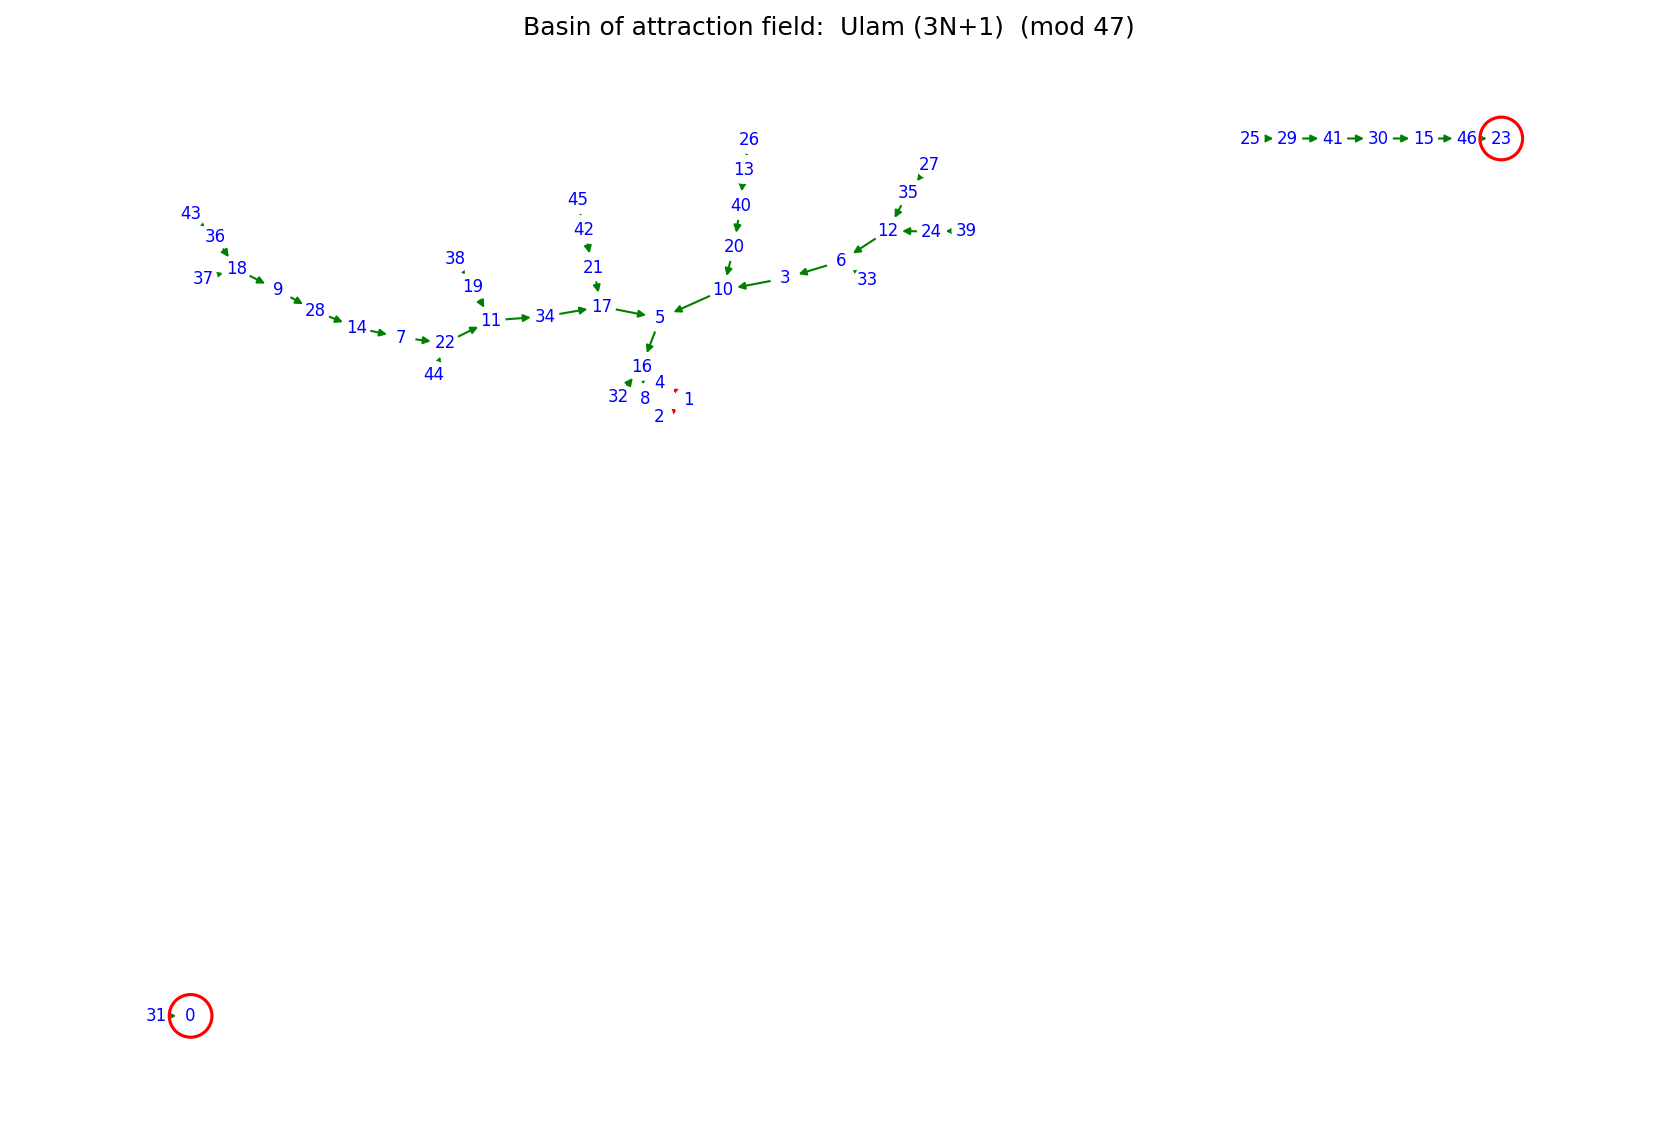
\includegraphics[width=0.95\textwidth]{ch2_basin_ulam_mod47}
\caption{Ulam's function modulo 47, with the surprise attractor
at 23.}
\label{fig:ulam47}
\end{figure}

\begin{figure}[htbp]\centering
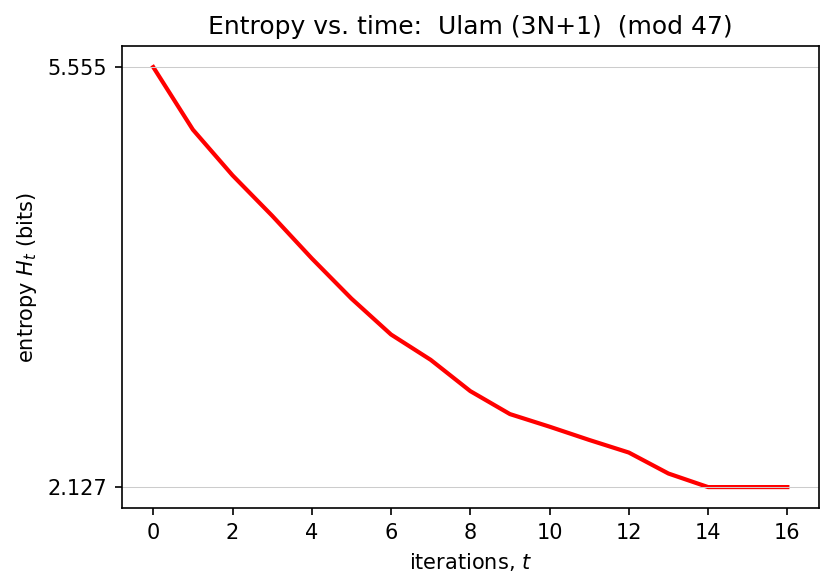
\includegraphics[width=0.62\textwidth]{ch2_entropy_ulam_mod47}
\caption{Entropy history for Ulam's function modulo 47.}
\label{fig:ulam-entropy}
\end{figure}

\chapter{1-Dimensional Cellular Automata}

\section{Preliminaries}

As a paradigm for parallel processing, 0-dimensional CA aren't really
CA at all --- parallel processing is meaningless with only one
processor.  We need at least one dimension to have a \emph{real} CA;
this is where most treatises on CA begin, so now we're off to confront
the real beast.

A one-dimensional lattice is an array of cells distributed along a
line, each taking a value from a finite set at each tick of the clock.
We denote the state of the CA at time $t$ by
\[
  C^{(t)} = \cdots\,
  C^{(t)}_{-2}\; C^{(t)}_{-1}\; C^{(t)}_{0}\; C^{(t)}_{1}\;
  C^{(t)}_{2}\,\cdots.
\]
We consider only CA with \emph{periodic boundary conditions}, a
technique for making infinite arrays effectively finite.  Fixing a
specific number of cells $n$, the infinite array becomes the finite
array
\[
  C^{(t)} = C^{(t)}_{0}\; C^{(t)}_{1}\; C^{(t)}_{2}\;\cdots\;
  C^{(t)}_{n-2}\; C^{(t)}_{n-1}.
\]
Mentally connect the two ends of this queue to form a circle, so that
$C^{(t)}_0$ and $C^{(t)}_{n-1}$ are adjacent.  Equivalently, one may
define initial conditions on cells $0$ through $n-1$ and repeat this
pattern endlessly to the right and left, so that any two cells whose
indices are congruent modulo $n$ carry the same value:
\begin{equation}
  b \equiv d \pmod n \;\Longrightarrow\; C^{(t)}_b = C^{(t)}_d.
\end{equation}
In short, all arithmetic on cell indices is performed modulo $n$.

Although CA neighborhoods may in general be arbitrary, for the CA we
examine the same relative neighborhood is defined for every cell (such
CA are called \emph{homogeneous}).  We let $k$ denote the number of
states per cell, identify the states with $0,1,\dots,k-1$, and perform
computations on cell values modulo $k$.

Before the examples we discuss a useful representation of a class of CA
transition rules, borrowed from 1-dimensional digital signal
processing: \emph{convolution kernels}.

\section{Transition Rules as Convolution Kernels}

In digital signal processing one of the most basic tools, borrowed from
differential equations, is convolution.  Students of differential
equations first meet a continuous version of this concept in the
Laplace transform.  For discrete signals the convolution operation is
equivalent to applying a CA to the signal: take the signal as the
initial condition, and let the convolution kernel define the transition
rule.  The computation a computer performs for one convolution is
identical to one generation of the corresponding CA.  The difference is
one of intent: a convolution is applied once (or a few times) to
produce a filtered output signal, whereas a CA iterates its recursion
for many generations, even endlessly.

Not all CA can be represented by convolution kernels; those that can
are called \emph{additive}.  Of this chapter's examples, those of
Sections 3.2--3.5 are additive, while the sum-of-squares rule
(Section~\ref{sec:sumsq}) and the 1-dimensional Life
(Section~\ref{sec:life1d}) are not.

To see how a 1-dimensional kernel is applied, we convolve the kernel
$[1\;2\;1]$ with the signal $0\;0\;3\;4\;5\;0\;0$.  Position the kernel
over the beginning of the signal and form the inner product:
$1\cdot0 + 2\cdot0 + 1\cdot3 = 3$, the first value of the output
(``filtered'') signal.  Shift the kernel one position right and
repeat: $1\cdot0+2\cdot3+1\cdot4 = 10$; then
$1\cdot3+2\cdot4+1\cdot5=16$; then $1\cdot4+2\cdot5+1\cdot0=14$; and
finally $1\cdot5+2\cdot0+1\cdot0=5$.  The output signal is
$3\;10\;16\;14\;5$ --- two entries shorter than the input.  Often one
wants output of the same length; one may \emph{pad} the input with
zeros at each end, or use \emph{wrap-around}, where the value to the
left of the leftmost entry is taken to be the rightmost entry and
conversely --- joining the ends of a string into a loop, i.e.\ imposing
periodic boundary conditions.

In mathematical notation, the convolution of a signal
$x_0\, x_1 \dots x_{n-1}$ with a kernel of length $2m+1$,
\[
  [\,k_{-m},\ \dots,\ k_{-1},\ k_0,\ k_1,\ \dots,\ k_m\,],
\]
under periodic boundary conditions, is
\begin{equation}
  y_h \;=\; \sum_{l=-m}^{m} k_l\, x_{(h+l) \bmod n},
  \label{eq:conv1d}
\end{equation}
where $y_0y_1\dots y_{n-1}$ is the output signal; we take the sum
modulo $k$.  Here we follow signal-processing terminology in calling
the arrays signals; the same algorithm applies to arrays considered as
CA states, the input state being one generation and the output the
next.

With 1-dimensional CA we can see the whole evolution at a glance by
displaying successive generations as successive rows (or columns) of
pixels.  For higher-dimensional CA we must resort to other techniques.

\section{Example: $k=5$, $n=21$, kernel $[1\;1\;1]$}
\label{sec:k5n21}

Here $k=5$ and the number of cells is $n=21$, so each generation is a
21-component vector $C_0C_1\cdots C_{20}$ with entries from
$\{0,1,2,3,4\}$ --- each state a 21-digit base-5 number.  The cell ``to
the left'' of $C_0$ is $C_{20}$, and the cell ``to the right'' of
$C_{20}$ is $C_0$.  The neighborhood of a cell is the cell itself with
its left and right neighbors, and the transition rule is the sum of the
neighborhood, modulo 5:
\begin{equation}
  C^{(t+1)}_j = T(C^{(t)}_{j-1}, C^{(t)}_j, C^{(t)}_{j+1})
  = C^{(t)}_{j-1} + C^{(t)}_j + C^{(t)}_{j+1} \pmod 5,
\end{equation}
with subscript arithmetic modulo 21.  We start from the simplest
initial state, all zeros except a single one:

\begin{center}\ttfamily\small
\begin{tabular}{ll}
Gen 0: & 0 0 0 0 0 0 0 0 0 0 1 0 0 0 0 0 0 0 0 0 0\\
Gen 1: & 0 0 0 0 0 0 0 0 0 1 1 1 0 0 0 0 0 0 0 0 0\\
Gen 2: & 0 0 0 0 0 0 0 0 1 2 3 2 1 0 0 0 0 0 0 0 0\\
Gen 3: & 0 0 0 0 0 0 0 1 3 1 2 1 3 1 0 0 0 0 0 0 0\\
Gen 4: & 0 0 0 0 0 0 1 4 0 1 4 1 0 4 1 0 0 0 0 0 0\\
Gen 5: & 0 0 0 0 0 1 0 0 0 0 1 0 0 0 0 1 0 0 0 0 0\\
Gen 6: & 0 0 0 0 1 1 1 0 0 1 1 1 0 0 1 1 1 0 0 0 0\\
Gen 7: & 0 0 0 1 2 3 2 1 1 2 3 2 1 1 2 3 2 1 0 0 0\\
Gen 8: & 0 0 1 3 1 2 1 4 4 1 2 1 4 4 1 2 1 3 1 0 0\\
Gen 9: & 0 1 4 0 1 4 2 4 4 2 4 2 4 4 2 4 1 0 4 1 0\\
\end{tabular}
\end{center}

A run of 136 generations produced Figure~\ref{fig:k5n21}, in which the
first generation is the leftmost column.  Black${}=0$, blue${}=1$,
green${}=2$, orange${}=3$, red${}=4$.

\begin{figure}[htbp]\centering
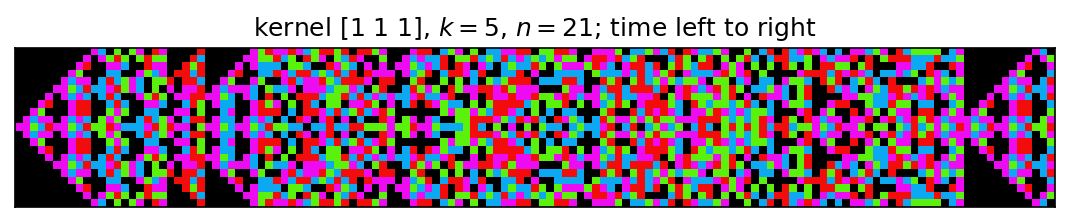
\includegraphics[width=\textwidth]{ch3_k5_n21_kernel111}
\caption{136 generations, one generation per column; time increases
left to right.}
\label{fig:k5n21}
\end{figure}

The transition rule is exactly convolution with the kernel $[1\;1\;1]$:
the inner product of the kernel with consecutive cells yields the new
value of the center cell.  With 5 states per cell and 21 cells the
number of possible CA states is
\[
  5^{21} = 476{,}837{,}158{,}203{,}125,
\]
which makes it difficult to display the basin-of-attraction field!
Computer programs have computed basin-of-attraction fields for a great
many 1-dimensional CA with two states, and an atlas of these has been
published (Wuensche and Lesser).  These fields are highly reminiscent
of those of 0-dimensional CA, though more complex.  Most CA exhibit
decreasing Shannon entropy as time proceeds, as in the 0-dimensional
case; determinism precludes an entropy increase, since each node of the
basin-of-attraction field has exactly one out-edge.

The periodicity observed in Figure~\ref{fig:k5n21} is a cycle of length
124 beginning with the state $\dots0\,0\,1\,1\,1\,0\,0\dots$ of
generation~1.  Our initial state $\dots0\,0\,1\,0\,0\dots$ is a
transient (of length one) in the basin of attraction of this attractive
cycle, so the pattern of generation $t$ first recurs at generation
$t+124$ (for $t \ge 1$).  Such eventual periodicity is inevitable for
every CA with finitely many cells.

\section{Examples: $n=512$, kernel $[1\;0\;1]$, various $k$}
\label{sec:kernel101}

For $k=2$ and $n=512$, each state is a 512-component binary vector ---
a 512-digit binary number.  The neighborhood of a cell is the pair of
adjacent cells (the cell itself \emph{not} included), and the rule is
their sum mod 2, i.e.\ convolution with $[1\;0\;1]$:
\begin{equation}
  C^{(t+1)}_j = C^{(t)}_{j-1} + C^{(t)}_{j+1} \pmod k .
  \label{eq:rule101}
\end{equation}

Starting from a single seed, 256 generations produce the pattern of
Figure~\ref{fig:sierp2} --- successive approximations to the fractal
known as \emph{Sierpi\'nski's gasket} (see
Appendix~\ref{app:sierpinski}).  The number of possible states of this
CA is $2^{512} \approx 10^{154}$, considerably greater than the number
of fundamental particles in the universe; we forgo printing the
complete basin-of-attraction field.

\begin{figure}[htbp]\centering
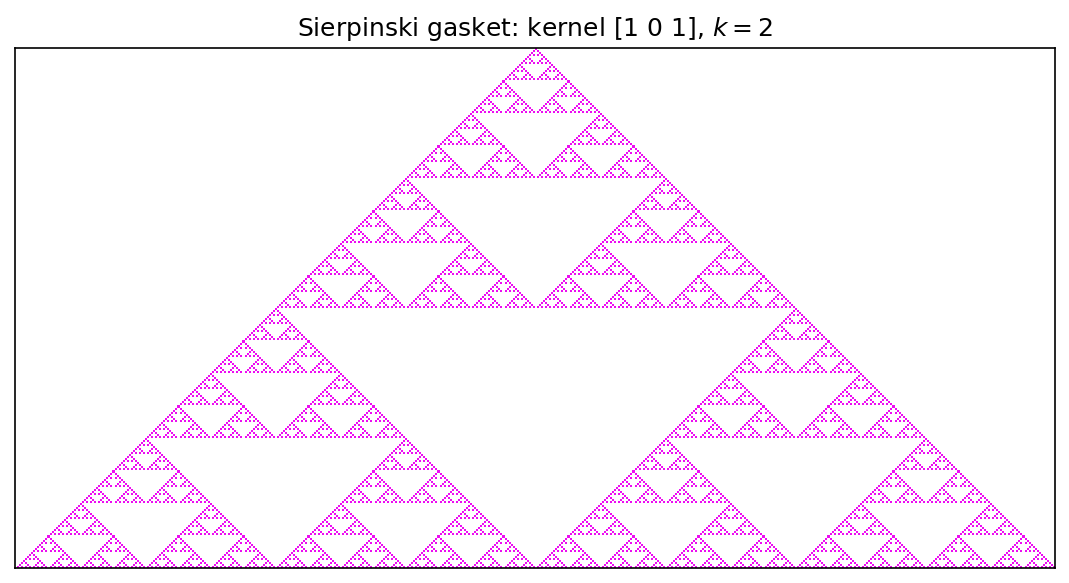
\includegraphics[width=0.8\textwidth]{ch3_sierpinski_k2}
\caption{Sierpi\'nski gasket generated by the CA with kernel
$[1\;0\;1]$, $k=2$.}
\label{fig:sierp2}
\end{figure}

Interesting patterns are obtained from the same rule
\eqref{eq:rule101} with more states, taking larger moduli.
Figure~\ref{fig:sierpk} shows the patterns for
$k = 3, 4, 5, 15, 17, 29, 30$.  White represents cell value 0; colors
represent the other $k-1$ states.  Notice that for prime moduli the
patterns are simpler and more regular, and that the complexity
increases with the number of factors of the modulus.

\begin{figure}[p]\centering
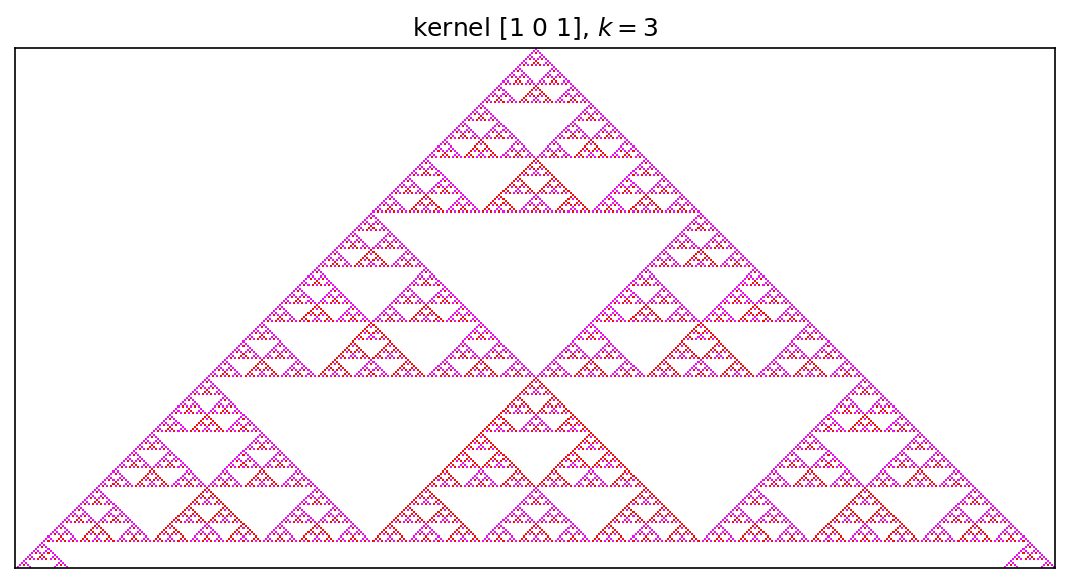
\includegraphics[width=0.42\textwidth]{ch3_kernel101_k3}\;
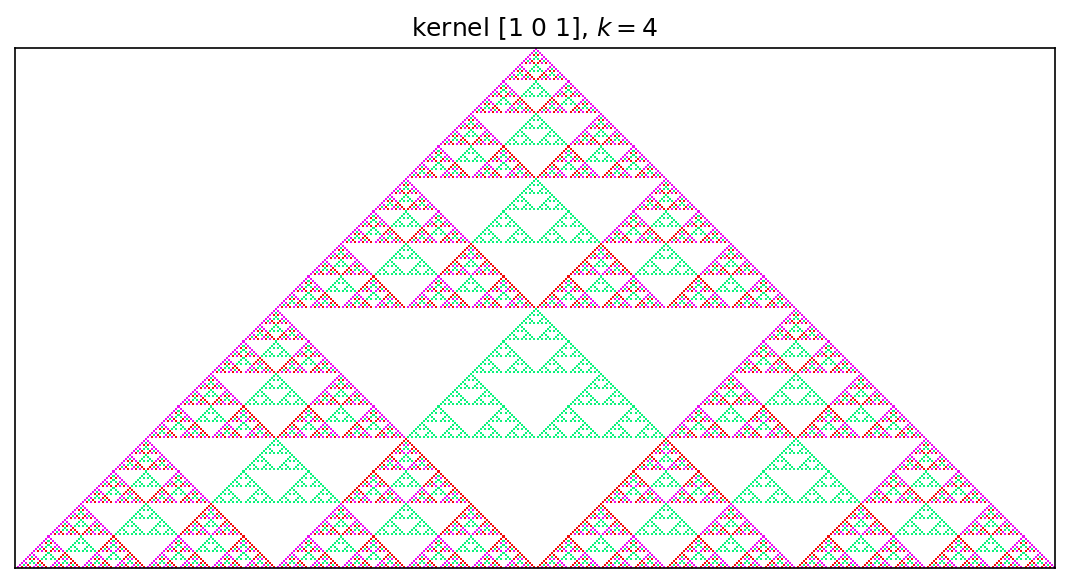
\includegraphics[width=0.42\textwidth]{ch3_kernel101_k4}\\[0.5ex]
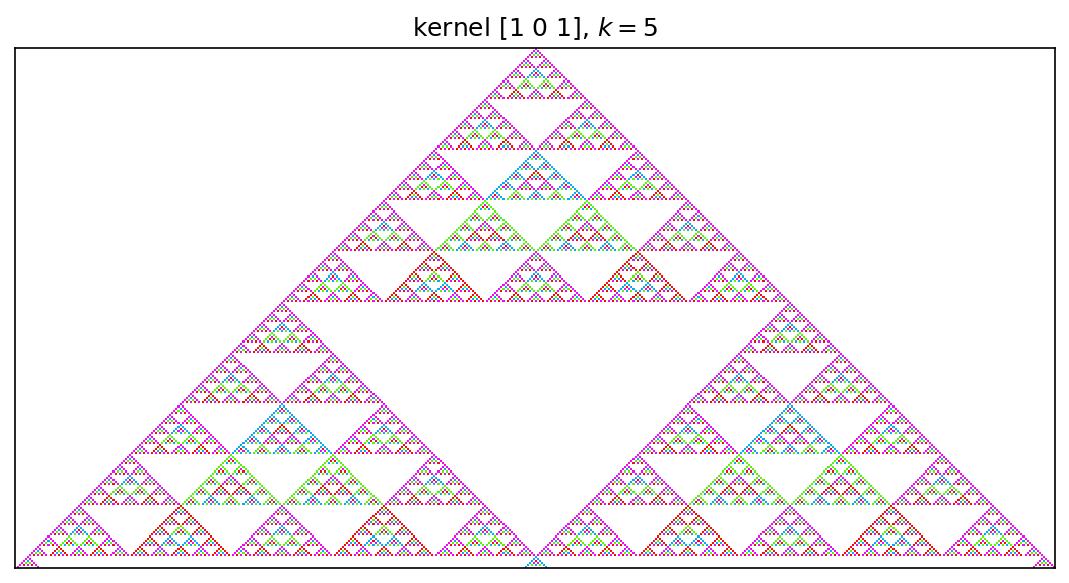
\includegraphics[width=0.42\textwidth]{ch3_kernel101_k5}\;
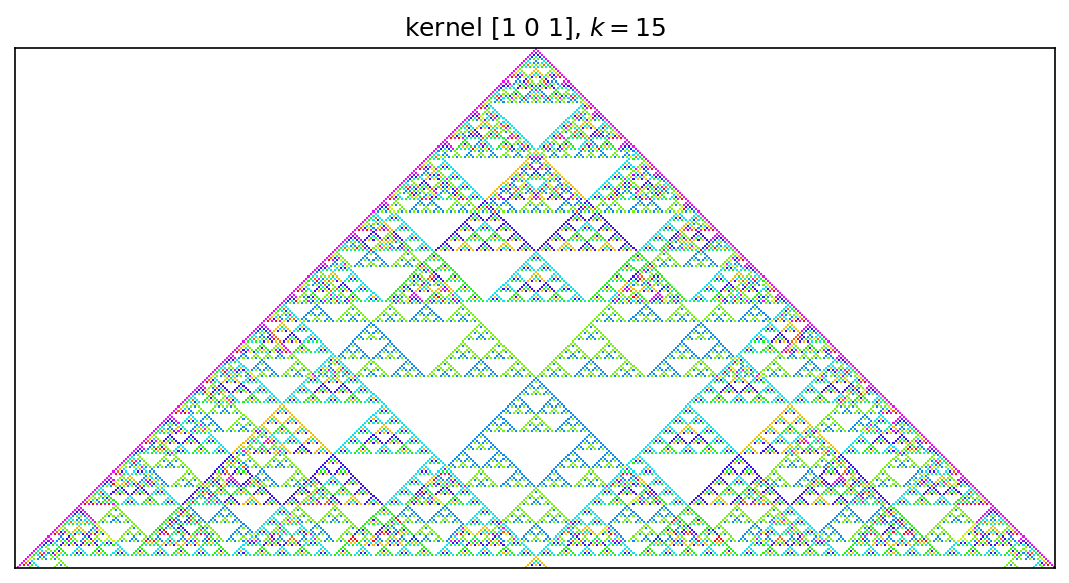
\includegraphics[width=0.42\textwidth]{ch3_kernel101_k15}\\[0.5ex]
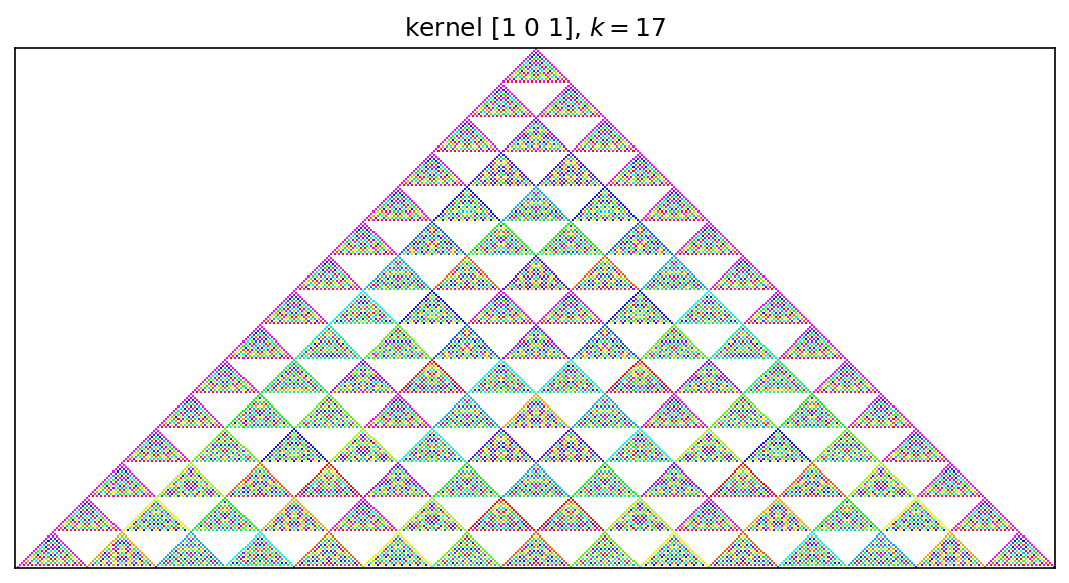
\includegraphics[width=0.42\textwidth]{ch3_kernel101_k17}\;
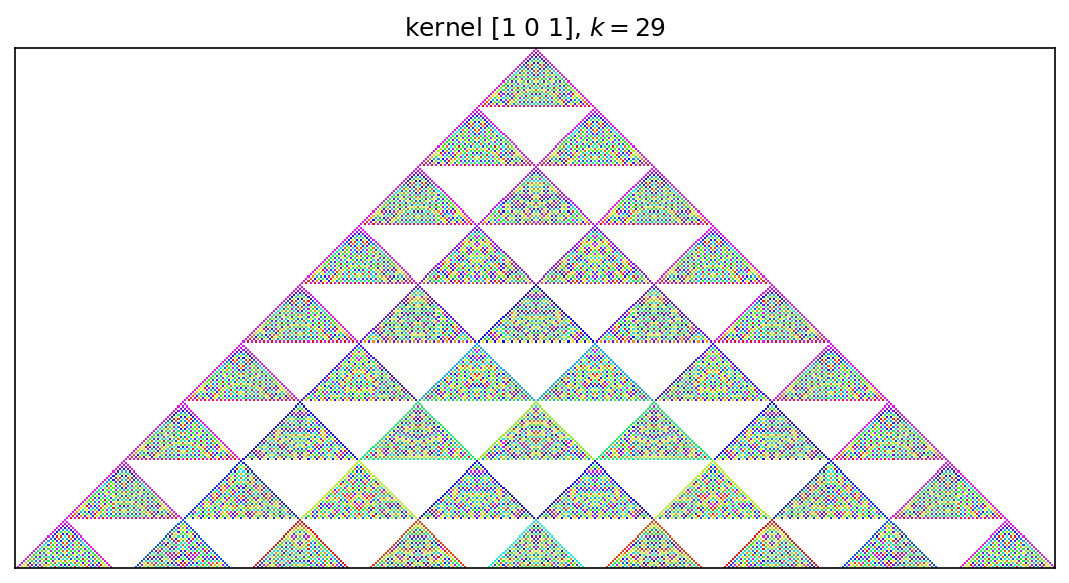
\includegraphics[width=0.42\textwidth]{ch3_kernel101_k29}\\[0.5ex]
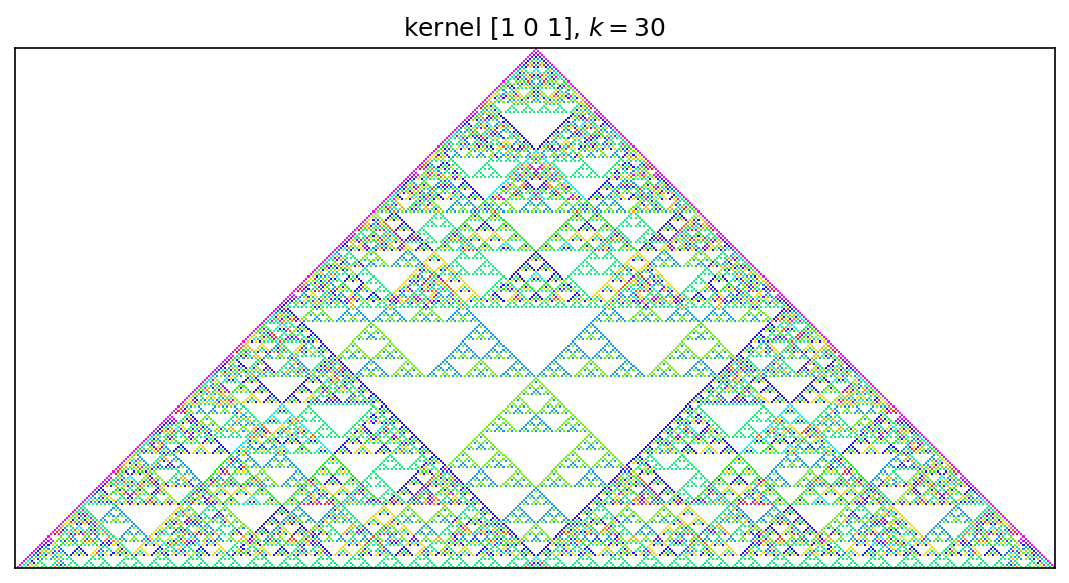
\includegraphics[width=0.42\textwidth]{ch3_kernel101_k30}
\caption{Kernel $[1\;0\;1]$, $n=512$, for (left to right, top to
bottom) $k = 3, 4, 5, 15, 17, 29, 30$.}
\label{fig:sierpk}
\end{figure}

\section{Polynomial Representation of Additive CA}
\label{sec:poly1d}

Additive CA --- those whose transition rules are convolution kernels
--- also admit a polynomial representation that facilitates algebraic
analysis of the dynamics.  Throughout we assume wrap-around periodic
boundary conditions.

For a 1-dimensional CA with $n$ cells and $k$ states, the state at time
$t$ can be regarded as the $n$-digit base-$k$ integer
$A^{(t)} = a^{(t)}_0 a^{(t)}_1 \cdots a^{(t)}_{n-1}$, with
\emph{characteristic polynomial}
\begin{equation}
  A^{(t)}(x) = a^{(t)}_0 + a^{(t)}_1 x + a^{(t)}_2 x^2 + \dots +
  a^{(t)}_{n-1}x^{n-1}.
\end{equation}
The convolution kernel is likewise represented by a polynomial $T(x)$,
and one generation of evolution is polynomial multiplication:
\begin{equation}
  A^{(t+1)}(x) = T(x)\,A^{(t)}(x),
  \qquad\text{hence}\qquad
  A^{(t)} = T^{\,t} A^{(0)}.
\end{equation}
Coefficient arithmetic is done modulo $k$ and exponent arithmetic
modulo $n$: we are working in the polynomial ring
\begin{equation}
  \mathbb{Z}_k[x]\big/\bigl(x^n - 1\bigr),
\end{equation}
``the ring of polynomials in $x$ with mod-$k$ integer coefficients,
modulo the ideal generated by $x^n-1$.''  In particular $x^n \equiv 1$,
so $x^{n+1}\equiv x$, etc., and negative powers are meaningful:
$x^{-1} \equiv x^{n-1}$, $x^{-2} \equiv x^{n-2}$, and so on.

To find the polynomial representing a kernel: the kernel $[1\;2\;3]$
(coefficients attached to neighbors at offsets $-1, 0, +1$) becomes
\begin{equation}
  T(x) = x^{-1}\!\cdot 3 + 2 + 1\cdot x
       = 2 + x + 3x^{n-1},
\end{equation}
and in general the kernel
$[\,k_{-r}\;\cdots\;k_{-1}\;k_0\;k_1\;\cdots\;k_r\,]$ becomes
\begin{equation}
  T(x) \;=\; \sum_{i=-r}^{r} k_i\, x^{-i}
  \;=\; k_0 + \sum_{i=1}^{r}\bigl(k_{-i}x^{\,i} + k_i x^{\,n-i}\bigr).
\end{equation}
(The sign convention --- whether the left neighbor contributes a
positive or negative power --- is immaterial so long as it is used
consistently; it amounts to reading the state left-to-right or
right-to-left.)

A property that greatly simplifies the analysis of additive CA is
\emph{superposition}: states may be added by adding their
characteristic polynomials, and
\begin{equation}
  T^{\,t}\bigl(A^{(0)}(x) + B^{(0)}(x)\bigr)
  = T^{\,t}A^{(0)}(x) + T^{\,t}B^{(0)}(x),
\end{equation}
an immediate consequence of the distributive law.  Superposition means
that for additive CA we need only examine the time evolution of a
\emph{single} cell, since any initial state is a sum of such single
cells.

For example, the kernel $[1\;0\;1]$ of Section~\ref{sec:kernel101} is
represented by
\begin{equation}
  T(x) = x + x^{n-1} \equiv x^{-1}(x^2+1).
\end{equation}
Starting from a single nonzero cell, $A^{(0)}(x) = a\,x^c$
($0<c<n-1$), we get
\begin{equation}
  A^{(t)}(x) = T(x)^t\, a x^c
  = a\,x^{c-t}\,(x^2+1)^t
  = \sum_{i=0}^{t}\binom{t}{i} a\, x^{\,c - t + 2i},
\end{equation}
exponents mod $n$, coefficients mod $k$.  The binomial coefficients
appearing here, reduced mod $k$, explain the Sierpi\'nski-gasket
pattern previously observed for this rule (see
Appendices~\ref{app:pascal} and \ref{app:sierpinski}).  Since any
initial state is a sum of such terms, the polynomial representation
gives, in principle, a closed-form analytic expression for the time
evolution of an additive CA from any initial state.

\section{Sum of Squares: $n = 200$}
\label{sec:sumsq}

Now for our first example of a \emph{non-additive} CA, one whose
transition rule cannot be represented by a convolution kernel.  The
neighborhood of a cell consists of the cell itself and its two
immediately adjacent cells, and the rule is
\begin{equation}
  C^{(t+1)}_i = \bigl(C^{(t)}_{i-1}\bigr)^2 + 2\bigl(C^{(t)}_i\bigr)^2
              + \bigl(C^{(t)}_{i+1}\bigr)^2 \pmod k .
\end{equation}
Figure~\ref{fig:sumsq} shows 100 generations for several moduli $k$.
Notice the appearance of the Sierpi\'nski gasket when $k$ is a power of
2.\footnote{For $k=2^m$ the squaring map interacts with the modulus so
that the rule behaves, on the relevant residues, like an additive rule;
for other $k$ the nonlinearity is fully expressed.}

\begin{figure}[p]\centering
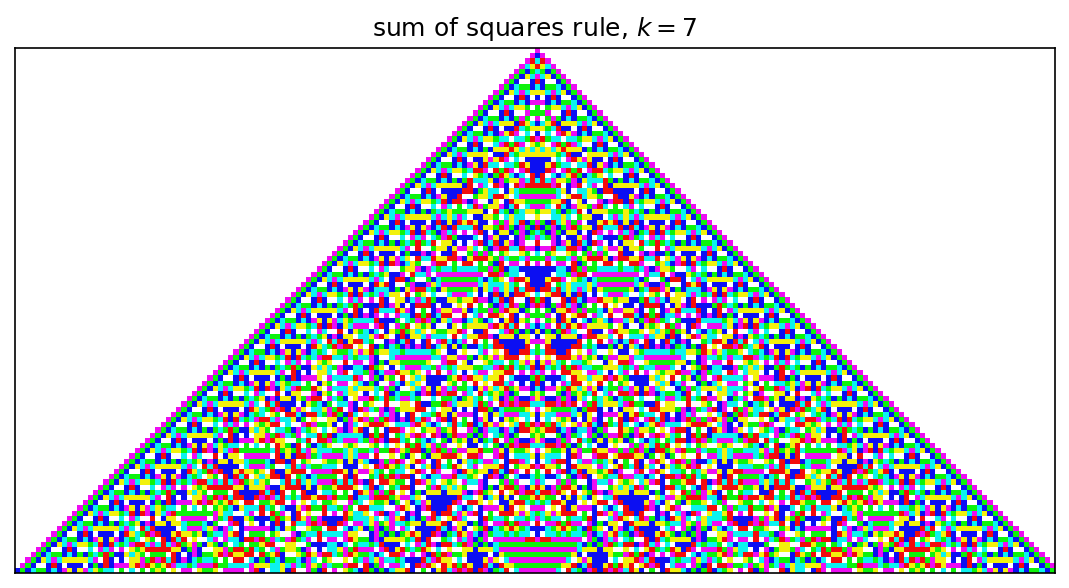
\includegraphics[width=0.42\textwidth]{ch3_sumsq_k7}\;
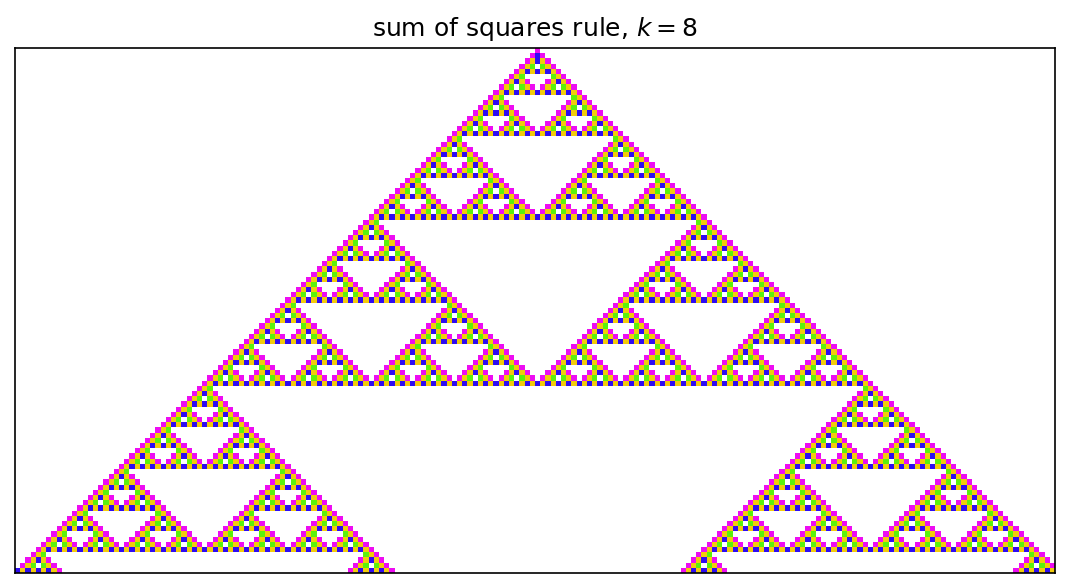
\includegraphics[width=0.42\textwidth]{ch3_sumsq_k8}\\[0.5ex]
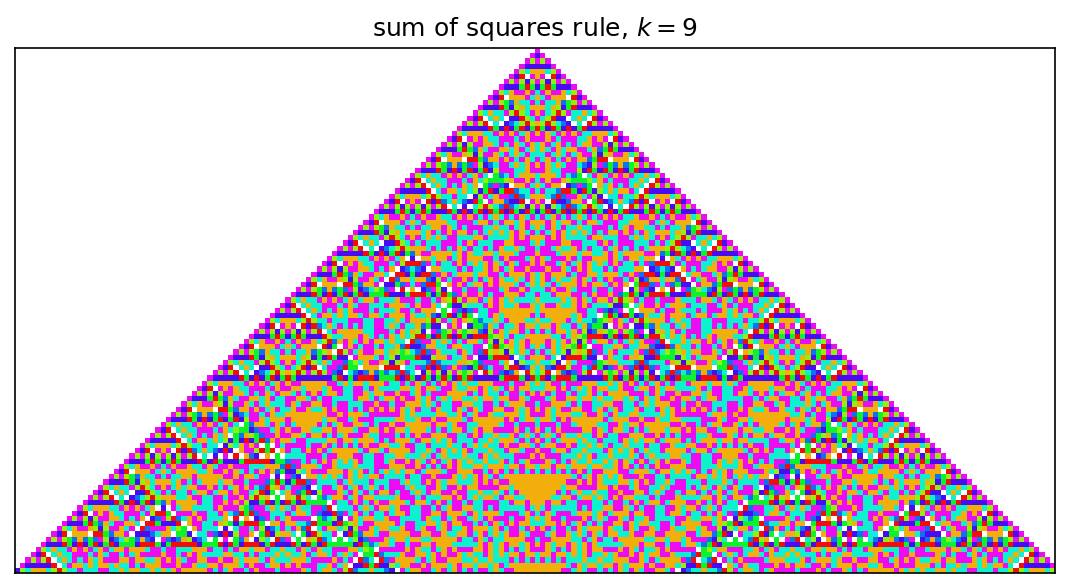
\includegraphics[width=0.42\textwidth]{ch3_sumsq_k9}\;
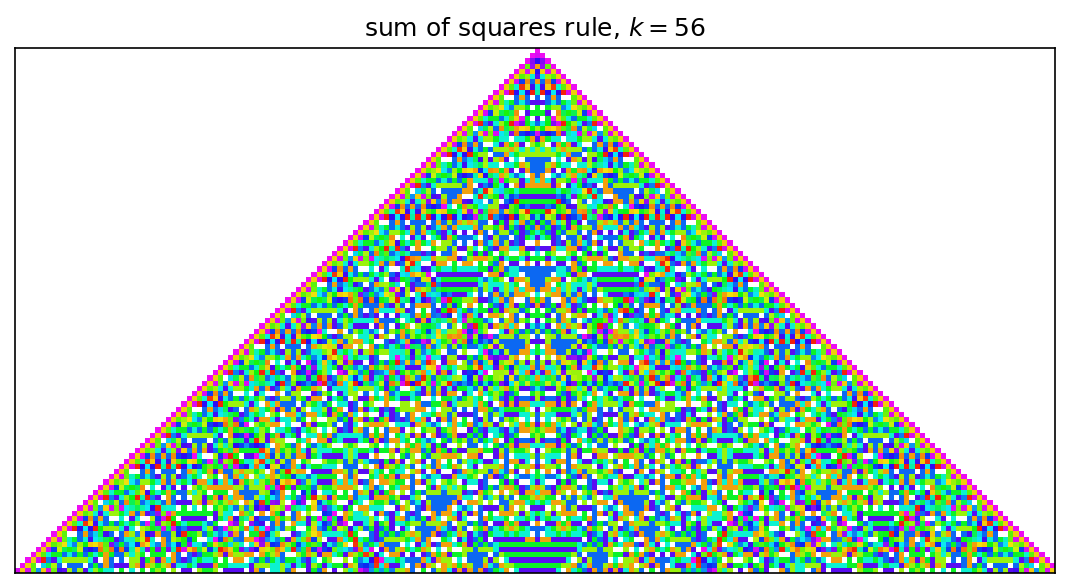
\includegraphics[width=0.42\textwidth]{ch3_sumsq_k56}\\[0.5ex]
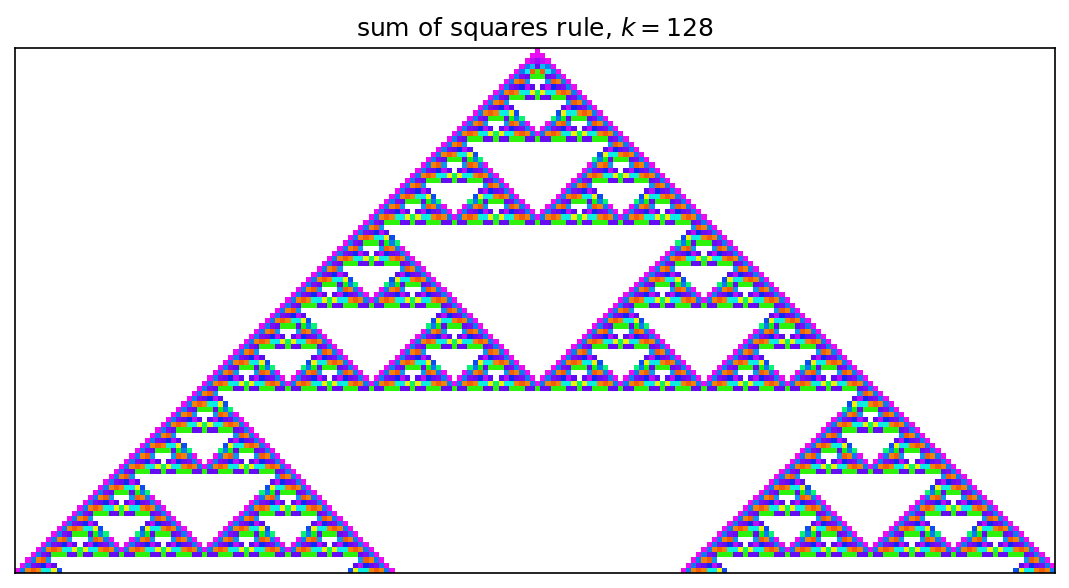
\includegraphics[width=0.42\textwidth]{ch3_sumsq_k128}
\caption{The sum-of-squares rule, 100 generations, for moduli
$k = 7,\ 8=2^3,\ 9,\ 56,\ 128=2^7$.}
\label{fig:sumsq}
\end{figure}

\section{Wolfram's Elementary Cellular Automata}
\label{sec:elementary}

The additive rules above are a small corner of a famous finite family.
Fix $k=2$ and let each cell's neighborhood be itself together with its
immediate left and right neighbors.  A transition rule must assign an
output bit to each of the $2^3 = 8$ possible neighborhood patterns, so
there are exactly $2^8 = 256$ such rules.  Following Wolfram, we number
them: writing the eight outputs for the neighborhoods
$111, 110, 101, \dots, 000$ as a binary string and reading it as a
number from 0 to 255 gives the \emph{rule number}.  These 256
\emph{elementary cellular automata} are the simplest nontrivial CA, and
despite their austerity they already exhibit the full range of
qualitative behavior catalogued in Chapter~6.

Several are old friends.  The additive rule $[1\;0\;1]$ mod 2 of
Section~\ref{sec:kernel101} --- the Sierpi\'nski rule --- is exactly
\textbf{Rule 90}: $C^{(t+1)}_i = C^{(t)}_{i-1} \oplus C^{(t)}_{i+1}$.
The neighborhood-sum rule $[1\;1\;1]$ mod 2 is \textbf{Rule 150}.  But
most elementary rules are \emph{not} additive, and two in particular
have become famous.  \textbf{Rule 30},
\[
  C^{(t+1)}_i = C^{(t)}_{i-1} \oplus
                \bigl(C^{(t)}_i \vee C^{(t)}_{i+1}\bigr),
\]
generates from a single seed a pattern so statistically random-looking
that its center column was used as a random-number generator in early
versions of \emph{Mathematica}; yet it is completely deterministic and
its left edge is perfectly regular (Figure~\ref{fig:rule30}).
\textbf{Rule 110}, discussed further in Chapter~6, supports moving
particle-like structures that interact in complicated ways and was
eventually proved capable of universal computation.

\begin{figure}[htbp]\centering
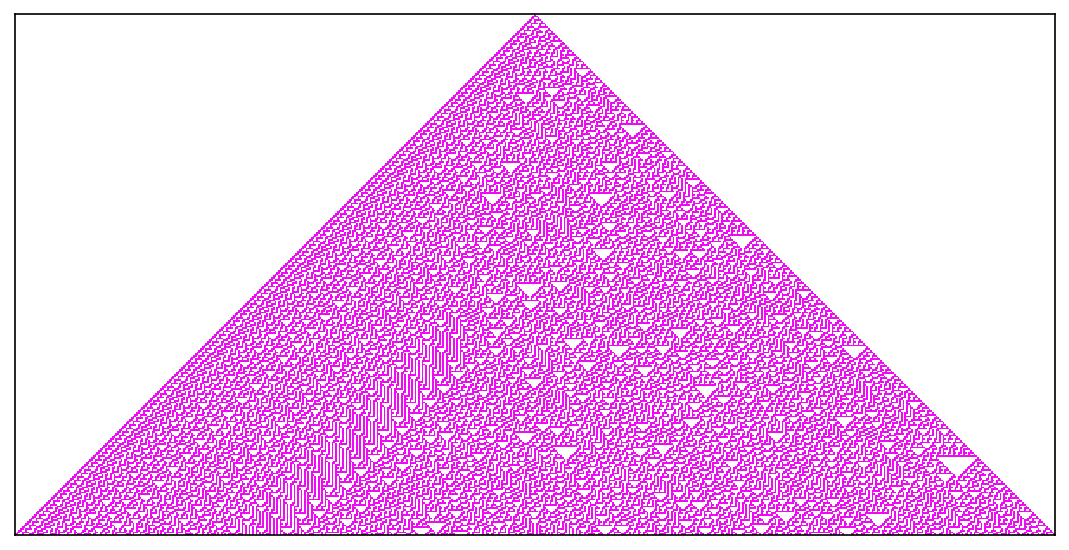
\includegraphics[width=0.8\textwidth]{ch3_rule30}
\caption{Rule 30 evolved from a single seed.  The regular left half and
chaotic right half coexist in a fully deterministic rule; the central
column passes many tests for randomness.}
\label{fig:rule30}
\end{figure}

The module \texttt{cadyn.ca1d} implements all 256 rules through a single
function:

\begin{lstlisting}
from cadyn import ca1d

# Rule 90 reproduces the Sierpinski gasket of Section 3.4
hist = ca1d.run_elementary(ca1d.single_seed(512), rule=90,
                           generations=255)
ca1d.plot_spacetime(hist, k=2)

# Rule 30's pseudo-random central column
hist = ca1d.run_elementary(ca1d.single_seed(601), rule=30,
                           generations=300)
bits = hist[:, 300]          # the center column, one bit per generation
\end{lstlisting}

Figure~\ref{fig:elemclasses} shows one representative of each of
Wolfram's four qualitative classes.  We return to this classification,
and to the surprising depth hidden in Rule 110, in Chapter~6.

\begin{figure}[htbp]\centering
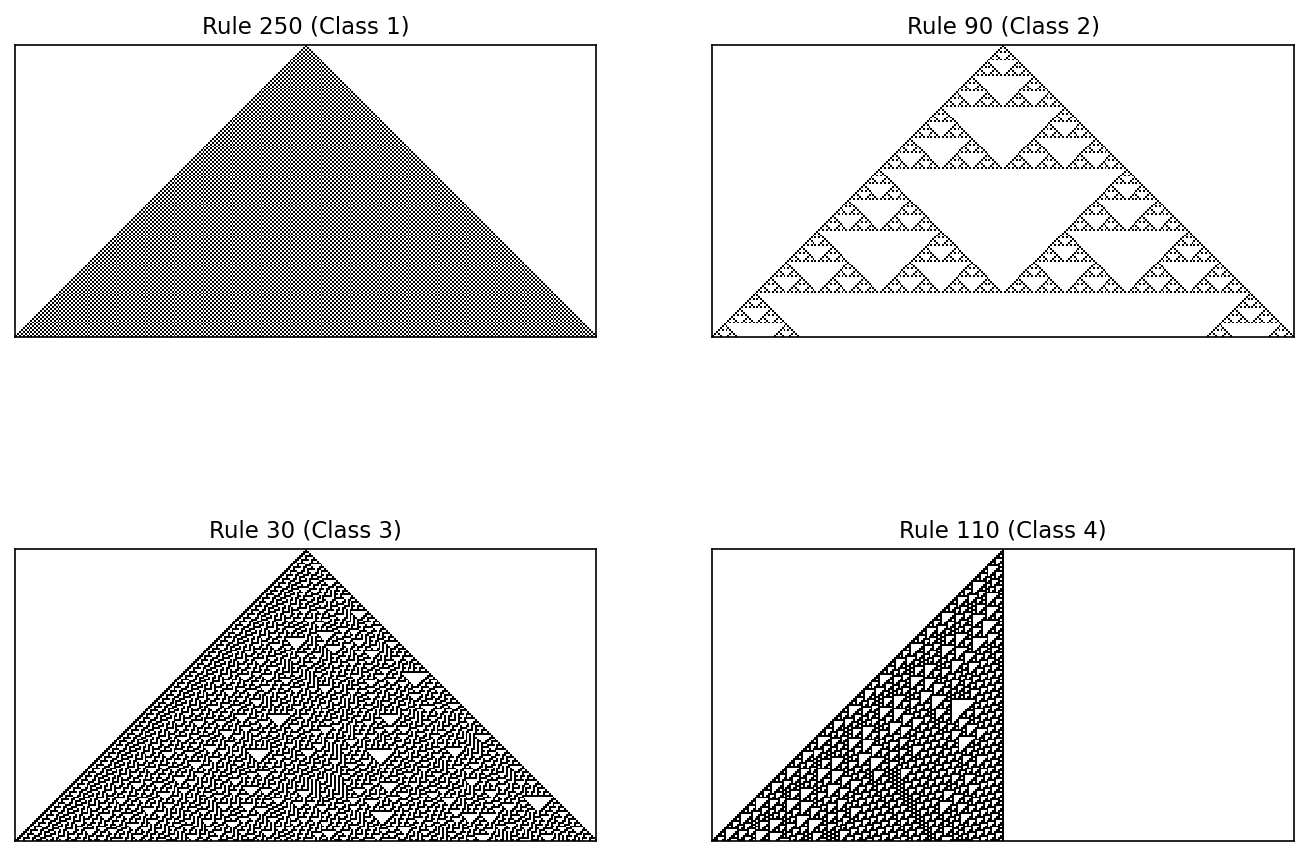
\includegraphics[width=\textwidth]{ch3_elementary_classes}
\caption{Four elementary rules, one per Wolfram class: Rule 250
(Class~1, uniform growth), Rule 90 (Class~2, self-similar), Rule 30
(Class~3, chaotic), Rule 110 (Class~4, complex).}
\label{fig:elemclasses}
\end{figure}

\section{A Strange Non-Additive Example: $k=256$, $n=512$}
\label{sec:life1d}

We now examine a rather bizarre non-additive CA.  Although constructed
with 256 states, its essential behavior requires only 2: the other 254
states exist primarily to add color, so consider any color ``alive''
and white ``dead.''  Let $L$ be the number of live cells in the set
\begin{equation}
  \bigl\{\, C^{(t)}_{i-4},\ C^{(t)}_{i-3},\ C^{(t)}_{i-1},\
            C^{(t)}_{i+1},\ C^{(t)}_{i+3},\ C^{(t)}_{i+4} \,\bigr\}.
\end{equation}
Then
\begin{equation}
  C^{(t+1)}_i =
  \begin{cases}
    \text{alive}, & \text{if } L = 3;\\
    \text{alive}, & \text{if } L = 2 \text{ and } C^{(t)}_i
                    \text{ is alive};\\
    \text{dead}, & \text{otherwise}.
  \end{cases}
\end{equation}
This strange rule is a 1-dimensional version of the 2-dimensional CA
discussed in Section~\ref{sec:gameoflife}.  For the run of
Figure~\ref{fig:life1d} the initial configuration assigned life and
death at random with probability of life $1/2$.  Sections of such runs
look amazingly like elementary-particle tracks in a bubble chamber:
persistent ``particles'' travel at constant velocity, collide,
annihilate, and occasionally settle into small cycling structures.

\begin{figure}[htbp]\centering
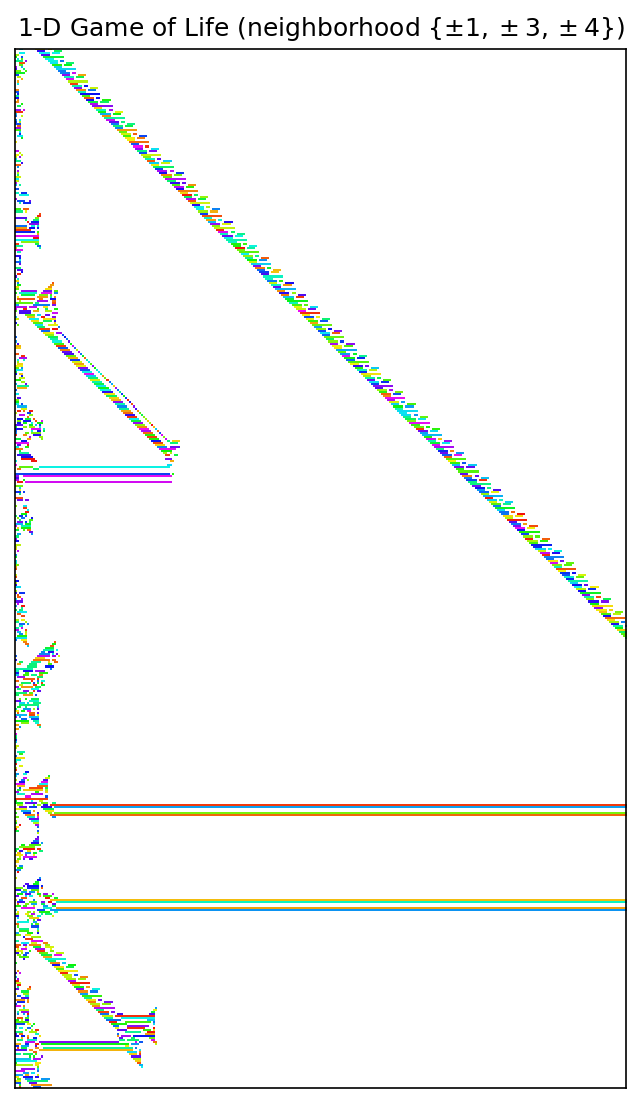
\includegraphics[width=\textwidth]{ch3_life1d}
\caption{A 1-dimensional version of the Game of Life; time increases
left to right.}
\label{fig:life1d}
\end{figure}

\section{Entropy in One Dimension}
\label{sec:entropy1d}

Section~\ref{sec:k5n21} asserted that most CA exhibit decreasing
Shannon entropy as time proceeds, as in the 0-dimensional case.  We can
now make that claim quantitative.  A natural extension of the entropy
of Section~\ref{sec:entropy} to one dimension is the \emph{spatial
entropy} of a single generation: with $p_t(v)$ the fraction of the $n$
cells holding value $v$ at time $t$,
\begin{equation}
  H_t \;=\; -\sum_{v=0}^{k-1} p_t(v)\,\log_2 p_t(v),
\end{equation}
which is $0$ for a uniform state and $\log_2 k$ when all $k$ values
are equally common across the lattice.\footnote{Spatial entropy
measures the diversity of cell values in one configuration.  It is the
simplest of a family of entropies for CA; the \emph{set entropy} over
the ensemble of reachable configurations, and block entropies over
words of length $\ell$, refine it and figure prominently in Wolfram's
analyses.}

Figure~\ref{fig:entropy1d} tracks $H_t$ for four rules of this
chapter, each started (where meaningful) from the same random initial
state with $k=8$ and $n=400$.  The freezing rule $f\equiv0$ collapses
to zero entropy in one step --- the 1-dimensional analogue of the
zero-entropy example of Section~\ref{sec:entropy}.  The additive rule
$[1\;1\;1]$ and the non-additive sum-of-squares rule hover near the
maximum $\log_2 8 = 3$ bits: they scramble values thoroughly enough to
keep the lattice population near-uniform.  The 1-dimensional Life of
Section~\ref{sec:life1d} settles between the extremes: its dynamics
thin the initial random soup down to a sparse population of particles
against a dead background, and the entropy declines accordingly before
leveling off.  Determinism forbids the \emph{basin-of-attraction}
entropy of the ensemble from ever increasing; the spatial entropy of a
typical trajectory usually (though not invariably) declines as
structure emerges.

\begin{figure}[htbp]\centering
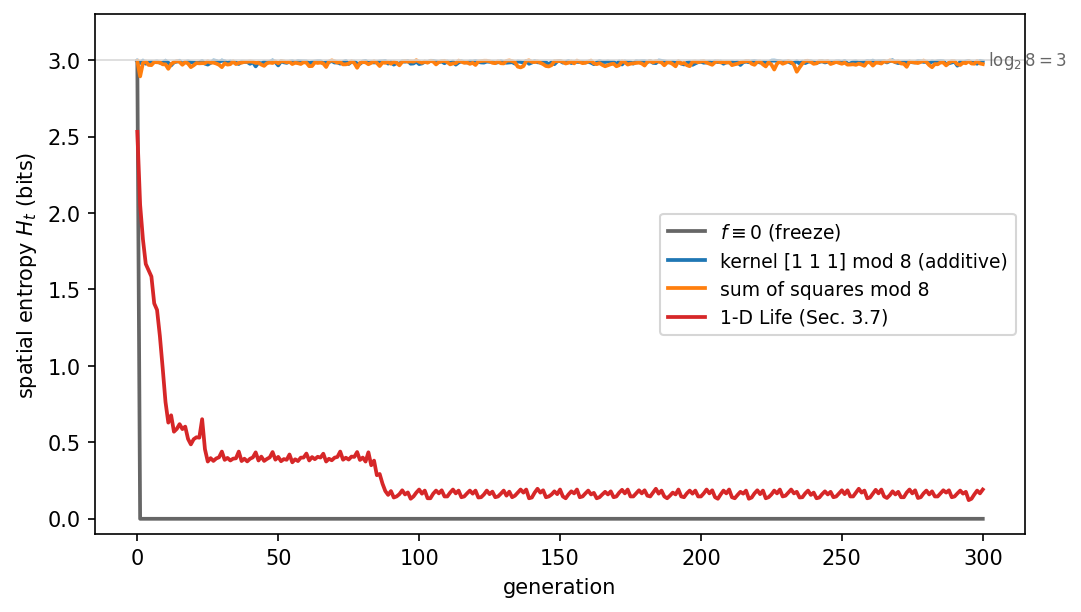
\includegraphics[width=0.85\textwidth]{ch3_entropy_comparison}
\caption{Spatial entropy versus time for four rules with $k=8$,
$n=400$, from a random initial state.}
\label{fig:entropy1d}
\end{figure}

\chapter{2-Dimensional Cellular Automata}

\section{Preliminaries}

A 2-dimensional lattice is an array of cells tiling an infinite planar
surface, each taking a value from a finite set at each tick of the
clock; the state at time $t$ is the doubly infinite array
$C^{(t)} = \bigl[\,C^{(t)}_{ij}\,\bigr]$.  As before we consider only
periodic boundary conditions, but now the wrap-around occurs in two
directions: right wraps to left and bottom wraps to top.  Fixing $n$
rows and $m$ columns, the state becomes the finite array
\begin{equation}
  C^{(t)} =
  \begin{bmatrix}
    C^{(t)}_{0,0} & C^{(t)}_{0,1} & \cdots & C^{(t)}_{0,m-1}\\
    C^{(t)}_{1,0} & C^{(t)}_{1,1} & \cdots & C^{(t)}_{1,m-1}\\
    \vdots & \vdots & \ddots & \vdots\\
    C^{(t)}_{n-1,0} & C^{(t)}_{n-1,1} & \cdots & C^{(t)}_{n-1,m-1}
  \end{bmatrix}.
\end{equation}
One way to visualize the periodic boundary condition: join the top and
bottom of the array to form a tube, then join the ends of the tube.
Our lattice has the topology of a \emph{torus}.  Equivalently, tile the
infinite plane with copies of the $n\times m$ array, requiring
\begin{equation}
  a \equiv b \pmod n,\ \ c \equiv d \pmod m
  \;\Longrightarrow\; C^{(t)}_{a,c} = C^{(t)}_{b,d}:
\end{equation}
all arithmetic on the first index is done modulo $n$, on the second
modulo $m$.

As before, we consider homogeneous CA (the same relative neighborhood
for every cell), let $k$ denote the number of states, identified with
$0,1,\dots,k-1$, and compute cell values modulo $k$.  The number of
possible states of such a CA is $k^{nm}$; in
Section~\ref{sec:vonneumann}, with $k=256$
and $n=m=500$, the number of states is $256^{500\cdot500} >
10^{602059}$.

Before the examples we discuss the generalization of the convolution
kernels found so useful in the previous chapter.  These 2-dimensional
kernels are used extensively in image processing.

\section{2-Dimensional Convolution Kernels}

One of the most frequently used procedures in image processing is
filtering an image by convolving it with a 2-dimensional kernel.  The
procedure closely parallels the 1-dimensional case.  For example, the
kernel
\[
  \begin{bmatrix*}[r] 0 & -1 & 0\\ -1 & 4 & -1\\ 0 & -1 & 0
  \end{bmatrix*}
\]
applied to a digital image serves as an \emph{edge extractor}, since it
maps homogeneous regions to zero.  Center the kernel over each pixel
and form the multiply-and-add.  For the image fragment
\[
  \begin{bmatrix} 1 & 2 & 3\\ 5 & \mathbf{6} & 7\\ 8 & 9 & 1
  \end{bmatrix}
\]
the output value at the central pixel (input value 6) is
\[
  0\cdot1 + (-1)\cdot2 + 0\cdot3
  + (-1)\cdot5 + 4\cdot6 + (-1)\cdot7
  + 0\cdot8 + (-1)\cdot9 + 0\cdot1 = 1 .
\]
In general, for an $N\times M$ image $x_{ij}$ and a
$(2Q\!-\!1)\times(2Q\!-\!1)$ kernel $k_{fh}$, the output with periodic
boundaries is
\begin{equation}
  y_{ij} \;=\; \sum_{f=1-Q}^{Q-1}\ \sum_{h=1-Q}^{Q-1}
     k_{fh}\; x_{(i+f)\bmod N,\ (j+h)\bmod M}.
\end{equation}
Additive 2-dimensional CA are amenable to detailed mathematical
analysis and admit a polynomial representation similar to the
1-dimensional case, but with two variables
(Section~\ref{sec:poly2d}).

\section{Interlude: The Same Kernels as Image Filters}
\label{sec:imageproc}

Before returning to CA proper it is worth pausing to actually
\emph{see} the image-processing use of this machinery, since the two
computations are literally identical: one generation of an additive CA
is one convolution pass over an image, minus the mod-$k$ reduction.
Figure~\ref{fig:imageproc} applies two kernels from this chapter to a
synthetic grayscale test image (a gradient background bearing a disk, a
square, and a triangle, with mild noise).

The center panel shows a single pass of the edge-extracting Laplacian
kernel introduced in the previous section: homogeneous regions ---
where a pixel equals the average
of its four neighbors --- are mapped to zero, so only the boundaries of
the shapes survive.  The right panel shows six iterated passes of the
smoothing kernel
\[
  \tfrac{1}{16}
  \begin{bmatrix} 1&2&1\\ 2&4&2\\ 1&2&1 \end{bmatrix},
\]
the outer product $[1\;2\;1]^{\mathsf T}[1\;2\;1]$ of the very kernel
used in the worked example of Section~3.1, normalized to sum to 1.
Iterating a smoothing convolution is running a CA whose long-run
behavior is the diffusion (heat) equation --- a first concrete instance
of the claim of Chapter~1 that CA yield discrete approximations to
differential equations.  Where an image processor stops after one or a
few passes, a CA keeps going; the difference between the two fields is,
as promised, one of intent rather than mechanism.

\begin{figure}[htbp]\centering
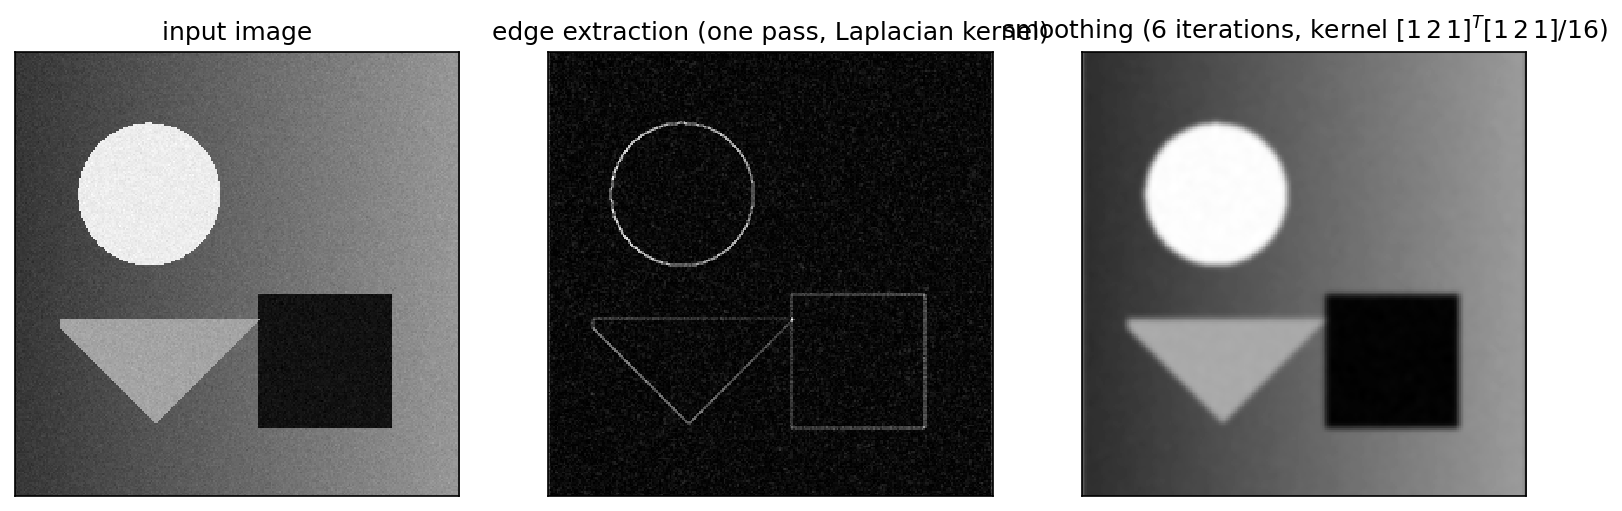
\includegraphics[width=\textwidth]{ch4_image_processing}
\caption{The kernels of this chapter doing their day job.  Left: a
synthetic test image.  Center: one pass of the Laplacian
edge-extraction kernel (absolute value shown).  Right: six passes of
the normalized smoothing kernel --- iterated convolution as discrete
diffusion.}
\label{fig:imageproc}
\end{figure}

\section{Example: $k=256$, $n=m=500$, the von Neumann kernel}
\label{sec:vonneumann}

For this example the state at generation $t$ is a $500\times500$ array
with entries in $\{0,\dots,255\}$; wrap-around is imposed by modulo-500
arithmetic on the indices.  The neighborhood of a cell is the cell
itself with its left, right, upper, and lower neighbors, and the rule
is the neighborhood sum modulo 256:
\begin{equation}
  C^{(t+1)}_{ij} = C^{(t)}_{i,j-1} + C^{(t)}_{i-1,j} + C^{(t)}_{ij}
  + C^{(t)}_{i,j+1} + C^{(t)}_{i+1,j} \pmod{256},
\end{equation}
compactly expressed by the kernel
\begin{equation}
  \begin{bmatrix} 0&1&0\\ 1&1&1\\ 0&1&0 \end{bmatrix}.
\end{equation}
We start from the simplest initial state: all cells zero except one
cell of value 1.  In the following images black represents zero and
colors the other 255 states.

From this simple seed an ever-growing mandala of intricate complexity
and symmetry unfolds (growing up to the limiting $500\times500$
dimensions of the space).  Figure~\ref{fig:vn} shows the seed after 100
and after 250 generations.  Figure~\ref{fig:vnseeds} shows the descent
of a different initial state: 256 seeds with values $0,\dots,255$
arranged on a grid, after 13 generations --- each seed the germ of its
own distinct mandala.  (The seed of value 0 is a perfectly valid seed;
it simply proves infertile, leaving a conspicuous gap in the garden.)

\begin{figure}[htbp]\centering
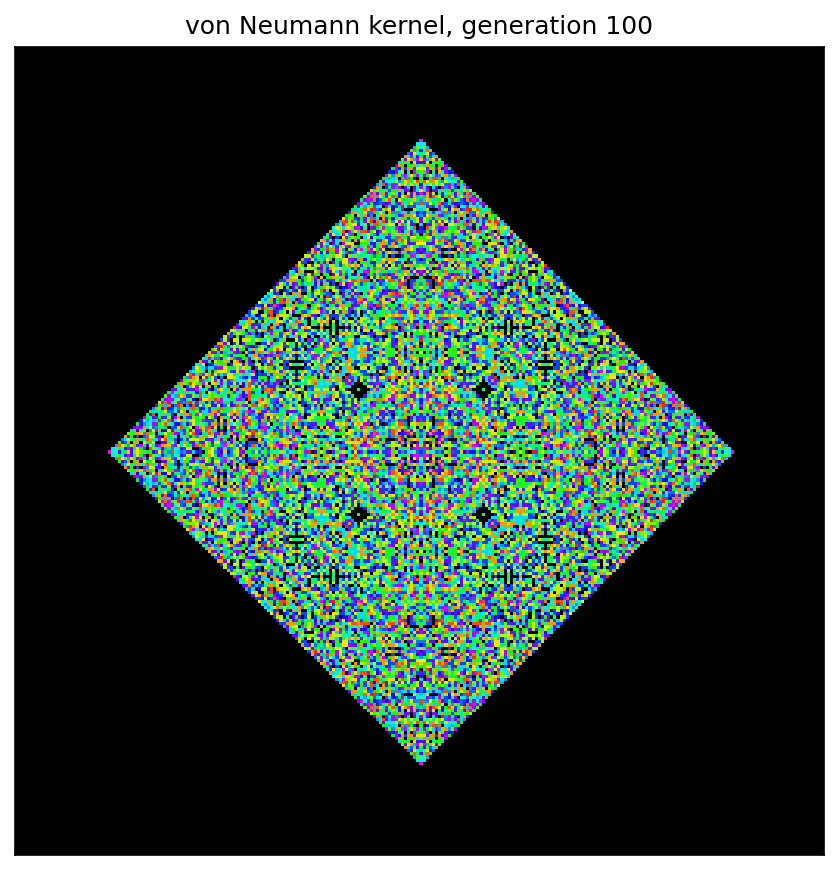
\includegraphics[width=0.48\textwidth]{ch4_vonneumann_gen100}\;
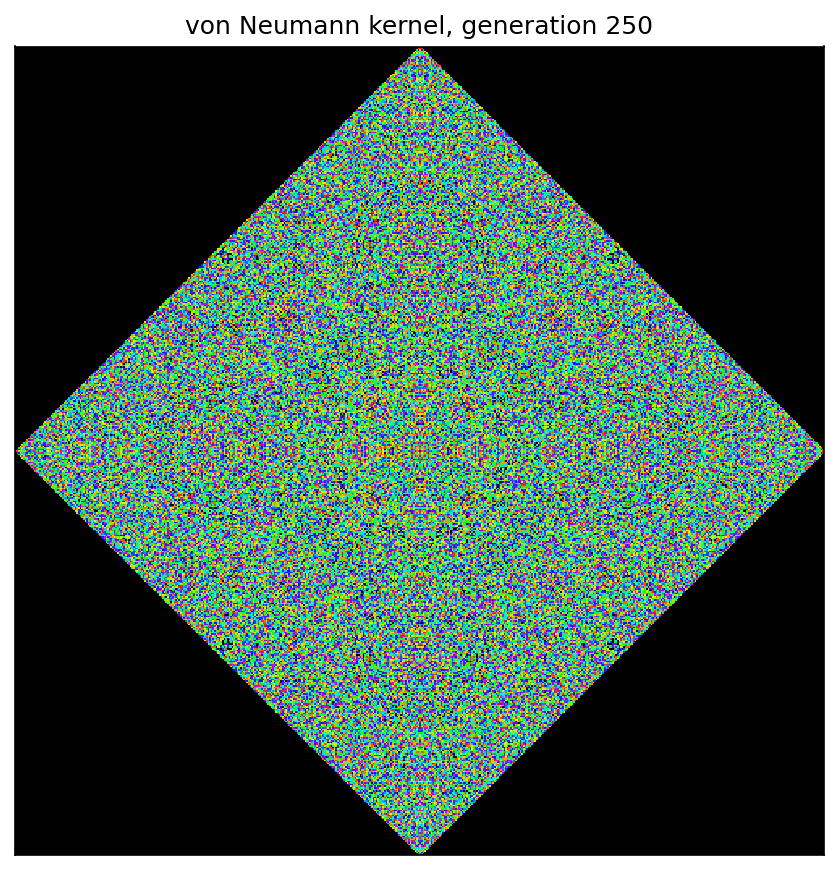
\includegraphics[width=0.48\textwidth]{ch4_vonneumann_gen250}
\caption{The von Neumann--kernel CA grown from a single seed:
generation 100 (detail, left) and generation 250 (right).}
\label{fig:vn}
\end{figure}

\begin{figure}[htbp]\centering
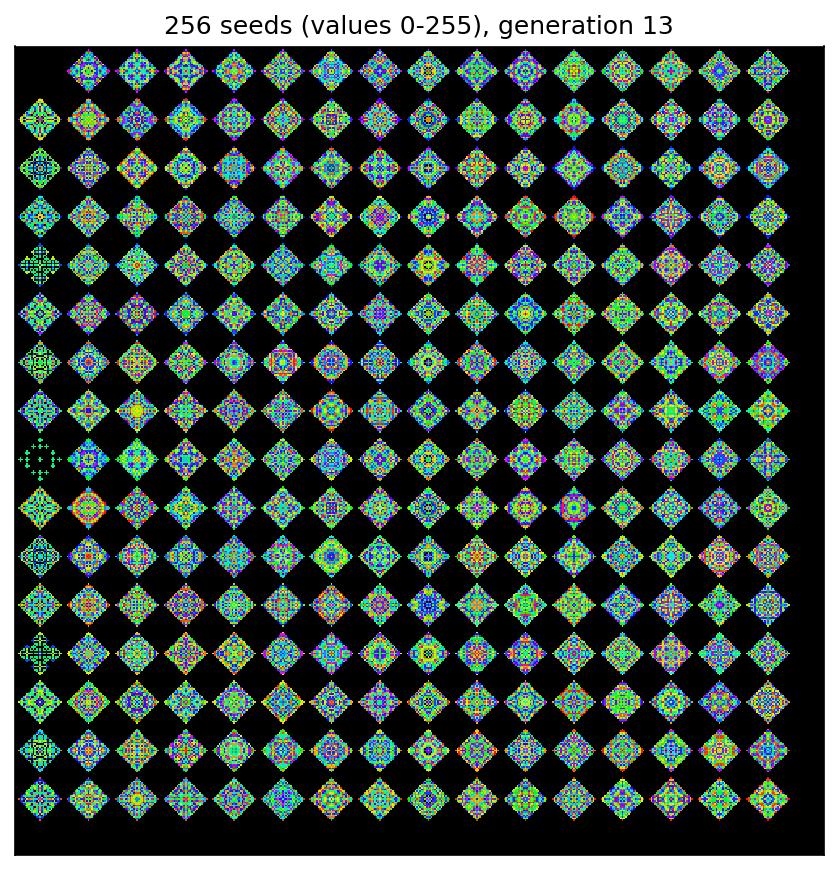
\includegraphics[width=0.7\textwidth]{ch4_vonneumann_seeds_gen13}
\caption{Generation 13 from an initial state of 256 seeds with values
$0,\dots,255$; the value-0 seed, though valid, is infertile.}
\label{fig:vnseeds}
\end{figure}

\section{Example: $k=256$, $n=m=500$, a signed kernel}
\label{sec:kernel43}

With the same lattice and state count as the previous example, we now
take the neighborhood to be the cell together with its eight nearest
neighbors, and the transition rule given by the kernel
\begin{equation}
  \begin{bmatrix*}[r] -1 & 2 & -1\\ 2 & -4 & 2\\ -1 & 2 & -1
  \end{bmatrix*},
\end{equation}
that is,
\begin{equation}
\begin{aligned}
  C^{(t+1)}_{ij} ={}& -C^{(t)}_{i-1,j-1} + 2C^{(t)}_{i-1,j}
                     - C^{(t)}_{i-1,j+1}
                     + 2C^{(t)}_{i,j-1} - 4C^{(t)}_{ij}
                     + 2C^{(t)}_{i,j+1}\\
                   & - C^{(t)}_{i+1,j-1} + 2C^{(t)}_{i+1,j}
                     - C^{(t)}_{i+1,j+1} \pmod{256}.
\end{aligned}
\end{equation}
Starting again from a single seed of value 1 (white now representing
zero), we once more see a mandala of intricate complexity and symmetry
unfold; Figure~\ref{fig:k43} shows generation 250 and a magnified
detail.

\begin{figure}[htbp]\centering
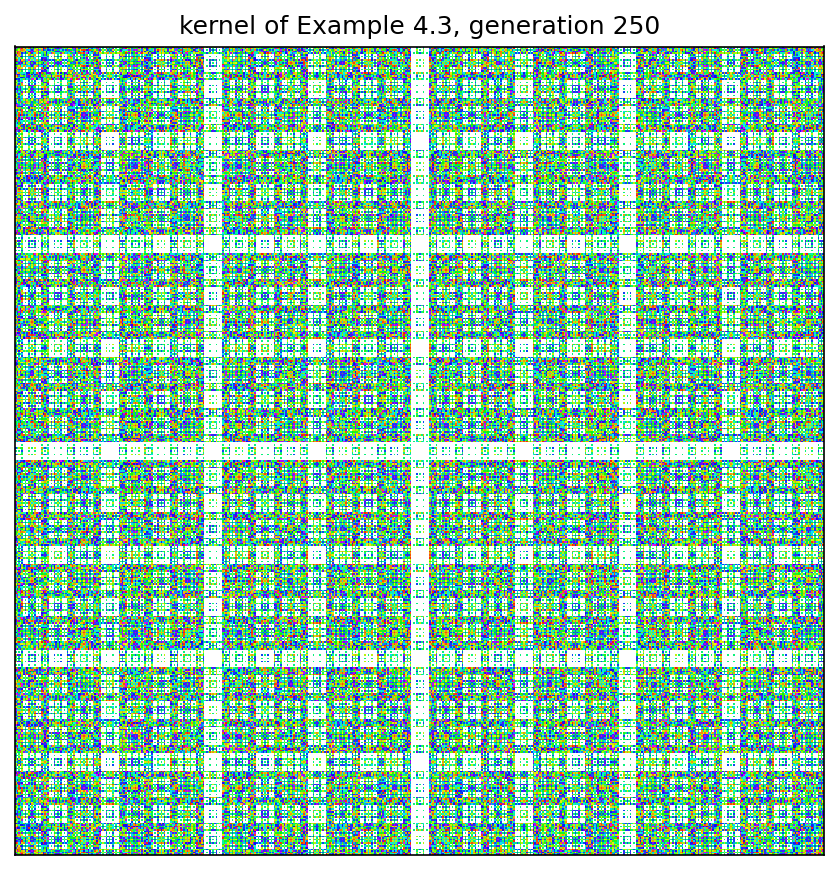
\includegraphics[width=0.48\textwidth]{ch4_kernel43_gen250}\;
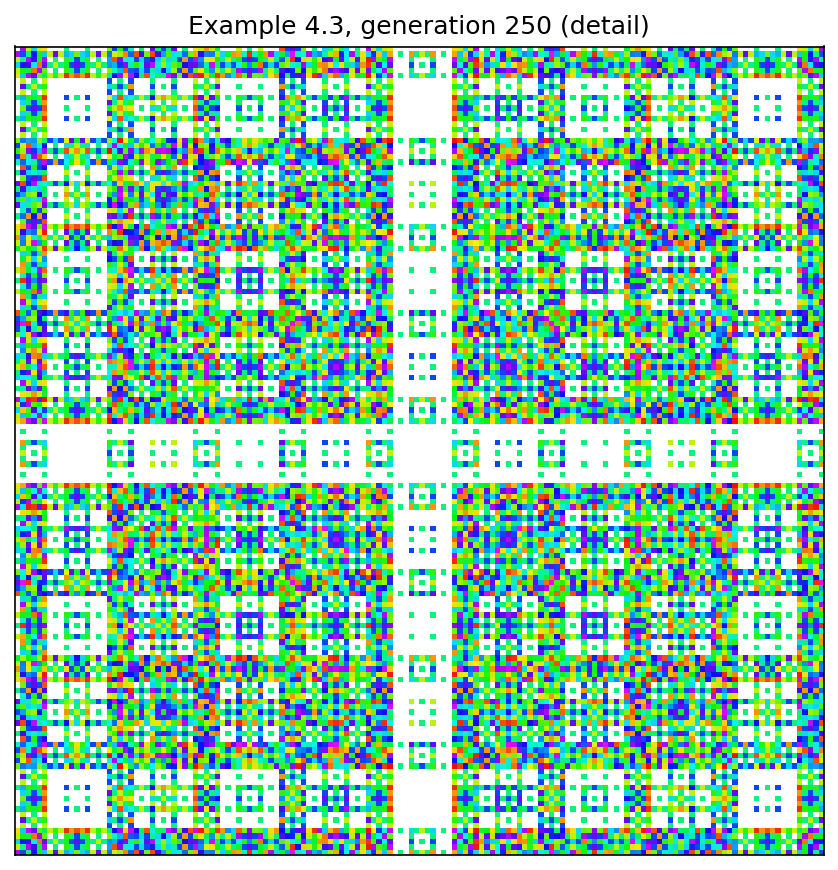
\includegraphics[width=0.48\textwidth]{ch4_kernel43_gen250_detail}
\caption{The signed-kernel CA of Section~\ref{sec:kernel43} at
generation 250 (left) with a magnified central detail (right).}
\label{fig:k43}
\end{figure}

\section{Polynomial Representation of 2-Dimensional Additive CA}
\label{sec:poly2d}

Two-dimensional additive CA have polynomial representations paralleling
Section~\ref{sec:poly1d}.  A state --- an $n\times m$ matrix
$[a_{ij}]$ of integers mod $k$ --- is represented by the two-variable
characteristic polynomial
\begin{equation}
  A(x,y) \;=\; \sum_{i=0}^{n-1}\sum_{j=0}^{m-1} a_{ij}\, x^i y^j ,
\end{equation}
an element of the ring
$\mathbb{Z}_k[x,y]\,/\,(x^n-1,\ y^m-1)$: $x$-exponents are computed
modulo $n$, $y$-exponents modulo $m$, coefficients modulo $k$.  A
kernel translates into a polynomial $T(x,y)$ exactly as before; for
the kernel of Section~\ref{sec:kernel43},
\begin{equation}
\begin{aligned}
  T(x,y) ={}& -x^{-1}y^{-1} + 2x^{-1} - x^{-1}y
             + 2y^{-1} - 4 + 2y
             - xy^{-1} + 2x - xy\\
  \equiv{}& -x^{n-1}y^{m-1} + 2x^{n-1} - x^{n-1}y + 2y^{m-1} - 4 + 2y
            - xy^{m-1} + 2x - xy .
\end{aligned}
\end{equation}
Multiplying $A$ by $T$ yields the next generation.  Though the algebra
grows involved in higher dimensions, the polynomial representation is a
valuable conceptual tool: the superposition principle is simply the
distributive law of polynomial multiplication over addition.
Superposition says, in effect, that if you've seen one cell evolve,
you've seen all possible configurations of cells evolve.

Unfortunately, the most interesting CA are not additive and enjoy no
such superposition property.

\section{A Famous Non-Additive CA: The Game of Life}
\label{sec:gameoflife}

Conway's Game of Life is a simple 2-dimensional CA in which each cell
is either \emph{alive} or \emph{dead}.  Imagining the cells as squares
of a checkerboard, the neighborhood of a cell consists of its eight
neighboring squares (left, right, up, down, and the four diagonals).
The transition rules are:
\begin{itemize}
\item a dead cell becomes alive in the next generation exactly when it
  has exactly three living neighbors (a \emph{birth});
\item a live cell remains alive exactly when it has two or three
  living neighbors (otherwise it dies of loneliness or
  overcrowding).
\end{itemize}

In the Life figures below, white represents dead cells and live cells
are color-coded by age: cerise cells are newborn, red very young,
orange older, yellow older yet, green still older, blue very old, and
violet ancient --- more than 250 generations old.
Figure~\ref{fig:life2d} shows evolution from an initially random state;
after 500 generations the typical menagerie of Life structures has
emerged: stable \emph{still lifes} (blocks, beehives), oscillating
\emph{blinkers}, and the occasional \emph{glider} crawling across the
torus.  Figure~\ref{fig:liferow} shows evolution from a row of 71
initially live cells; the bilateral symmetry of the initial state is
preserved forever, and from generation 200 on, gliders can be seen at
each corner moving outward.

\begin{figure}[htbp]\centering
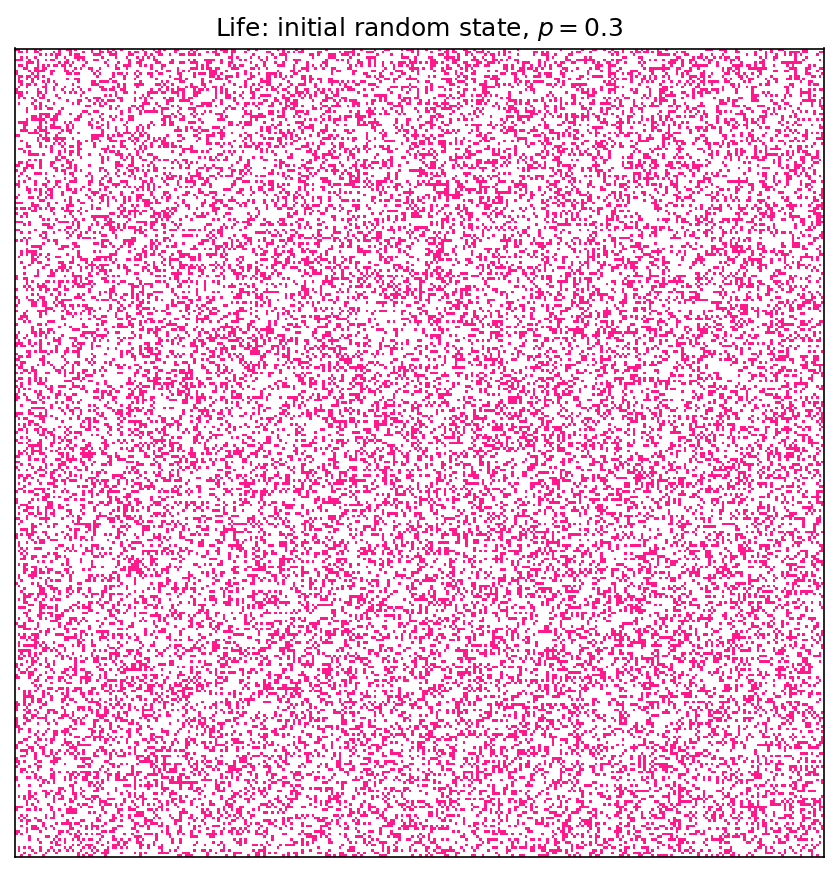
\includegraphics[width=0.48\textwidth]{ch4_life_initial}\;
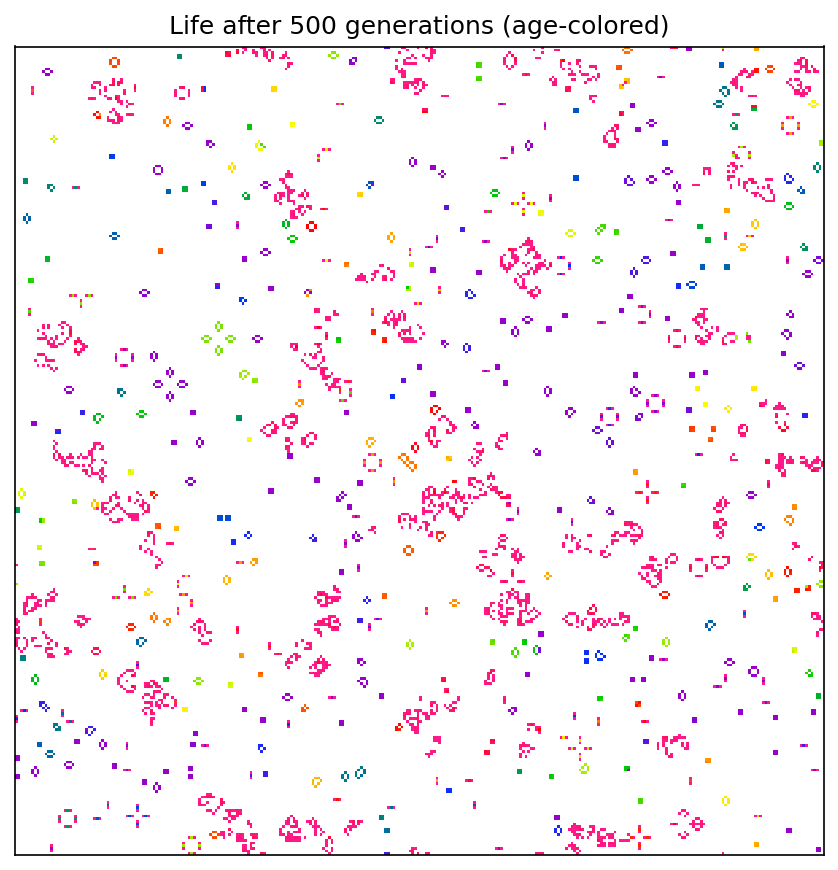
\includegraphics[width=0.48\textwidth]{ch4_life_gen500}
\caption{Life from an initially random state with probability of life
$0.3$ (left); after 500 generations (right), various typical Life
structures have emerged, age-colored.}
\label{fig:life2d}
\end{figure}

\begin{figure}[htbp]\centering
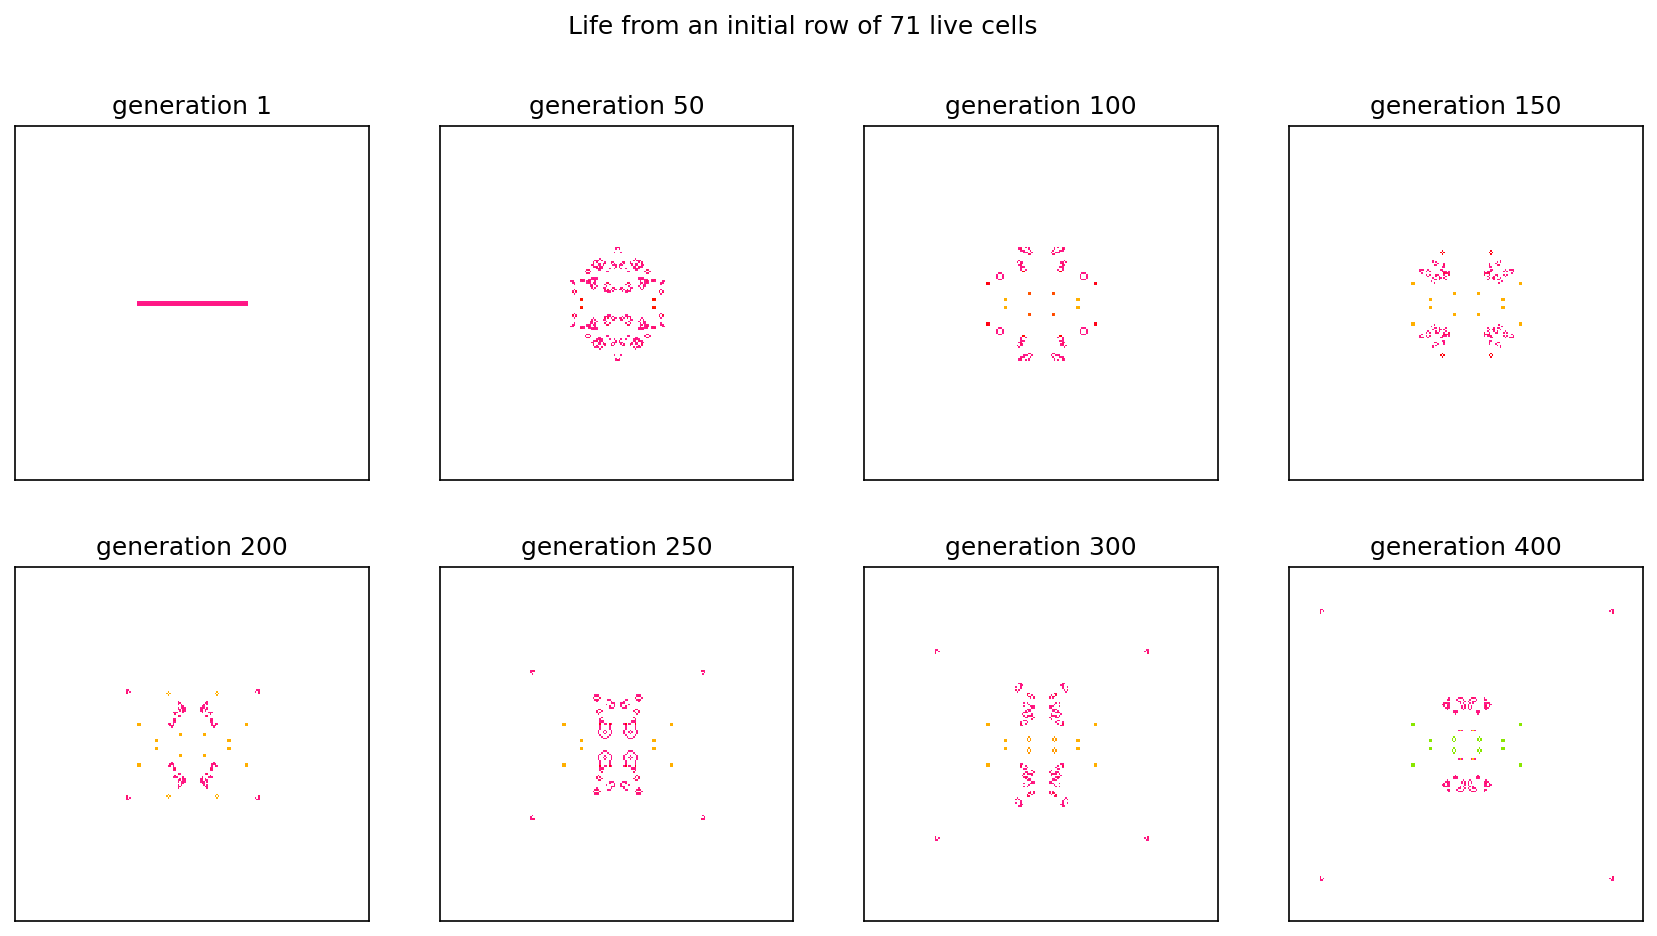
\includegraphics[width=\textwidth]{ch4_life_row71}
\caption{Evolution from an initial row of 71 live cells.}
\label{fig:liferow}
\end{figure}

\expand{Life went on to a remarkable career.  In 1982 Conway and,
independently, Gosper's group established that Life is computationally
universal: glider streams can implement arbitrary logic circuits.
Self-constructing patterns were eventually built explicitly, notably
Gemini (2010), a pattern that constructs a complete copy of itself ---
achieving within Life the self-replication von Neumann originally
sought from cellular spaces.  Conway himself died in April 2020;
Life remains his most famous creation, to his occasional chagrin.}

\subsection*{A small bestiary}

The interest of Life lies in its \emph{structures}.  The simplest are
\emph{still lifes} such as the $2\times2$ block, frozen forever, and
simple oscillators such as the three-in-a-row \emph{blinker}, which
flips between horizontal and vertical with period 2.  Far more
consequential is the \emph{glider} (Figure~\ref{fig:glider}): a
five-cell pattern that, after four generations, reproduces its own
shape displaced one cell diagonally.  Gliders are Life's messengers ---
the moving particles out of which computation is built.

\begin{figure}[htbp]\centering
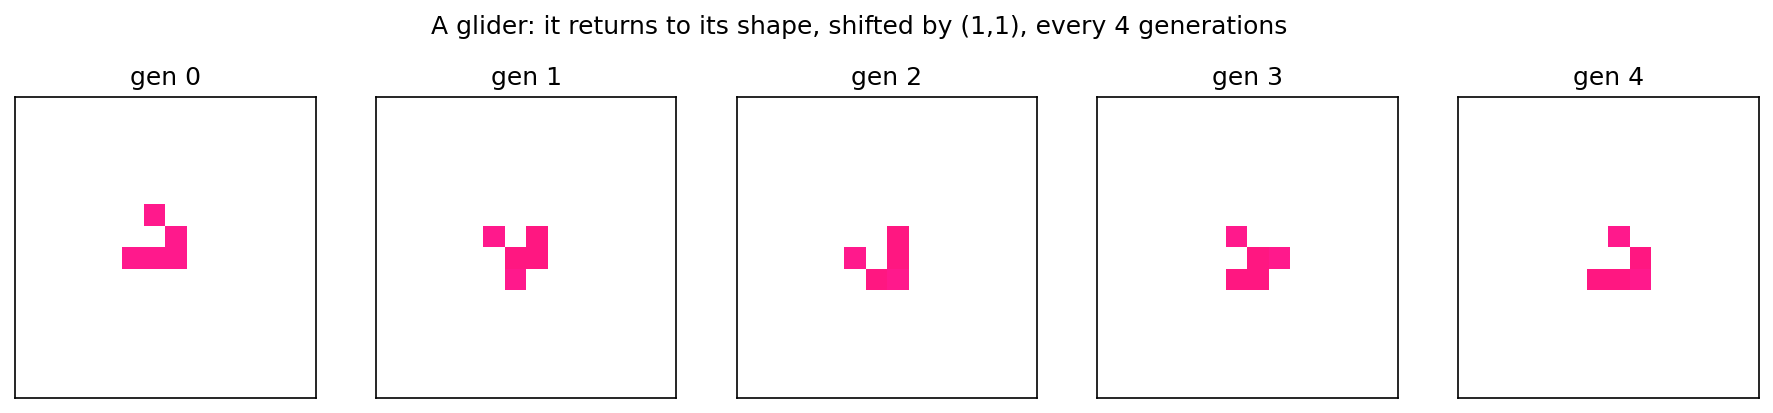
\includegraphics[width=\textwidth]{ch4_glider}
\caption{The glider returns to its original shape, translated by one
cell diagonally, every four generations --- a self-propelled pattern
moving across the torus.}
\label{fig:glider}
\end{figure}

That gliders can be manufactured to order was the key to Life's
universality.  Bill Gosper's \emph{glider gun}
(Figure~\ref{fig:gosper}) is a pattern of period 30 that emits a new
glider every 30 generations, a steady stream marching off toward
infinity.  Because a gun's population grows without bound, its
discovery in 1970 settled a \$50 wager posed by Conway --- whether any
Life pattern could grow forever --- and opened the door to building,
within Life, the logic gates, wires, and memory of a universal
computer.

\begin{figure}[htbp]\centering
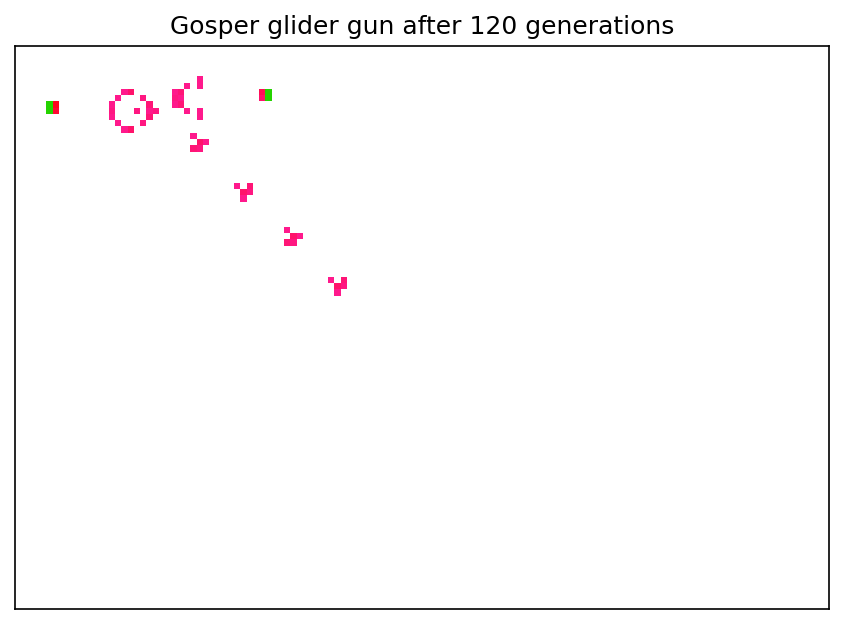
\includegraphics[width=0.75\textwidth]{ch4_gosper_gun}
\caption{Gosper's glider gun after 120 generations: the period-30
mechanism at upper left has emitted a diagonal stream of four gliders.
The population grows without bound.}
\label{fig:gosper}
\end{figure}

The module \texttt{cadyn.ca2d} ships these patterns as data, ready to
place on a torus of any size:

\begin{lstlisting}
from cadyn import ca2d

# a glider in the corner of a 60x60 world, run for 40 generations
grid = ca2d.pattern_grid(ca2d.GLIDER, 60, top=2, left=2)
alive, age = ca2d.run_life(grid, 40)
ca2d.show_life(age)

# the Gosper gun; watch the population climb by 5 cells every 30 gens
gun = ca2d.pattern_grid(ca2d.GOSPER_GLIDER_GUN, 90, 130, top=5, left=5)
alive, age = ca2d.run_life(gun, 120)
\end{lstlisting}

\section{A Non-Additive CA Involving Euler's Totient Function}
\label{sec:totient}

Our second non-additive 2-dimensional example again takes $k=256$ on a
$500\times500$ torus, with the Moore neighborhood (the cell and its
eight nearest neighbors).  The transition rule borrows a function from
number theory, the Euler totient $\varphi$ (Appendix~\ref{app:totient}):
\begin{equation}
  C^{(t+1)}_{ij} \;=\; \sum_{a=-1}^{1}\sum_{b=-1}^{1}
     \varphi\bigl(C^{(t)}_{i+a,\,j+b}\bigr) \pmod{256},
\end{equation}
where we set $\varphi(0)=0$.  Starting from a single seed of value 1
(white $=$ 0), a mandala of intricate complexity and symmetry once more
unfolds; Figure~\ref{fig:totient} shows generation 250 with a
magnified detail.

\begin{figure}[htbp]\centering
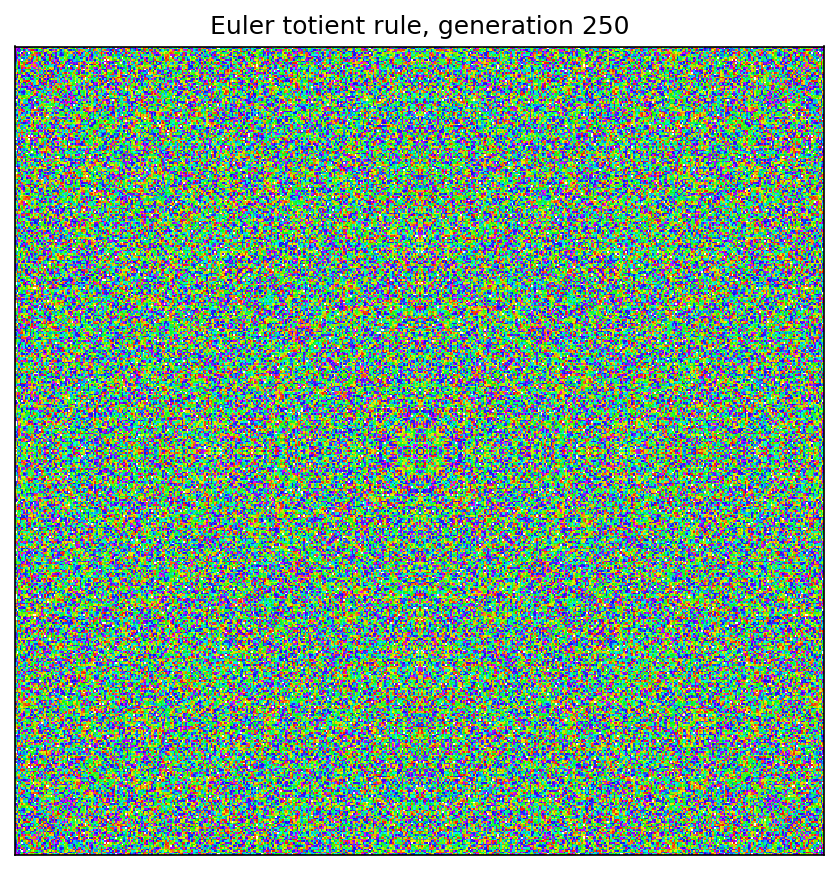
\includegraphics[width=0.48\textwidth]{ch4_totient_gen250}\;
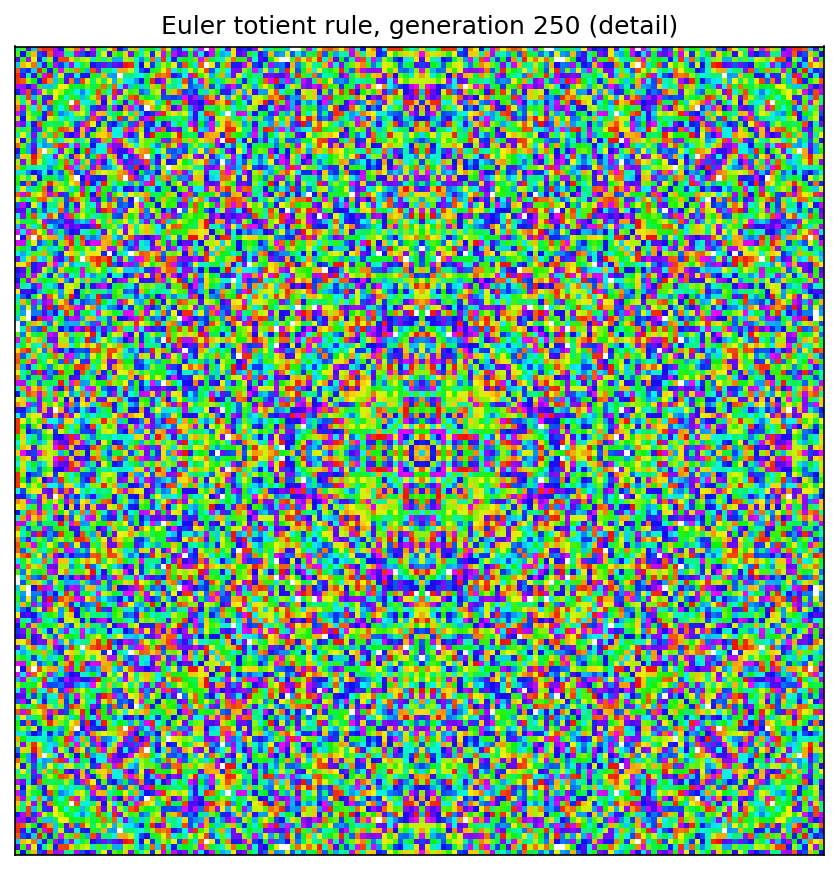
\includegraphics[width=0.48\textwidth]{ch4_totient_gen250_detail}
\caption{The Euler-totient rule at generation 250 (left) and a
magnified central detail (right).}
\label{fig:totient}
\end{figure}

\chapter{Ecosystem Modeling Using Cellular Automata}
\label{ch:ecosystem}

\section{CAecosystem}

The module \texttt{cadyn.ecosystem} illustrates how CA can create
simple, intuitive models of complex real-world phenomena that help
illuminate the underlying principles.  This ecosystem simulator lets
the user set the parameters of an artificial ecosystem with three
interdependent species --- \emph{plants}, \emph{prey}, and
\emph{predators} --- then set the artificial universe in motion,
observe the ensuing dynamics, and display the population data in
various ways.  These created worlds have a toroidal topology: a critter
creeping off the bottom of the display reappears at the top, and one
crawling off the right enters on the left.  So don't worry --- these
critters can't escape and infest your home!

For a first run we use a $500\times500$ cell space with the initial
probability of a cell being prey set to $0.212$ and of being a predator
set to $0.029$; other parameters keep their default settings.
Figure~\ref{fig:eco-init} shows the initial state
(green $=$ plants, yellow $=$ prey, red $=$ predators), and
Figure~\ref{fig:eco-2000} shows the state after 2000 generations
(purple cells are devoid of life).

\begin{figure}[htbp]\centering
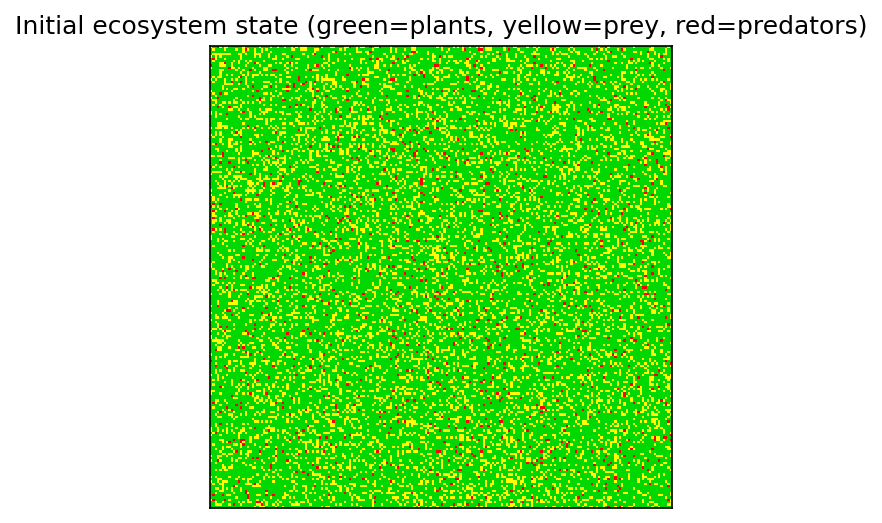
\includegraphics[width=0.7\textwidth]{ch5_eco_initial}
\caption{Initial state of the ecosystem (detail).  Green $=$ plants,
yellow $=$ prey, red $=$ predators.}
\label{fig:eco-init}
\end{figure}

\begin{figure}[htbp]\centering
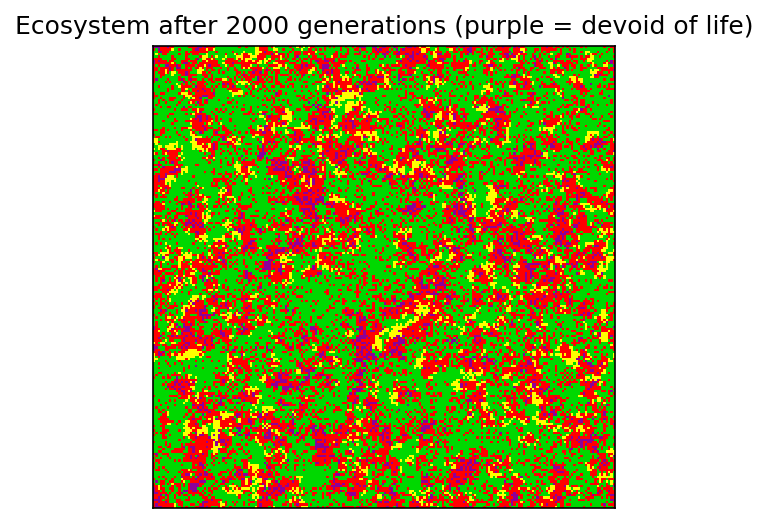
\includegraphics[width=0.7\textwidth]{ch5_eco_gen2000}
\caption{The same ecosystem 2000 generations later (detail); purple
cells are devoid of life.}
\label{fig:eco-2000}
\end{figure}

Figure~\ref{fig:eco-pops} graphs the populations against time, up to
generation 2000.  Without the regulating influence of the predators,
the prey would eat all the plants and then starve.  The three
populations are graphed on a normalized scale for good resolution on a
shared axis.  The predator curve (red) and the prey curve (yellow) show
the out-of-phase oscillation typical of predator/prey systems: abundant
prey mean easy hunting, hence many predator births; the swelling
predator population then drives the prey into decline; scarce prey then
starve the predators; and with predators scarce, the prey rebound,
restarting the cycle.

\begin{figure}[htbp]\centering
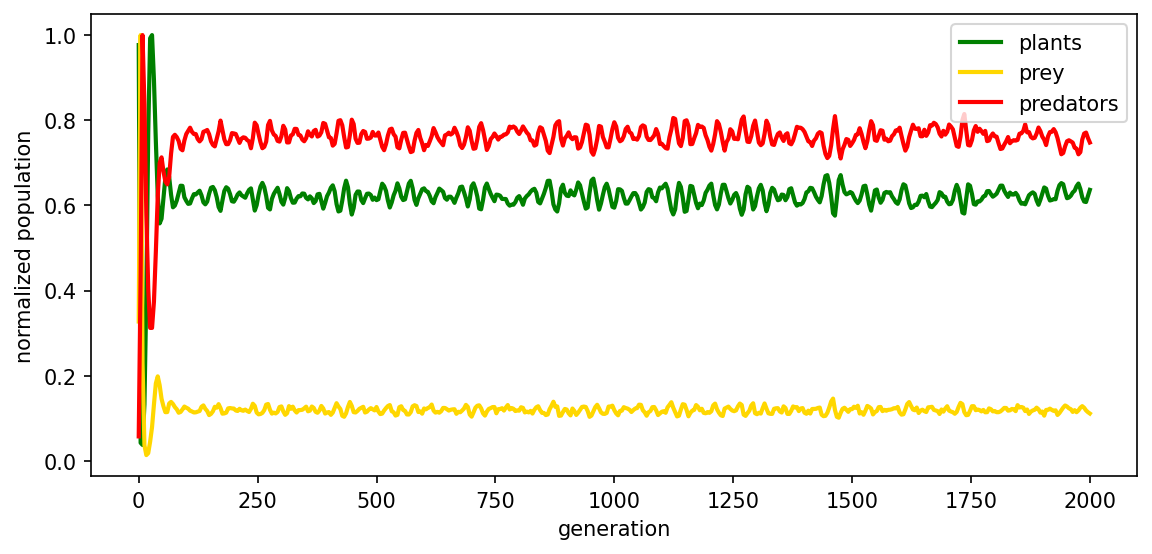
\includegraphics[width=0.9\textwidth]{ch5_eco_populations}
\caption{Normalized population curves; the horizontal axis is the
generation number.}
\label{fig:eco-pops}
\end{figure}

The cycle is less obvious between prey and plants (relative to which the
prey are the predators), because of the rapid growth of plants in this
simulation; the plant graph is almost the negative of the prey graph
(roughly $180^\circ$ out of phase).  Notice that the initially large
oscillations (\emph{transients}) settle to relatively stable
amplitudes for all species, and that the predators and plants stand in
a curiously symbiotic relationship in this ecosystem.

Another view of the same information is the 3-dimensional \emph{phase
portrait}: at each sampled time we plot a point whose coordinates are
the three population counts (Figure~\ref{fig:eco-phase}).  Poincar\'e
introduced this type of graph in his study of the global dynamics of
differential equations.  The oscillation of Figure~\ref{fig:eco-pops}
appears here as an almost circular orbiting of the curve about an
equilibrium point, and the damping of the oscillations appears as a
tightening of the spiral toward that point.

\begin{figure}[htbp]\centering
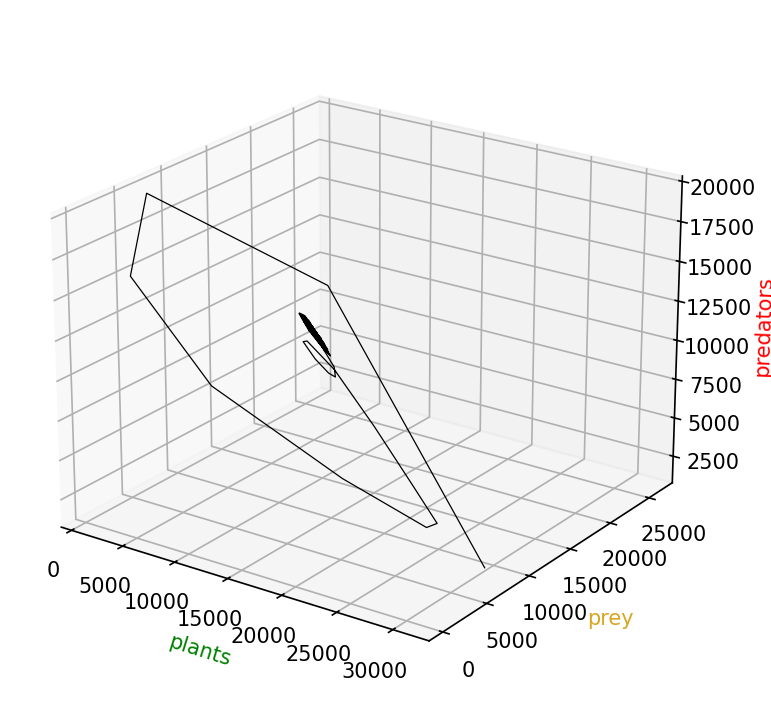
\includegraphics[width=0.7\textwidth]{ch5_eco_phase}
\caption{A 3-dimensional phase portrait representing the same data as
Figure~\ref{fig:eco-pops}: plants ($x$), prey ($y$), predators
($z$).}
\label{fig:eco-phase}
\end{figure}

This same qualitative behavior appears in solutions of the
Volterra--Lotka differential equations traditionally used to model
ecosystem population dynamics.  A little experimentation reveals that an
imprudent choice of parameters produces transients so wild that all
animal life (often all plant life too) goes extinct.
Figure~\ref{fig:extinction} shows such a run: with voracious,
short-lived predators (high predation efficiency, high death rate), the
first predator boom overshoots so violently that it eats the prey
faster than the prey can be replenished, and having exhausted its food
supply the predator population crashes to zero.  Once an animal species
is gone it cannot return --- there is no spontaneous generation in this
model --- so the extinction is permanent.  Even in the
differential-equation models the equilibrium point is virtually
impossible to attain, since it would almost always entail fractions of
an animal being alive --- one of the absurdities of using continuous
models for discrete phenomena.  The difficulty is even more acute in
discrete models, so oscillatory behavior is unavoidable.

\begin{figure}[htbp]\centering
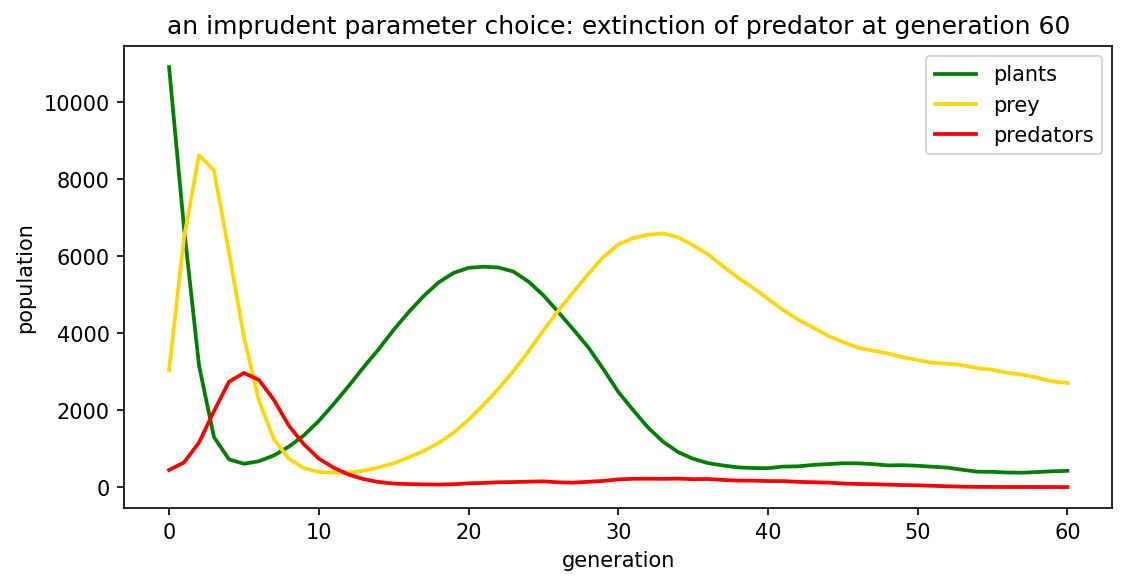
\includegraphics[width=0.85\textwidth]{ch5_extinction}
\caption{An imprudent parameter choice: with predators too efficient
and too short-lived, the first boom-and-bust transient drives the
predators (and here the prey) extinct within the first hundred
generations.}
\label{fig:extinction}
\end{figure}

Which parameter regimes permit long-term coexistence, and which lead to
collapse?  Because the model is stochastic and cheap to run, we can map
this out directly rather than analyze it.  Figure~\ref{fig:survival}
sweeps two predator parameters --- predation efficiency
$b_{\mathrm{pred}}$ and death rate $d_{\mathrm{pred}}$ --- and records
the fraction of runs in which all three species survive 400
generations.  A broad green region of coexistence separates two modes
of failure: predators too feeble or too mortal (lower right) starve and
die out, while predators too voracious and too persistent (upper left)
strip the ecosystem in a single overshoot.  Persistent predator/prey
coexistence is not the generic outcome but a balance struck within a
bounded region of parameter space --- the discrete, spatial echo of the
delicate neutral cycles of the Volterra--Lotka equations.

\begin{figure}[htbp]\centering
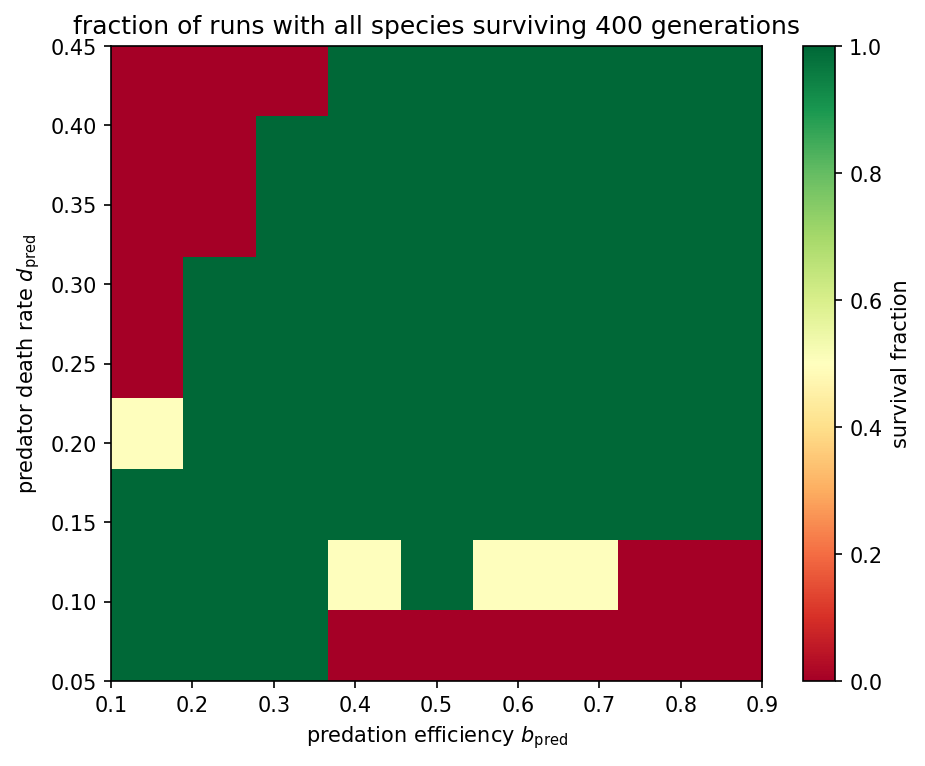
\includegraphics[width=0.75\textwidth]{ch5_survival_sweep}
\caption{Survival phase diagram: the fraction of runs (of a small
ensemble) in which all species persist for 400 generations, as the
predator's predation efficiency and death rate are varied.  Green marks
coexistence; red marks extinction.}
\label{fig:survival}
\end{figure}

One reason for the initial transients is that the initial spatial
arrangement of cell states is random, whereas the steady-state
distribution is far from random; the transient period involves the
spatial drift from the random initial configuration toward a more
optimal one (compare Figures~\ref{fig:eco-init}
and~\ref{fig:eco-2000}).  Another reason, visible in the phase
portrait, is that our initial state was a bit too lush with plant life,
placing the initial point off to one side of the main coil of the
trajectory.

\expand{This CA ecosystem is a spatial, individual-based analogue of
the Volterra--Lotka equations, and it illustrates a lesson that the
intervening decades have underscored: spatial structure changes
everything.  Where the mean-field differential equations predict either
neutral cycles or a single damped approach to equilibrium, spatially
extended predator/prey CA generate travelling waves, spiral patterns,
and persistent noisy oscillations sustained by local
desynchronization --- dynamics now central to theoretical ecology and
epidemiology.  The same mechanism drives spiral waves in the
Belousov--Zhabotinsky reaction and in models of cardiac fibrillation
mentioned in Chapter~1.  This ecosystem is also the springboard for
Chapter~\ref{ch:evolution}, which gives its creatures the ability to
\emph{move} and equips them with competing perceptual \emph{strategies},
turning the simulation into an evolutionary-game laboratory.}

The original edition tracked the same ecosystem out to 11{,}200
generations; the population curves continue their noisy, bounded
oscillation indefinitely, and the actual state continues to resemble
Figure~\ref{fig:eco-2000}.  The reader is
encouraged to reproduce such long runs --- now a matter of seconds
rather than an overnight computation --- and to rotate the phase
portrait interactively:

\begin{lstlisting}
from cadyn.ecosystem import Ecosystem
import numpy as np

eco = Ecosystem(n=200, p_prey=0.212, p_pred=0.029,
                rng=np.random.default_rng(11))
eco.run(11_200)
eco.plot_populations(sample_every=8)   # long-run population curves
ax = eco.plot_phase_portrait()         # rotate with ax.view_init(...)
\end{lstlisting}

\chapter{Qualitative Classification of CA}
\label{ch:classification}

The examples of the previous chapters exhibit a striking range of
long-term behavior.  Some settle quickly to a uniform or fixed state;
some fall into short cycles or simple periodic patterns; some, like the
mandalas of Chapter~4, produce intricate but ultimately self-similar
structure; and some, like the 1-dimensional Life of
Section~\ref{sec:life1d}, generate behavior that looks genuinely
unpredictable.  Stephen Wolfram proposed that this diversity, across
CA of every dimension, sorts into just four qualitative classes.

\section{Wolfram's Four Classes}

Starting a CA from a typical (often random) initial state and watching
its evolution, one observes one of four broad outcomes:

\begin{description}
\item[Class 1 --- homogeneous.] The system evolves to a single uniform
  state, independent of the initial condition.  All information about
  the starting configuration is lost; the basin-of-attraction field
  has a single point attractor.  (The 0-dimensional rule $f(x)=0$ of
  Section~\ref{sec:entropy} is the simplest example.)
\item[Class 2 --- periodic.] The system settles into stable or
  oscillating structures, possibly many of them, each localized.
  Changing a cell affects only a bounded region.  The additive rules
  producing Sierpi\'nski-like patterns are essentially of this class:
  simple, self-similar, and locally determined.
\item[Class 3 --- chaotic.] The system produces aperiodic,
  random-looking patterns.  A local change spreads at a finite speed to
  affect an ever-growing region --- sensitive dependence on initial
  conditions, the discrete analogue of chaos.  Many of the
  higher-modulus and non-additive rules of Chapters~3 and~4 fall
  here.
\item[Class 4 --- complex.] The system produces localized structures
  that move and interact in complicated ways, neither settling down
  (as in Class~2) nor dissolving into noise (as in Class~3).  This is
  the rarest and most interesting class.  Conway's Game of Life and the
  particle-like 1-dimensional Life of Section~\ref{sec:life1d} are the
  canonical examples.
\end{description}

The classes are qualitative and, in general, undecidable to determine
from the rule alone (see below); nonetheless they capture something
real.  Figure~\ref{fig:sixclasses} shows one elementary rule
(Section~\ref{sec:elementary}) from each class, evolved from the same
random initial row: Rule 160 empties the lattice (Class~1), Rule 108
freezes into stripes and blinkers (Class~2), Rule 30 boils into noise
(Class~3), and Rule 110 threads persistent structures through the chaos
(Class~4).

\begin{figure}[htbp]\centering
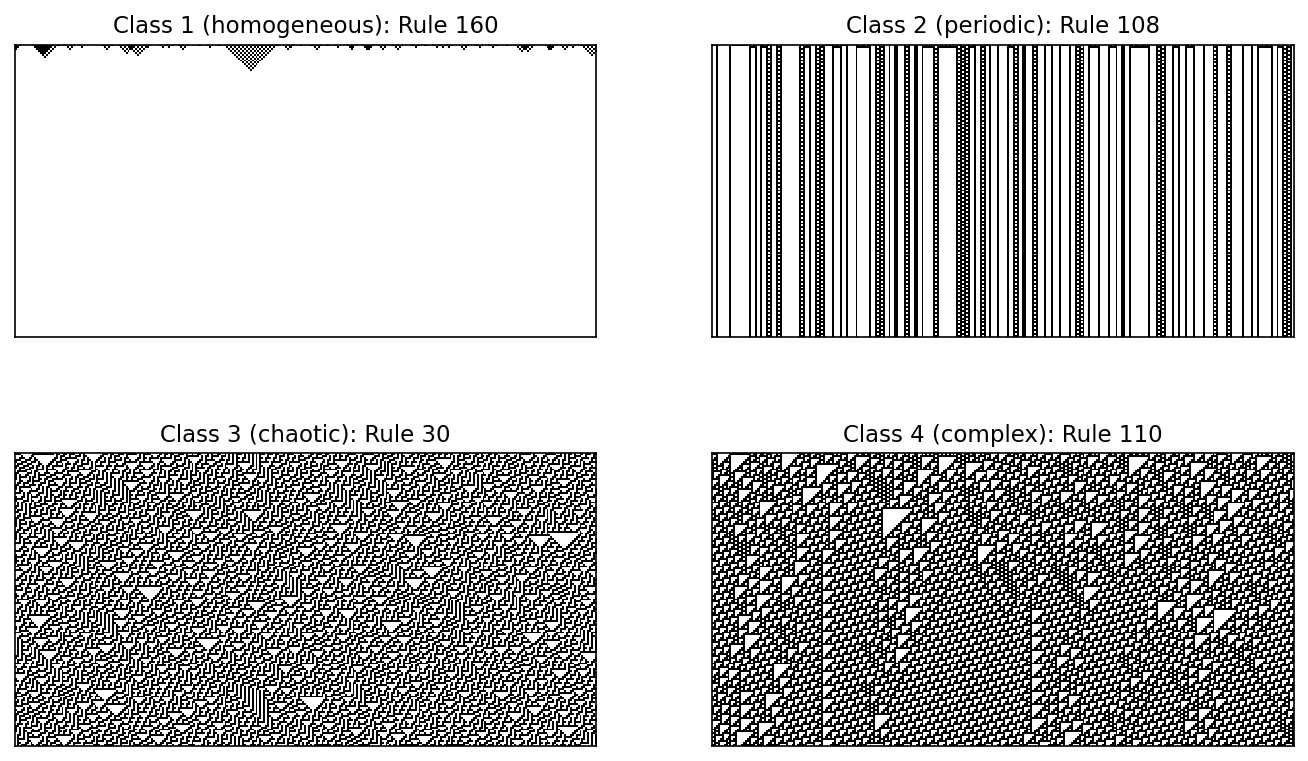
\includegraphics[width=\textwidth]{ch6_four_classes}
\caption{One elementary CA from each of Wolfram's four classes, all
started from the same random row.  Time runs downward.}
\label{fig:sixclasses}
\end{figure}

As one scans a parameter --- Wolfram's collaborator Christopher
Langton proposed the ``$\lambda$ parameter,'' roughly the fraction of
neighborhood configurations mapped to a nonzero state --- the typical
behavior passes from Class~1/2 order, through a narrow Class~4 regime,
into Class~3 chaos.  Langton dubbed this transitional regime the
\emph{edge of chaos} and conjectured that it is precisely there that a
CA can support the transmission, storage, and modification of
information required for computation.

\section{Computation at the Edge of Chaos}

The connection to computation is not merely metaphorical.  A Class~4 CA
has the three ingredients a computer needs: persistent structures that
\emph{store} information (still lifes, blinkers), moving structures that
\emph{transmit} it (gliders), and interactions that \emph{modify} it
(glider collisions implementing logic gates).  In Conway's Life these
ingredients suffice to build logic gates, wires, memory, and ultimately
a universal computer; Life is \emph{Turing complete}.  The same is true
of the 1-dimensional rule Wolfram numbered 110, proved universal by
Matthew Cook.

Figure~\ref{fig:rule110} shows Rule 110 evolving from a random initial
state.  Against a regular striped background, localized structures ---
the 1-dimensional analogues of Life's gliders --- travel at various
speeds, collide, and transform one another.  It is exactly this
repertoire of persistent, moving, interacting particles that Cook
marshalled into a proof of universality: suitably arranged particle
streams emulate a tag system, itself known to be Turing complete.

\begin{figure}[htbp]\centering
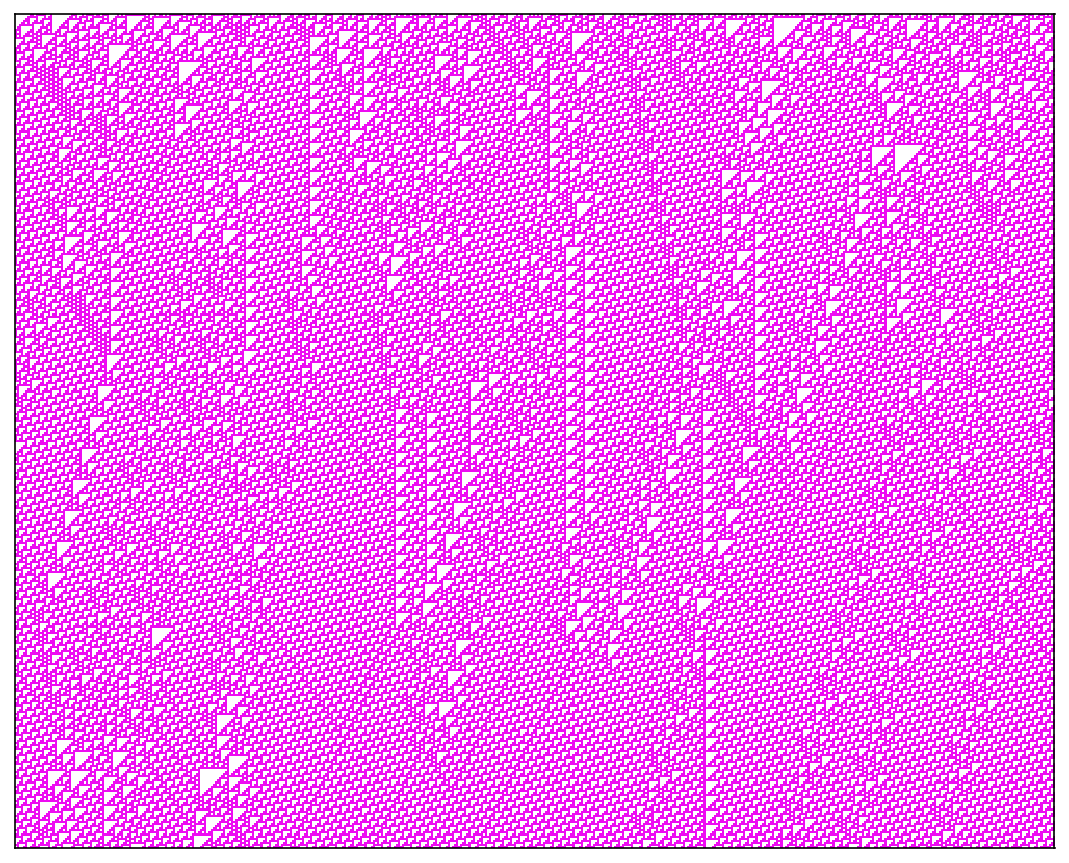
\includegraphics[width=0.9\textwidth]{ch6_rule110_detail}
\caption{Rule 110 from a random initial state (time downward):
particle-like structures drift across a periodic background and
interact when they meet --- the raw material of Cook's universality
proof.}
\label{fig:rule110}
\end{figure}

Universality has a sharp consequence: the long-term behavior of a
Class~4 CA is in general \emph{undecidable}.  There can be no algorithm
that, given an arbitrary initial state, decides whether a particular
cell ever becomes alive, whether the pattern dies out, or whether it
grows forever --- these are instances of the halting problem.  Wolfram
framed this as the \emph{principle of computational irreducibility}:
for such systems there is no shortcut, no closed-form solution, that
predicts the outcome faster than simply running the automaton
generation by generation.  This is in sharp contrast to the additive
CA of Sections~\ref{sec:poly1d} and~\ref{sec:poly2d}, whose polynomial
representation \emph{is} exactly such a shortcut.  The additivity that
made those systems tractable is the very property that keeps them out
of Class~4.

\section{Philosophical Reflections}

CA raise, in unusually concrete form, some old questions.

If a simple deterministic universe of cells can generate behavior that
is unpredictable in principle --- not merely in practice --- then
determinism and predictability come apart.  A Class~4 CA is fully
determined by its rule and initial state, yet no observer inside or
outside it can foresee its future without living through it.  This
offers a tidy resolution to a version of the free-will puzzle: a
system may be at once completely law-governed and computationally
irreducible, so that ``what it will do'' has no answer short of its
doing it.

The recurring phenomenon of this book --- simple local rules giving
rise to complex global order --- is precisely the phenomenon of
\emph{emergence} catalogued in Chapter~1: the origin of life,
morphogenesis, consciousness, cultural and economic dynamics.  CA do
not \emph{explain} these, but they furnish a proof of concept, an
existence theorem, that emergent complexity requires no complex or
mysterious cause.  A one-line rule is enough.

Finally, there is the tantalizing question of whether physics itself is
at bottom a cellular automaton --- whether space, time, and matter are
discrete and locally updated, with the smooth differential equations of
physics only their large-scale approximation, exactly as the
lattice-gas CA of Chapter~1 approximate fluid flow.

\expand{Wolfram pressed this program at book length in \emph{A New Kind
of Science} (2002), and the digital-physics hypothesis has since been
pursued (with varying reception) in his 2020 Wolfram Physics Project,
in work on quantum cellular automata, and in the ``it from bit'' and
holographic strands of theoretical physics.  Whether the universe
\emph{is} a cellular automaton remains open --- and may, fittingly, be
computationally irreducible.  Cook's proof that Rule~110 is universal
(conjectured by Wolfram in the 1980s) appeared in 2004; Langton's
edge-of-chaos hypothesis remains influential though contested.  What is
no longer in doubt is the book's central thesis: that cellular automata
are a serious mathematical laboratory for the study of how complexity
emerges from simplicity.}

\chapter{Evolutionary Dynamics: A Case Study}
\label{ch:evolution}

The ecosystem of Chapter~\ref{ch:ecosystem} was built to \emph{display}
predator/prey dynamics.  This chapter puts the same kind of machinery to
work \emph{answering a scientific question} --- and in doing so
introduces two ingredients the earlier model lacked: creatures that
\emph{move}, and creatures that carry competing \emph{strategies}
selected over evolutionary time.  The material is adapted from the
author's later study \emph{Veridical Perception and Evolutionary
Dynamics}; here we develop in full the compact mean-field model at its
core, whose every claim can be checked in a few lines of Python, and
describe the spatial simulation in prose, since it is a direct
descendant of \texttt{cadyn.ecosystem}.

\section{The Question: Does Evolution Favor Accurate Perception?}

It is tempting --- and widely assumed among cognitive scientists and AI
researchers --- that natural selection favors \emph{veridical}
perception, perception that reports the world as it actually is.
Accurately registering reality surely helps one survive.  Donald Hoffman
and colleagues challenged this in a 2010 paper, \emph{Natural Selection
and Veridical Perceptions}, arguing that selection optimizes
\emph{fitness}, not truth, and that the two can come apart: a cheap,
fast, systematically \emph{inaccurate} perceptual strategy can outcompete
an accurate but costly one.

The intuition is a matter of timing.  Accurate perception takes
processing --- more neural layers, more computation, more time --- and
neural signals are slow.  In a life-or-death moment, a bird that takes
an extra beat to resolve exactly what it is seeing may already be in the
cat's jaws.  The question is whether this cost is enough to select
\emph{against} veridical perception, and if so, when.

\expand{Hoffman has since developed this line into the \emph{Interface
Theory of Perception}: the thesis that our perceptions are like a
desktop interface --- useful, fitness-tuned icons that hide rather than
reveal the underlying reality, much as a file icon tells you nothing
about voltages on a disk.  His 2019 book \emph{The Case Against Reality}
presents the ``Fitness-Beats-Truth'' theorem, which within a class of
evolutionary-game models shows truth-tuned strategies are driven to
extinction by fitness-tuned ones of equal complexity with probability
approaching one as the world's complexity grows.  The CA experiments of
this chapter are a small, concrete, spatially explicit instance of the
same phenomenon.}

\section{A Mean-Field Model of Strategy Competition}
\label{sec:meanfield}

Consider one species with several competing perceptual strategies.
Strategy~$i$ has a fixed \emph{probability of success} $p_i$ ---
loosely, the chance it survives the encounters of one generation --- and
we take this $p_i$ to be its fitness.  For the running example we use
three strategies with
\[
  p = (p_R,\, p_P,\, p_V) = (0.6,\ 0.75,\ 0.9),
\]
standing for a \textbf{R}andom (non-perceiving), a \textbf{P}robabilistic
(sometimes-perceiving), and a \textbf{V}eridical (always-perceiving)
strategy.  Under the natural reading in which more accurate perception
yields more successful encounters, $V$ has the highest bare fitness.

Now place the strategies on the 2-dimensional toroidal lattice of the
previous chapters, one strategy per cell, with the eight-cell Moore
neighborhood.  The update is deliberately simple and partly stochastic:
at each tick a cell keeps its own strategy with probability equal to its
success rate, and otherwise switches to the majority strategy among its
neighbors.  A high-fitness strategy is ``sticky'' --- its holders rarely
defect --- while low-fitness cells readily convert to whatever surrounds
them.

To analyze this, make one very reasonable mean-field assumption: that the
probability a given neighbor is of type~$i$ equals that type's current
population proportion $s_i$.  Writing $s(t) = (s_1, s_2, s_3)^{\mathsf T}$
for the proportion vector, the dynamics become a matrix iteration
\begin{equation}
  s(t+1) = W(t)\, s(t),
  \label{eq:meanfield}
\end{equation}
where the transition matrix is itself a function of the current state:
\begin{equation}
  W(t) =
  \begin{bmatrix}
    p_1 + (1-p_1)s_1 & (1-p_2)s_1 & (1-p_3)s_1\\
    (1-p_1)s_2 & p_2 + (1-p_2)s_2 & (1-p_3)s_2\\
    (1-p_1)s_3 & (1-p_2)s_3 & p_3 + (1-p_3)s_3
  \end{bmatrix}.
\end{equation}
Each column $j$ sums to 1: a cell of type $j$ either keeps its type
(diagonal term $p_j$) or, with probability $1-p_j$, converts to
type~$i$ with probability $s_i$.  This is like a Markov chain, except
that the transition matrix drifts with the population it governs.

Iterating \eqref{eq:meanfield} from any interior start drives the system
to a vertex of the simplex: the fittest strategy takes over completely
and the rest go extinct.  Figure~\ref{fig:mf-runs} shows this for the
equal start $(\tfrac13,\tfrac13,\tfrac13)$ and the uneven start
$(0.5, 0.3, 0.2)$; in both, $V$ wins.  Notably, $V$ wins the second race
\emph{even though it starts as the smallest population} --- higher
fitness, not a head start, decides the outcome.

\begin{figure}[htbp]\centering
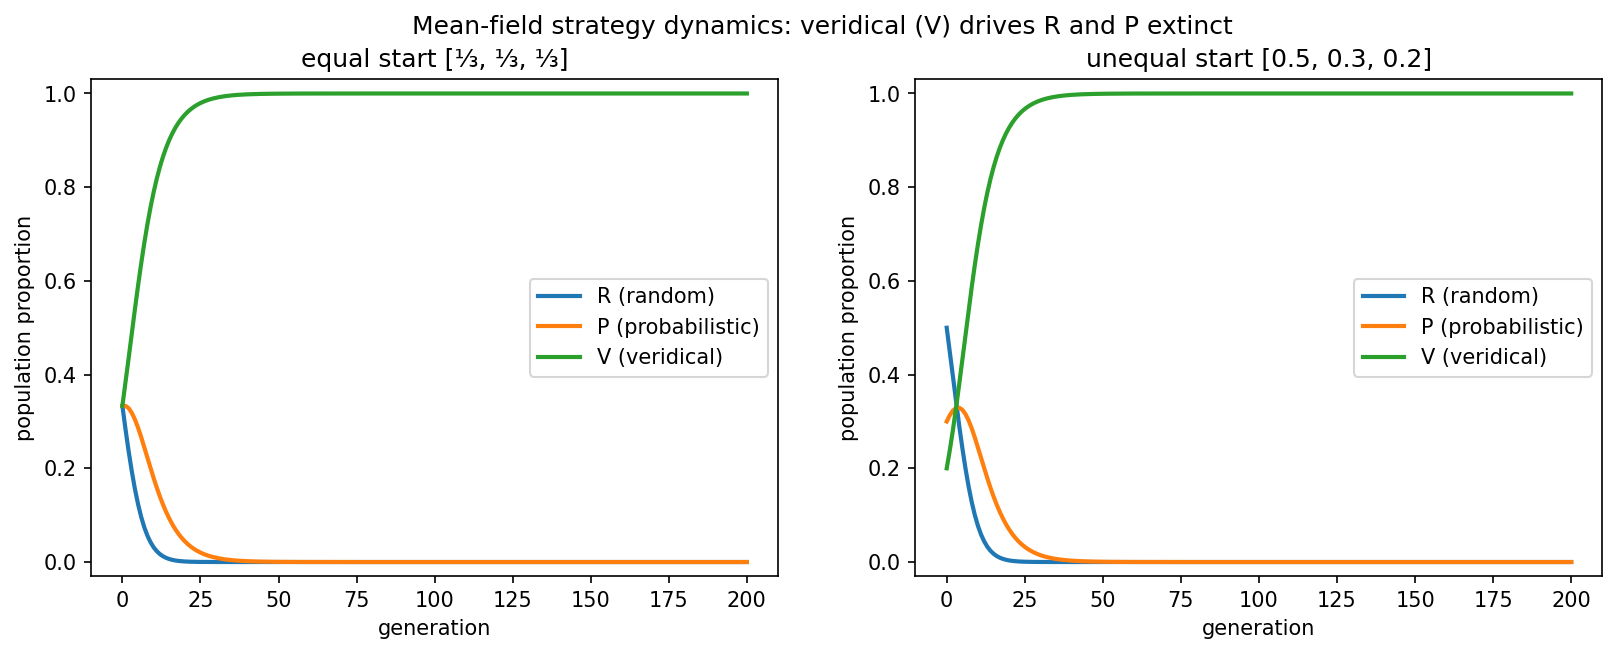
\includegraphics[width=\textwidth]{ch7_meanfield_runs}
\caption{The mean-field strategy dynamics from two initial conditions.
The veridical strategy $V$ ($p=0.9$) drives the random and
probabilistic strategies to extinction, even when (right) it begins as
the least common.}
\label{fig:mf-runs}
\end{figure}

The three-strategy state lives on the 2-simplex --- a triangle whose
corners are the pure strategies and whose interior is every mixture.
Figure~\ref{fig:mf-simplex} plots trajectories from many random starts;
every one flows to the $V$ corner.

\begin{figure}[htbp]\centering
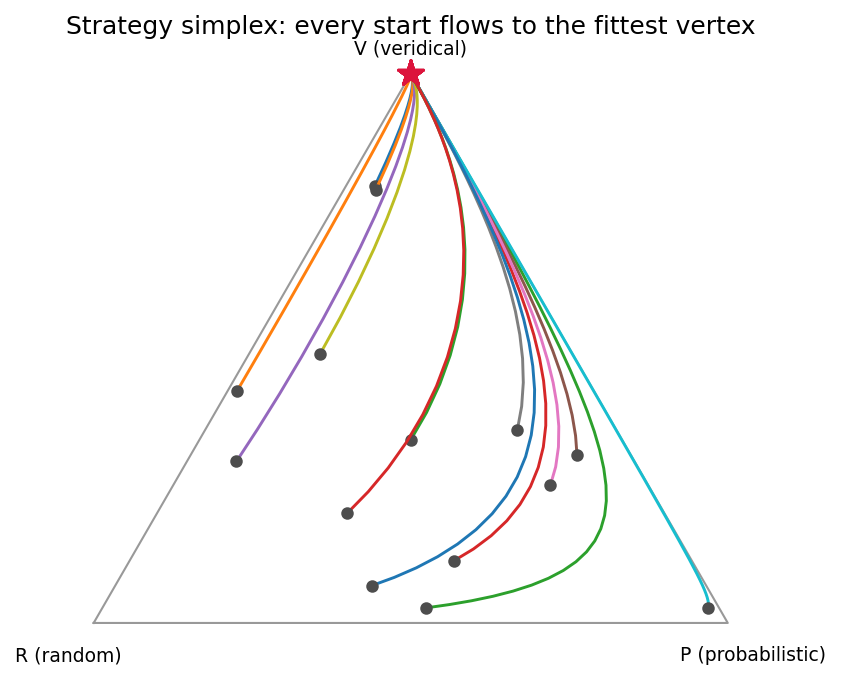
\includegraphics[width=0.7\textwidth]{ch7_simplex}
\caption{Trajectories of the proportion vector on the strategy simplex.
Circles mark starts, stars mark the shared destination: the
veridical vertex.}
\label{fig:mf-simplex}
\end{figure}

\subsection*{A Lemma, and a coordinate-free form}

The matrix $W(t)$ is unwieldy, but the map it defines has a clean
closed form.  Let ``$\circ$'' denote the elementwise (Hadamard) product,
$\vec 1$ the all-ones vector, and $I$ the identity.

\begin{lemma}
The update $s(t+1) = W(t)\,s(t)$ can be written, in any dimension, as
\begin{equation}
  s(t+1) = \Bigl(\, p \circ I \;+\; \vec 1\,\bigl((\vec 1 - p)\circ s\bigr)^{\mathsf T}\Bigr)\circ s,
  \label{eq:lemma}
\end{equation}
equivalently and more concretely as
\begin{equation}
  s(t+1) \;=\; p \circ s \;+\; s\,\bigl\langle \vec 1 - p,\ s\bigr\rangle,
  \label{eq:lemma-scalar}
\end{equation}
where $\langle\,\cdot\,,\cdot\,\rangle$ is the ordinary dot product.
\end{lemma}

\begin{proof}
Suppressing the $t$-dependence and writing $q_j = 1-p_j$, the
$i$\textsuperscript{th} component of $W s$ is
\[
  (Ws)_i = \Bigl(p_i + q_i s_i\Bigr)s_i
           + \sum_{j\neq i} q_j s_i s_j
         = p_i s_i + s_i \sum_{j} q_j s_j
         = p_i s_i + s_i\,\langle \vec 1 - p,\ s\rangle,
\]
which is exactly \eqref{eq:lemma-scalar}; expression \eqref{eq:lemma}
is the same computation arranged as a Hadamard product of the bracketed
matrix (diagonal $p_i$, every row equal to $((\vec 1 - p)\circ s)^{\mathsf T}$)
with the column $s$, followed by the row sum.  Nothing in the derivation
used $n=3$, so the form is valid in every dimension.
\end{proof}

The scalar form \eqref{eq:lemma-scalar} is illuminating: each generation
scales strategy~$i$ by its own fitness $p_i$ and then adds back a share
$s_i$ of the total ``defection mass'' $\langle \vec1 - p, s\rangle$.
Because the surviving-and-switching bookkeeping is exact, the true map
conserves $\sum_i s_i$; in floating-point iteration one renormalizes each
step, which is what ``population \emph{proportions}'' means anyway.  The
module \texttt{cadyn.evolution} provides all three formulations and a
routine \texttt{verify\_lemma} confirming they agree --- for the worked
example and for hundreds of random cases in dimensions 2 through 8.

\subsection*{An empirical theorem}

Simulation makes the following extremely plausible; a formal proof
eluded the original study and we state it as the paper did.

\begin{theorem}[empirical]
Let $s(0)$ be any interior point of the probability simplex
($s_i(0) > 0$ for all $i$), and suppose the fitness vector has a unique
maximum, $p_k > p_j$ for all $j \neq k$.  Then $s(t) \to e_k$ as
$t\to\infty$, where $e_k$ is the standard basis vector with a $1$ in
position $k$.
\end{theorem}

The routine \texttt{cadyn.evolution.dominant\_strategy\_wins} tests one
initial condition; across 500 random starts in three dimensions, and 100
each in dimensions 4, 6, and 10, the unique fittest strategy won every
time --- somewhat stronger evidence than the original paper marshalled.
A natural next step, which the original study flagged as future work, is
to find a replicator system approximating this map and prove convergence
analytically; the replicator equation is the standard bridge from such
population updates to a dynamical system with known convergence theory.

The mean-field model can also \emph{preview} the chapter's central
reversal.  Nothing in it explains why $V$ should be fittest --- that is
an input.  If accurate perception carries a computational cost, we can
model that cost crudely by lowering $V$'s effective success rate.
Figure~\ref{fig:mf-penalty} repeats the equal-start race with $V$'s
fitness cut from $0.9$ to $0.55$, below $P$'s $0.75$: now the
probabilistic strategy sweeps the board and veridical perception is the
one driven extinct.  The mean-field model thus contains both outcomes;
which one obtains depends entirely on whether accurate perception is
worth its price.  The spatial model of the next section supplies that
price from first principles, as a cost in \emph{time}.

\begin{figure}[htbp]\centering
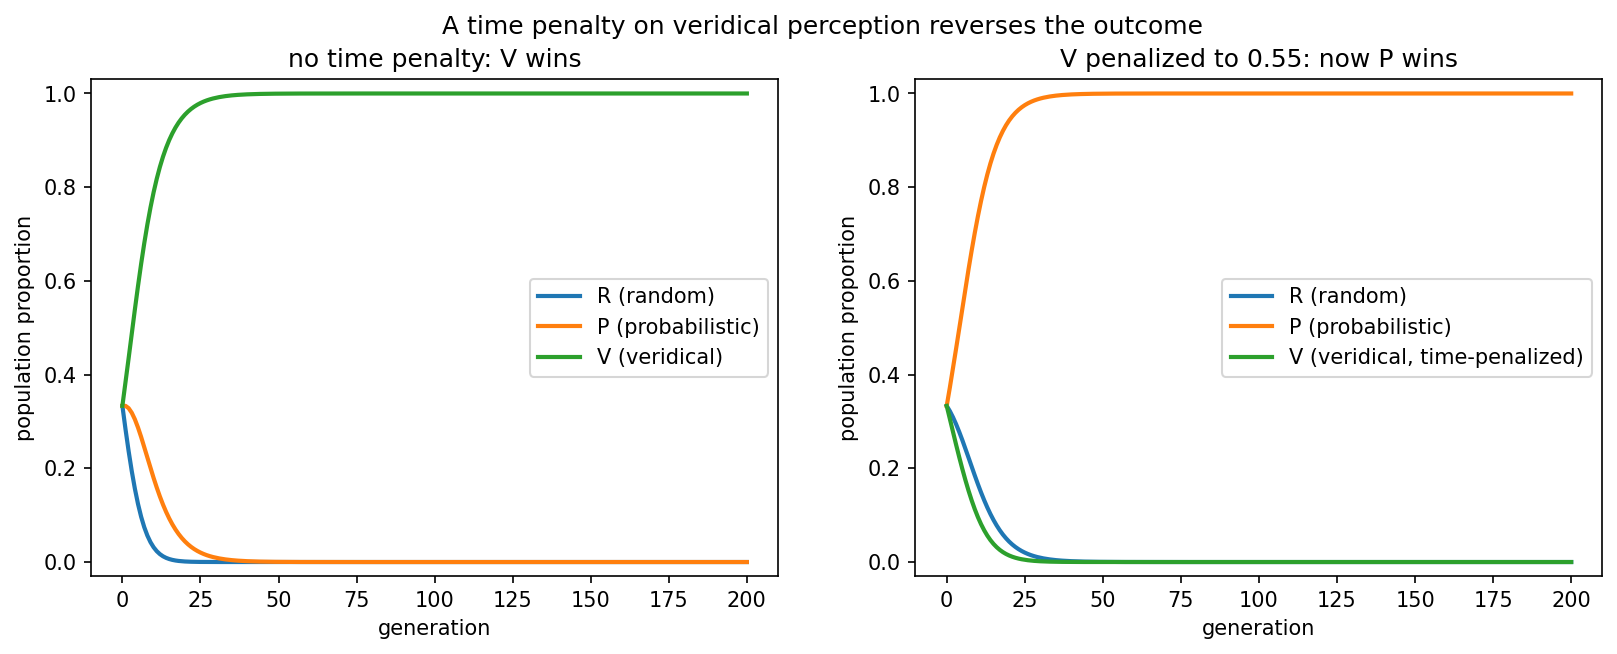
\includegraphics[width=\textwidth]{ch7_penalty}
\caption{Left: with no cost, the veridical strategy wins (as before).
Right: charging veridical perception a computational cost --- modeled
here by lowering its effective fitness below the probabilistic
strategy's --- reverses the outcome, and $V$ goes extinct.}
\label{fig:mf-penalty}
\end{figure}

\section{The Spatial Experiment: Movement, Fitness, and a Time Penalty}
\label{sec:spatial-evolution}

The mean-field model already vindicates Hoffman's logic, but only as
abstractly as his own argument: it \emph{assumes} $V$ has the highest
fitness and then shows the fittest wins.  It says nothing about
\emph{why} veridical perception might fail to be fittest.  For that we
need a model where perception actually costs something, and the natural
vehicle is a spatial ecosystem in the manner of
Chapter~\ref{ch:ecosystem} --- extended, crucially, with
\emph{movement}.

\subsection*{What is added to the Chapter~5 ecosystem}

The second experiment keeps the toroidal lattice, the plant/prey/predator
roles, the stochastic asynchronous updates, and the population and
phase-portrait diagnostics of Chapter~\ref{ch:ecosystem}, and layers on:

\begin{itemize}
\item \textbf{Movement.} Creatures (birds and cats) take random walks: a
  creature moves by copying its state into a vacant neighboring cell and
  vacating its own.  Eating is movement --- a bird eats a plant by
  stepping onto it; a cat eats a bird by pouncing onto its cell.  (The
  author notes that mobile creatures in an evolutionary-game CA appear
  to be novel, tracing the idea to his own 1997 work --- the very book
  this volume revises.)
\item \textbf{Individual fitness, birth, and death.} Each creature
  carries a fitness counter: eating raises it, each idle tick lowers it,
  zero means starvation, and crossing a threshold triggers haploid
  reproduction onto a neighboring empty or plant cell.  Unlike the
  Chapter~5 model, which tracked only population \emph{counts}, here
  fitness is an attribute of each individual.
\item \textbf{Perceptual strategies.} Every bird and every cat carries
  one of three strategies --- $R$ (random walk, no perception), $V$
  (veridical: birds flee perceived cats, cats pounce on perceived
  birds), and $P$ (do $V$ with probability $\rho$, else $R$).  This is
  the mean-field model's $R/P/V$ competition, now embodied in moving,
  eating, breeding animals.
\end{itemize}

Including plants alongside prey and predators yields a
rock-paper-scissors (``Rochambeau'') structure, expressed --- as the
author wryly notes --- through negations: no plants starves the birds,
no birds starves the cats, and no cats lets the birds strip the plants.
That cyclic non-transitivity may be exactly what underlies the dynamic
stability of a broad range of Lotka--Volterra systems; flattening it by
omitting plants obscures the mechanism.

\subsection*{The result, and the reversal}

Run without any timing asymmetry, the spatial model echoes the
mean-field one: the veridical strategies drive the others to extinction,
first the random strategies and then the probabilistic ones, for both
birds and cats.  The surviving bird/cat subsystem settles into the noisy,
damped Lotka--Volterra oscillation familiar from
Chapter~\ref{ch:ecosystem}, spiralling toward an interior Nash
equilibrium; in the reported run the normalized bird/cat proportions
converge near $[0.738,\, 0.262]$ with strikingly small steady-state
variance, and an FFT of the population series reveals a dominant cycle of
about 18 generations.  So far, ``veridical perception wins again.''

The decisive experiment introduces the cost of perception as a cost in
\emph{time}.  In the baseline simulation, cats happen to move first ---
they perceive and act before birds do.  To penalize veridical
perceivers for the processing their accuracy requires, the veridical
creatures are made to move \emph{last}: they pay for their better
picture of the world with a beat of delay, exactly the slow-neuron cost
of the opening question.  Under this single change the balance shifts.
The probabilistic strategy, now no longer strictly dominated, competes
with the veridical one on even terms and is no longer driven to
extinction; a slow-but-accurate strategy can be beaten by a
faster, less accurate one.  A pair of thought experiments makes the
mechanism vivid: a bird that resolves ``cat'' a moment too late is
already caught, and a cat that resolves ``bird'' too late goes hungry
--- and repeated, either lag is lethal to the strategy that carries it.

\expand{This is the CA analogue of Hoffman's claim and, more broadly, a
lesson machine learning has relearned: depth is not free.  Because
neural signals are slow, biological brains run \emph{shallow} networks
compared with the very deep ones routinely trained today; a perceptual
system optimized purely for accuracy, with no regard to latency, is not
the system evolution builds.  ``To have survival value, perceptions must
be fast'' --- a constraint now visible in real-time robotics and
edge-inference, where a slightly-worse-but-faster model routinely beats a
slightly-better-but-slower one.}

\section{An Emergent Curiosity: Fitness Collapse Before Extinction}

One observation from the spatial runs deserves flagging because it was
not sought and is not obviously an artifact.  Tracking the \emph{mean
fitness} of each sub-population over time, the author found that a
strategy's mean fitness tends to \emph{oscillate wildly in the moments
before that strategy goes extinct}, and that the overall mean fitness of
the whole ecosystem \emph{steps down} with each extinction event.  Both
effects invite the question the original study left open: are they
quirks of this particular CA, or do they echo something real ---
critical-slowing-down and variance-inflation of the kind studied as
\emph{early-warning signals} of tipping points in real ecosystems?  The
CA is cheap enough to make this a natural thing to probe systematically,
and the tools of Chapter~\ref{ch:ecosystem} (population and phase-space
diagnostics) apply directly.

\section{Reflection}

Two models, one abstract and one spatially explicit, independently
support Hoffman's conclusion: veridical perception is favored by
selection \emph{until} its computational cost is reckoned, after which a
faster, less accurate strategy can win.  The mean-field model is fully
reproduced and checked in \texttt{cadyn.evolution}; the spatial model,
being a direct extension of \texttt{cadyn.ecosystem} with movement and
per-individual strategies, is left as a described experiment and an
invitation.  It closes a loop with Chapter~\ref{ch:ecosystem}: the
predator/prey CA that began as a way to \emph{watch} population dynamics
turns out, with movement and strategies added, to be a laboratory for one
of the sharper questions in the science of the mind --- whether the world
we perceive is the world as it is, or merely the world as it pays to see.


\appendix
\chapter{Modular Arithmetic}
\label{app:modular}

Modular arithmetic (sometimes ``clock arithmetic'') is ordinary
integer arithmetic --- addition and multiplication --- with one extra
step: after each operation, divide by the modulus and report only the
remainder.  For example, with modulus 5,
\[
  3 + 4 = 7 \equiv 2 \pmod 5,
\]
read ``three plus four is congruent to two modulo 5,'' since 5 goes
into 7 once with remainder 2.  Any integer reduces modulo 5 to one of
$0,1,2,3,4$: if positive, take the remainder on division by 5; if
negative, add 5 repeatedly until the result lies in that range.  Since
$5 \equiv 0 \pmod 5$, adding 5 never changes a result mod 5.  The
additive inverse of 1 is $-1$, and $-1+5 = 4$, so $-1 \equiv 4
\pmod5$.  In general
\[
  n \equiv 0 \pmod n, \qquad -1 \equiv n-1 \pmod n .
\]

Modulo-2 arithmetic has only two digits, $0$ and $1$, and reduces to
three rules (writing $=$ for congruence mod 2):
\[
  0 + 0 = 0, \qquad 0 + 1 = 1, \qquad 1 + 1 = 0 .
\]
These are exactly the rules of the ``exclusive or'' operation of
Boolean algebra, of central importance in the design of digital
circuits.  In Python, the operator is spelled \texttt{\%}
(\texttt{7 \% 5} evaluates to \texttt{2}), and it is applied
element-wise by NumPy: \texttt{np.mod(array, k)}.

\chapter{Pascal's Triangle}
\label{app:pascal}

The simplest construction of Pascal's triangle: start with a single 1;
each subsequent row is obtained by adding adjacent entries of the row
above (treating missing entries as 0):
\[
\begin{array}{ccccccccc}
 & & & & 1\\
 & & & 1 & & 1\\
 & & 1 & & 2 & & 1\\
 & 1 & & 3 & & 3 & & 1\\
1 & & 4 & & 6 & & 4 & & 1
\end{array}
\]
The entries are the \emph{binomial coefficients}, arising in the
expansion
\[
  (a+b)^n = \sum_{k=0}^{n} \binom{n}{k} a^k b^{n-k},
  \qquad \binom{n}{k} = \frac{n!}{k!\,(n-k)!},
\]
where $\binom{n}{k}$ sits at position $k$ of row $n$ (numbering rows
and positions from zero).

Reduced modulo 2, Pascal's triangle becomes an intricate pattern of
ones and zeros --- recognizable as none other than Sierpi\'nski's
gasket (Figure~\ref{fig:pascal2}).  This is exactly the pattern
produced by the additive CA with kernel $[1\;0\;1]$ modulo 2
(Section~\ref{sec:kernel101}), as the polynomial analysis of
Section~\ref{sec:poly1d} makes precise: the coefficients
$\binom{t}{i}$ appear directly in the closed form for that rule.
Computing $2^n$ rows of Pascal's triangle mod 2 yields a figure
resembling the approximation $S_n$ to the gasket
(Appendix~\ref{app:sierpinski}).

\begin{figure}[htbp]\centering
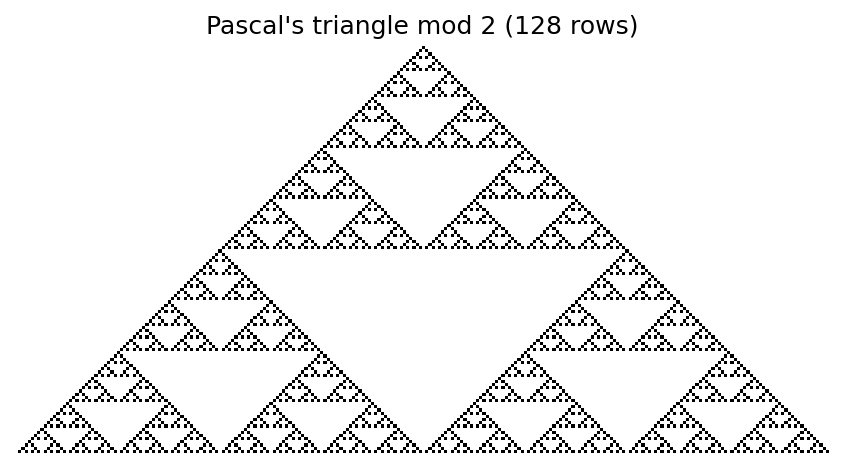
\includegraphics[width=0.7\textwidth]{appB_pascal_mod2}
\caption{Pascal's triangle modulo 2, 128 rows --- successive
approximations to Sierpi\'nski's gasket.}
\label{fig:pascal2}
\end{figure}

\chapter{Geometric Construction of Sierpi\'nski's Gasket}
\label{app:sierpinski}

In 1915 Wac\l{}aw Sierpi\'nski described the following geometric
construction of the fractal triangle now bearing his name.  Begin with
a filled equilateral triangle $S_0$.  To construct $S_1$, remove the
inverted middle triangle whose sides have half the length of the
original's.  To construct $S_2$, apply the same operation to each of
the three triangles composing $S_1$; to construct $S_3$, apply it to
each of the nine triangles composing $S_2$; and so on
(Figure~\ref{fig:sierp-construct}).

\begin{figure}[htbp]\centering
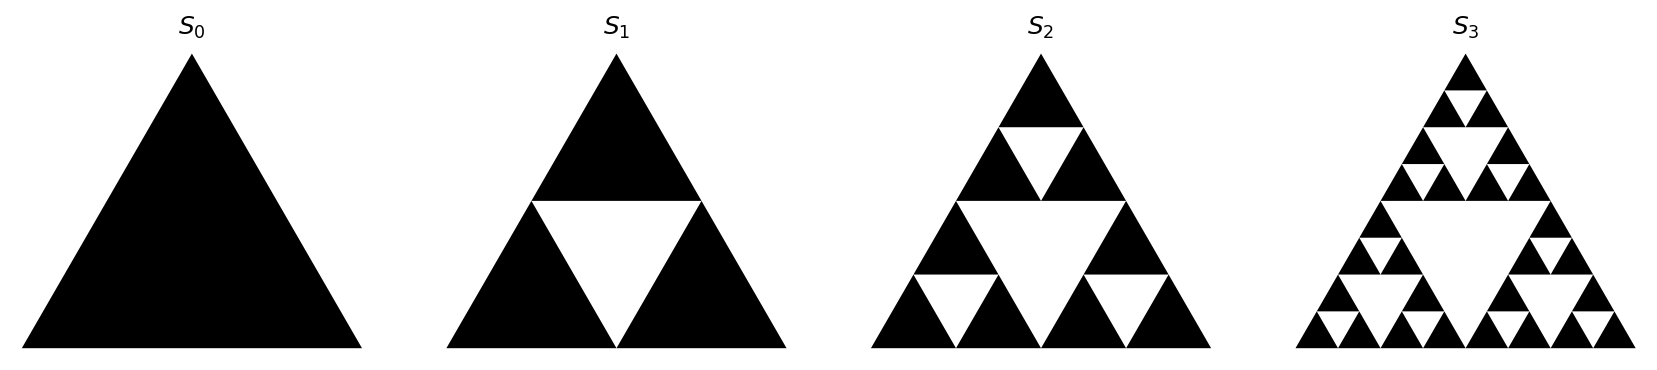
\includegraphics[width=\textwidth]{appC_sierpinski_construction}
\caption{The first four approximations $S_0, S_1, S_2, S_3$ to
Sierpi\'nski's gasket.}
\label{fig:sierp-construct}
\end{figure}

Continuing indefinitely yields a sequence $S_0, S_1, S_2, \dots$ of
better and better approximations; the gasket itself is the limit.  It
has zero area and Hausdorff dimension $\log 3 / \log 2 \approx 1.585$.
The CA with rule $[1\;0\;1]$ modulo 2, evolved for $2^{\,n+1}$
generations, produces a figure resembling $S_n$; the 256-generation run
of Figure~\ref{fig:sierp2} looks like $S_7$.  That three quite
different constructions --- a geometric removal process, Pascal's
triangle mod 2, and an additive CA --- converge on the same figure is a
small marvel worth pausing over.

\chapter{The Euler Totient Function}
\label{app:totient}

Euler's totient function $\varphi$ features prominently in number
theory.  For a positive integer $n$,
\[
  \varphi(n) = \text{the count of integers in } \{1,\dots,n\}
  \text{ that are relatively prime to } n,
\]
where two integers are \emph{relatively prime} if their only common
positive divisor is 1.  Thus 6 and 10 are not relatively prime (both
divisible by 2), while 9 and 10 are.  By convention $\varphi(1)=1$.
For a prime $p$ every smaller positive integer is coprime to it, so
\[
  \varphi(p) = p - 1 ,
\]
placing $\varphi$'s local maxima at the primes and its local minima at
integers with many factors (Figure~\ref{fig:totient-plot}).  More
generally, $\varphi$ is multiplicative and
$\varphi(p^a) = p^a - p^{a-1}$, giving the product formula
$\varphi(n) = n\prod_{p \mid n}(1 - 1/p)$.

\begin{figure}[htbp]\centering
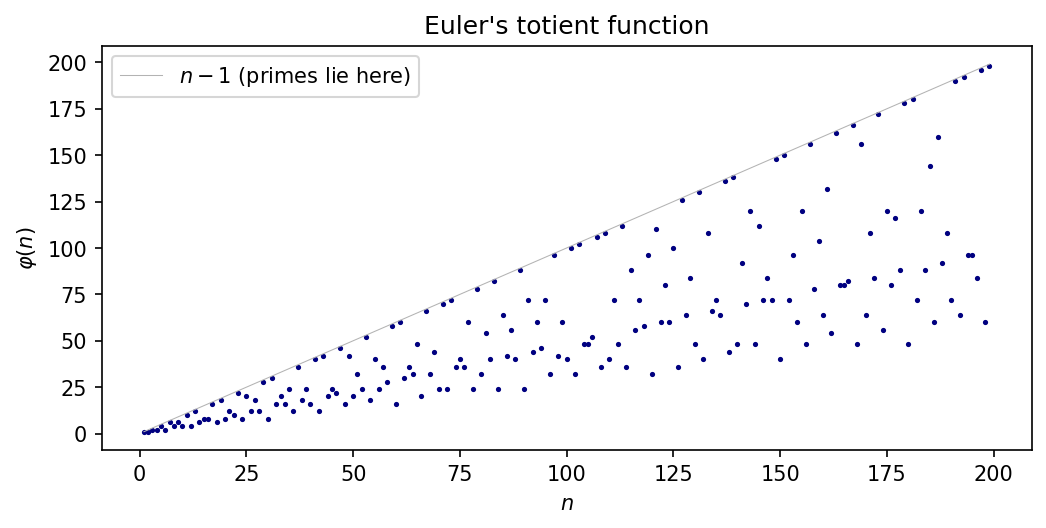
\includegraphics[width=0.85\textwidth]{appD_totient}
\caption{Euler's totient function for $n < 200$.  Primes lie on the
upper line $\varphi(n)=n-1$.}
\label{fig:totient-plot}
\end{figure}

A short table:

\begin{center}
\begin{tabular}{r|l|r}
\toprule
$n$ & integers coprime to $n$ & $\varphi(n)$\\
\midrule
 2 & 1                         & 1\\
 3 & 1, 2                      & 2\\
 4 & 1, 3                      & 2\\
 5 & 1, 2, 3, 4                & 4\\
 6 & 1, 5                      & 2\\
 7 & 1, 2, 3, 4, 5, 6          & 6\\
 8 & 1, 3, 5, 7                & 4\\
 9 & 1, 2, 4, 5, 7, 8          & 6\\
10 & 1, 3, 7, 9                & 4\\
12 & 1, 5, 7, 11               & 4\\
\bottomrule
\end{tabular}
\end{center}

The module \texttt{cadyn.numtheory} computes $\varphi$ both singly
(\texttt{totient(n)}) and as a sieve over a range
(\texttt{totient\_table(limit)}); the latter is used by the
Euler-totient CA rule of Section~\ref{sec:totient}, with the convention
$\varphi(0)=0$ so that a dead (zero) cell contributes nothing to its
neighbors' sums.


\backmatter
\chapter*{Bibliography}
\addcontentsline{toc}{chapter}{Bibliography}

\begin{thebibliography}{99}

\bibitem{gardner1970} Gardner, M. (1970).
  ``The fantastic combinations of John Conway's new solitaire game
  `life'.'' \emph{Scientific American} \textbf{223}(4), 120--123.

\bibitem{vonneumann1966} von Neumann, J. (1966).
  \emph{Theory of Self-Reproducing Automata} (edited and completed by
  A.~W.~Burks). University of Illinois Press.

\bibitem{shannon1948} Shannon, C.~E. (1948).
  ``A mathematical theory of communication.''
  \emph{Bell System Technical Journal} \textbf{27}, 379--423 and
  623--656.

\bibitem{wolfram1984} Wolfram, S. (1984).
  ``Universality and complexity in cellular automata.''
  \emph{Physica D} \textbf{10}, 1--35.

\bibitem{wolfram2002} Wolfram, S. (2002).
  \emph{A New Kind of Science}. Wolfram Media.

\bibitem{wuensche1992} Wuensche, A. and Lesser, M. (1992).
  \emph{The Global Dynamics of Cellular Automata: An Atlas of Basin of
  Attraction Fields of One-Dimensional Cellular Automata}.
  Addison-Wesley. (The atlas referred to in Section~\ref{sec:k5n21}.)

\bibitem{toffoli1987} Toffoli, T. and Margolus, N. (1987).
  \emph{Cellular Automata Machines: A New Environment for Modeling}.
  MIT Press.

\bibitem{langton1990} Langton, C.~G. (1990).
  ``Computation at the edge of chaos: phase transitions and emergent
  computation.'' \emph{Physica D} \textbf{42}, 12--37.

\bibitem{cook2004} Cook, M. (2004).
  ``Universality in elementary cellular automata.''
  \emph{Complex Systems} \textbf{15}, 1--40. (Proves Rule 110
  universal.)

\bibitem{berlekamp1982} Berlekamp, E.~R., Conway, J.~H., and Guy,
  R.~K. (1982). \emph{Winning Ways for Your Mathematical Plays},
  Vol.~2. Academic Press. (Universality of Life.)

\bibitem{lagarias2010} Lagarias, J.~C., ed. (2010).
  \emph{The Ultimate Challenge: The $3x+1$ Problem}.
  American Mathematical Society.

\bibitem{tao2019} Tao, T. (2022).
  ``Almost all orbits of the Collatz map attain almost bounded
  values.'' \emph{Forum of Mathematics, Pi} \textbf{10}, e12.
  (First circulated 2019.)

\bibitem{barina2020} Barina, D. (2021).
  ``Convergence verification of the Collatz problem.''
  \emph{The Journal of Supercomputing} \textbf{77}, 2681--2688.

\bibitem{sierpinski1915} Sierpi\'nski, W. (1915).
  ``Sur une courbe dont tout point est un point de ramification.''
  \emph{Comptes Rendus} \textbf{160}, 302--305.

\bibitem{harris2020} Harris, C.~R.\ et al. (2020).
  ``Array programming with NumPy.''
  \emph{Nature} \textbf{585}, 357--362.

\bibitem{virtanen2020} Virtanen, P.\ et al. (2020).
  ``SciPy 1.0: fundamental algorithms for scientific computing in
  Python.'' \emph{Nature Methods} \textbf{17}, 261--272.

\bibitem{hoffman2010} Hoffman, D.~D., Singh, M., and Mark, J. (2010).
  ``Natural selection and veridical perceptions.''
  \emph{Journal of Theoretical Biology} \textbf{266}(4), 529--539.

\bibitem{hoffman2019} Hoffman, D.~D. (2019).
  \emph{The Case Against Reality: Why Evolution Hid the Truth from Our
  Eyes}. W.~W.~Norton.

\bibitem{friedman2016} Friedman, D. and Sinervo, B. (2016).
  \emph{Evolutionary Games in Natural, Social, and Virtual Worlds}.
  Oxford University Press.

\bibitem{kahneman2011} Kahneman, D. (2011).
  \emph{Thinking, Fast and Slow}. Farrar, Straus and Giroux.

\bibitem{espericueta2020} Espericueta, R. (2020).
  ``Veridical Perception and Evolutionary Dynamics.'' Course study,
  Applied Machine Learning Lab, UC Santa Cruz.

\end{thebibliography}

\vspace{2em}
\noindent\textbf{Related links.}\quad
The complete Python source (\texttt{cadyn} package), the figure-
and appendix-generation scripts, and the LaTeX source of this book are
distributed together.  See the \texttt{README} for installation and a
guided tour.

\end{document}
